% !TEX encoding = UTF-8 Unicode
% !BIB TS-program = biber 
% !BIB program = biber    

% This file is MIT-Thesis.tex, a LaTeX template for formatting an MIT thesis with the mitthesis class.
%
% Version: 1.11, 2023/11/02
%
% Author: John H. Lienhard, copyright 2023. Reuse under the MIT license: https://ctan.org/license/mit 

% Documentation is here: https://ctan.org/pkg/mitthesis

%% Don't modify the \DocumentMetadata command unless you know what it does. 
%% If this command throws an "undefined" error, your latex system is out of date: try commenting this command out.
\DocumentMetadata{ 
	pdfstandard = a-2b,
	pdfversion  = 1.7,
	lang		= en-US,
%	debug		= {xmp-export}, % uncomment to output a separate xmpi file showing the metadata
}
%%%%%%%%%%%%%%%%%%%%%%%%%%%%%%%%%%%%%%%

\documentclass[twoside]{mitthesis} %,fontset=libertine, fontset=newtx-sans-text, fontset=heros-stix2, fontset=stix2
%
% option [twoside]		gives facing-page behavior for printing; omitting twoside will eliminate even-numbered blank pages.
% option [lineno]	 	provides line numbers, as for editing
% option [mydesign] 	loads packages for color, title and list formats, margins, or captions: edit mydesign.tex to change defaults.
% option [fontset] is a keyvalue which can be:
%					 	pdftex or unicode engines:  defaultfonts, libertine, lucida
%					 	pdftex only: 				fira-newtxsf, newtx, newtx-sans-text
%						unicode engines (luatex):	heros-stix2, stix2, termes, termes-stix2
%					 	if no key value is given, fonts default to CMR (pdftex) or LMR (unicode), i.e., "the LaTeX font".
%					 	You can edit the fontset files or you can write your own, myfonts.tex, and do [fontset=myfonts].
%						If you are using multiple languages, load the babel package in your fontset file, before the fonts.


\usepackage{packages/base}
\usepackage{packages/mymacros}
\usepackage{packages/thmenvs}


%%%%%%%%%  Graphics path (to figure files)  %%%%%%%%%%%%%%%%%%%%%%%%%%%%%%%%

%% Can set graphicspath to point to specific directories containing figures (the current directory is searched automatically)
%% For instance, to search a subdirectory of the current directory called "figures" and a parallel directory called "art", set:

% \graphicspath{ {figures/} {../art/} }% For details see: https://latexref.xyz/dev/latex2e.html#g_t_005cgraphicspath

\graphicspath{ {images/} }

%%%%%%%%%  Representative set-up for biblatex  %%%%%%%%%%%%%%%%%%%%%%%%%%%%%

\usepackage[style=ieee,maxbibnames=10,sorting=none]{biblatex}% style=ext-numeric-comp,articlein=false,giveninits=true
	\DefineBibliographyStrings{english}{url= \textsc{url} ,  }% replaces default "[Online]. Available" by "URL"
    
\addbibresource{refs.bib}


%% to avoid split urls and stretched white space, you can set the bibliography ragged-right:
%\appto{\bibsetup}{\raggedright}

% biblatex is very powerful, and you can customize most aspects the reference list and citations to suit your needs.
% documentation is here: https://ctan.org/pkg/biblatex


%%%%%%%%%%  Option to use natbib   %%%%%%%%%%%%%%%%%%%%%%%%%%%%%%%%%%%%%%%%%

%\RequirePackage[numbers,sort&compress]{natbib}
 
%%% add bibliography to table of contents
%\apptocmd{\bibliography}{\addcontentsline{toc}{chapter}{\protect\textbf{\bibname}}}{}{}

%%% You can use this to rename the bibliography section
%\renewcommand{\bibname}{References}

%%% Can adjust space between bibliography items (change 4pt to something else; don't drop last two lengths, they are stretchable "glue")
%\setlength\bibsep{4pt plus 1pt minus 1pt}


%%%%%%%%%%  Table related packages  %%%%%%%%%%%%%%%%%%%%%%%%%%%%%%%%%%%%%%%%

\usepackage{booktabs}% better quality tables, https://ctan.org/pkg/booktabs
\usepackage{array}%    additional options for table columns, https://ctan.org/pkg/array

%\usepackage{tabularx}%   https://ctan.org/pkg/tabularx

%\usepackage{dcolumn}%    alignment on decimal place, https://ctan.org/pkg/dcolumn
%\newcolumntype{d}[1]{D{.}{.}{#1}}


%%%%%%%%%%  Option for "double spacing" %%%%%%%%%%%%%%%%%%%%%%%%%%%%%%%%%%%%

%% Back in the typewriter era, double spaced lines were convenient for editing with a pencil. 
%% In typography, the separation between lines is called "leading", and it is usually set in 
%% proportion to the font size (i.e., when the font is loaded).  If you really feel the need 
%% to change the line separation, the most attractive results will be obtained by changing the
%% leading in proportion to the the current font size, rather than just doubling the space.

%% The setspace package provides a tool for changing line separation. Use these two commands here:
%
% \usepackage{setspace}%  documentation at https://ctan.org/pkg/setspace
% \setstretch{1.1}% you can choose some other value for the stretch of space between lines
%
%% Use one or more of the these commands AFTER the frontmatter
%
% \onehalfspacing
% \doublespacing
% \singlespacing  % will turn these effects off (you can use these anywhere in the document)

%% The best result may be to stay with leading selected by the typographer who set up the font.


%%%%%%%%%%%  Metadata  %%%%%%%%%%%%%%%%%%%%%%%%%%%%%%%%%%%%%%%%%%%%%%%%%%%%%%%

% Most of the document metadata is created automatically. 
% The following items should be adjusted to match your work. <================= !!!!!!!!!!

\hypersetup{%
	pdfsubject={Risk Management in Air Traffic Applications: Data-Driven Modeling, Prediction, and Generation of Realistic Weather Disruptions and Other Unfavorable Conditions},
	% Change this to briefly state topic of your thesis 
% 
	pdfkeywords={Massachusetts Institute of Technology, MIT},
	% Add keywords that will help search engines and libraries to find your work.
	% Includes the name[s] of the author[s] 
	% (If you have used \DocumentMetadata, at line 15, you can just put "\CopyrightAuthor," for the names.)
%
	pdfurl={},
	% If you have a url for the thesis, put it here. Otherwise delete this.
	% (MIT Libraries will put your thesis in DSPACE with a persistent url after you submit it.)
%	
	pdfcontactemail={josephzhang268@gmail.com},
	% You can put a [permanent] email address into the metadata, if you like.
	% Otherwise delete this.
%
	pdfauthortitle={},
	% If you have a title, you can include it here.
}

%%%%%%%%%%%%%%  End preamble %%%%%%%%%%%%%%%%%%%%%%%%%%%%%%%%%%%%%%%%%%%%%%%%%%%%%%%%%%%%%%%%%%%%%
%%%%%%%%%%%%%%%%%%%%%%%%%%%%%%%%%%%%%%%%%%%%%%%%%%%%%%%%%%%%%%%%%%%%%%%%%%%%%%%%%%%%%%%%%%%%%%%%%%


\begin{document}

%%% edit the following commands to match your thesis %%%%%%%%%%

\title{Risk Management in Air Traffic Applications: \protect\\ Data-Driven Modeling, Prediction, and Generation of \protect\\ Realistic Weather Disruptions and \protect\\ Other Unfavorable Conditions}

% \Author{Author full name}{Author department}[Author's first PREVIOUS degree][Author's second PREVIOUS degree][...
% Note that third, fourth, fifth, and sixth arguments are optional [] and may be omitted

% note on names: most of the following names are made up; Silas Holman was a physics professor at MIT in the 19th century.

\Author{Joseph Zhang}{Department of Electrical Engineering and Computer Science}[SB, Electrical Science and Engineering and Mathematics, MIT, 2025]
% \Author{Luisa Hernández}{Department of Research}[B.S. Mechanical Engineering, UCLA, 2018][M.S. Stellar Interiors, Vulcan Science Academy, 2020]
% \Author{Thurston Howell III}{Department of Economics}[MBA, Ferengi School of Management, 2022]

% Use once for each degree fulfilled by thesis
% For two degrees from one department, leave the department argument blank for the second degree {}.
% \Degree{Bachelor of Science in Physics}{Department of Physics}
% \Degree{Master of Science in Physics}{}
\Degree{Master of Engineering in \protect\\ Electrical Engineering and Computer Science}{Department of Electrical Engineering and Computer Science}

% If there is more than one supervisor, use the \Supervisor command for each.
\Supervisor{Chuchu Fan}{Associate Professor of Aeronautics and Astronautics}
% \Supervisor{Secunda Castor}{Professor of Research}
% \Supervisor{Quintus Castor}{Professor of Log Dams}

% Professor who formally accepts theses for your department (e.g., the Graduate Officer, Professor Sméagol,...)
% If more than one department, use more than once
% **If you need to reduce vertical space, put the acceptor title in the second argument and leave the third blank {}.**
\Acceptor{Katrina LaCurts}{Chair, Master of Engineering Thesis Committee}{}
 
% \Acceptor{Tertius Castor}{Professor of Log Dams}{Graduate Officer, Department of Research}
% \Acceptor{Quarta Castor}{Professor of Lodge Building}{Graduate Officer, Department of Mechanical Engineering}

% Usage: \DegreeDate{Month}{year}
% Valid degree months are September, February, or June
\DegreeDate{May}{2025}

% Date that final thesis is submitted to department
\ThesisDate{May 16, 2025}

%%%%%%  Choose whether to have a CREATIVE COMMONS License  %%%%%%%%%%%%%%%%%%%%%%%%%%%%%%%%%%%%%%
%
% If you are using a cc license, put details of your cc license here. 
% Omit this command if you are not using a cc license.
%
\CClicense{CC BY-NC-ND 4.0}{https://creativecommons.org/licenses/by-nc-nd/4.0/}
%

%%%%%%%  Solutions for overflowing titlepage  %%%%%%%%%%%%%%%%%%%%%%%%%%%%%%%%%%%%%%%%%%%%%%%%%%%

% If your title page is overflowing (from too many names, degrees, etc.):
%
% (a) you can reduce the 12pt and 18pt skips between various blocks to 6pt with this command:
%
% \Tighten
%
% (b)  you can scale down the Signature block at the bottom with this command:
%
% \SignatureBlockSize{\small}  %or this one \SignatureBlockSize{\footnotesize}
%
% (c) you can put the acceptor name and title onto two lines, rather than three like this:
%
% \Acceptor{Tertius Castor}{Professor and Graduate Officer, Department of Research}{}
% \Acceptor{Quarta Castor}{Professor and Graduate Officer, Department of Mechanical Engineering}{}
%
% (d) you can change the font size of the the author name[s] with
%
%	\AuthorNameSize{\normalsize}
%
% (e) and you can omit any previous degrees from the title page, instead mentioning them in the Biosketch

% Also, if you prefer to keep the text toward the top of the page with most white space at the bottom, you
% can you this command to squash all of the vertical glue (stretchy space) with this command:
%
% \Squash 
%
% This command is useful when the text has not already reach the bottom of the page, since the glue gets squashed automatically
% when the page is too full.

%%%%%%%%%%%%%%%%%%%%%%%%%%%%%%%%%%%%%%%%%%%%%%%%%%%%%%%%%%%%%%%%%%%%%%%%%%%%%%%%%%%%%%%%%%%%%%%%%

%%% Make titlepage
\maketitle

%%%%%%%%% Contents that you need to write follows %%%%%%%%%%%%%%%%%%%%%%%%%%%%%%%%%%%%%%%%%%%%%%%%

% \includeonly{acknowledgments,biography,chapter1,chapter2,...,appendixa,...} 
%   for usage, see https://latexref.xyz/_005cinclude-_0026-_005cincludeonly.html

%%% Frontmatter (write this material in the mentioned files)  %%%%%%%%%%%%%%%%%%%%%%%%%%%%%%%%%%%%


% The abstract environment creates all the required headings and footers. 
% You only need to the text of the abstract in the file abstract.tex
\begin{abstract}
    % From mitthesis package
% Version: 1.01, 2023/06/19
% Documentation: https://ctan.org/pkg/mitthesis
%
% The abstract environment creates all the required headers and footnote. 
% You only need to add the text of the abstract itself.
%
% Approximately 500 words or less; try not to use formulas or special characters
% If you don't want an initial indentation, do \noindent at the start of the abstract

% \jztodo{Each thesis must include an abstract of generally no more than 500 words single-spaced. The abstract should be thought of as a brief descriptive summary, not a lengthy introduction to the thesis. The abstract should immediately follow the title page.}

Understanding the interaction between weather and disruptions in complex air transportation network is important to the design and evaluation of preemptive measures and responses taken by air traffic managers. However, the occurrence of disruptive weather events is often rather limited compared to the amount of data available for nominal operations.  Additionally, in large-scale systems with many known and unknown confounding factors, it can be difficult to identify the relevance of existing data to different underlying distributions of interest. Furthermore, existing work generally follows a frequentist paradigm in predicting disruptions based on weather, and does not easily lend itself to inferring the causes of disruptions, which can be important both in building models and using them to make predictions, and generate test cases to stress-test proposed design decisions. In this thesis, we develop a hierarchical Bayesian model for air traffic network operations, and investigate methods for learning these models in data-constrained settings, by extend existing work on retrospectively analyzing failures. We also include a guiding case study performed on LaGuardia Airport, in which a generative model is developed for the interaction between weather conditions and airport-level parameters within a single airport, trained on unlabeled historical data, and evaluated by simulating disruptions on historical schedules. 

% use \input rather than \include because we're inside an environment
\end{abstract}

%% acknowledgments.tex

% From mitthesis package
% Version: 1.02, 2024/06/19
% Documentation: https://ctan.org/pkg/mitthesis

\chapter*{Acknowledgments}
% \pdfbookmark[0]{Acknowledgments}{acknowledgments}
\addcontentsline{toc}{chapter}{Acknowledgements}

First, I would really like to thank my advisor, Professor Chuchu Fan: you’re very inspirational to me and there are many things that you’ve said that I’ve applied in my daily life which helped a lot. I’m also very grateful to Anjali Parashar, for all of the research and personal discussions, and for all the help along the way. I probably wouldn’t be writing this thesis if you both hadn’t brought me into this lab and supported me all the way through.

I’d also like to thank people from near the end of my time here: Professor Max Li, along with Micah Borrero and James Jones; and from near the beginning: Professor Mengjia Yan and Shixin Song; you all were great to work with and I really learned a lot. Charles Dawson: we’ve literally never met but I’m a huge fan so I’d like to thank you for existing. I’d like to express my immense gratitude to everyone in REALM as well: you all were really nice, and also let me have my own desk in the office – I’ve never had one before so it meant a lot.

Next, I’d like to thank the amazing undergraduate researchers that I’m lucky to have had the opportunity to mentor … is what I would say if I had any, but I don’t. Moving on, I am also grateful for Jaeyoun's Crazyflie experiments: after seeing those for a while I suddenly felt like baby-sitting the UR3e wasn’t so bad after all, but I hope they’ve been going well. Still, I would also like to take a moment to not express my gratitude for the UR3e. While we’re on the topic of inanimate objects: the low table I inherited changed my life – I don’t own a chair so it was nice to have something to work on the floor with. I am also grateful to my family for all of their support, as usual. I almost forgot: Neal, I didn’t know good class project partners existed but I guess I was wrong.

Lastly, I must express my heartfelt gratitude to Cindy, Ella, Jared, Rina, Tananya, and other friends here for everything: you’ve all made my time here far better than I thought it’d be and I can never thank you enough. Finally, I’d like to thank Ningning, my fish: words will never be enough to express how much I appreciate you for always being there for me (though I guess you do live in a fish tank and can’t really go anywhere).

% .tex extension is presumed by \include 

% \include{biography}% optional, see MIT Libraries https://libraries.mit.edu/distinctive-collections/thesis-specs/#format


%%% Table of contents and lists of stuff (delete lists you don't need, e.g., if no tables) %%%%%%%%

\setcounter{secnumdepth}{2}
\setcounter{tocdepth}{2}

\tableofcontents

\listoffigures
\listoftables


%%% Chapters of thesis  %%%%%%%%%%%%%%%%%%%%%%%%%%%%%%%%%%%%%%%%%%%%%%%%%%%%%%%%%%%%%%%%%%%%%%%%%%%

%% If you want to use "double spacing", you should start here...
\doublespacing
% \onehalfspacing
% \singlespacing

\chapter{Introduction}
\label{ch:intro}

This thesis is structured as follows. Chapters~\ref{ch:intro} through~\ref{ch:conclusion} are centered around a guiding case study in Chapter~\ref{ch:atrds}, which contains the main technical contributions. In the appendices, further details and background are provided, but there are less specific contributions in those chapters. It is also possible that an excessive amount of detail was included in some chapters, though it should be mostly contained within the appendices. However, that was somewhat intentional, because this work was intended to be mostly self-contained, beyond assuming some general background in probability and statistics. With that being said, we will now introduce the problem we will be working with.

\section{Problem Overview}
\label{sec:intro-overview}

The National Airspace System (NAS) overseen by the Federal Aviation Administration (FAA) connects nearly 20,000 airports across the United States, servicing as many as over 45,000 flights and 2.9 million passengers every day \cite{faa_numbers_2024}. Unfortunately, such a large-scale system naturally has the potential for similarly large-scale failures. One example of a rare, but severe failure event was the 2022 Southwest Airlines scheduling crisis, systemic operational failures across the air traffic network during Winter Storm Elliott led to the cancellation of 16,900 flights, stranding over 2 million passengers and resulting in over 740 million USD total losses and regulatory fines \cite{dot_penalizes_2023}. On the other end of the spectrum, more commonly occurring, but moderate failures pose a significant challenge as well. Busier airports such as Newark and LaGuardia (LGA) reported nearly 30,000 significant individual flight delays in 2022 alone, with the vast majority directly or indirectly caused by weather conditions \cite{faa_faq_2024}.

Understanding these failure modes is important to ensuring the robustness of the overall system under challenging conditions. Retrospective analyses of past failure events can provide greater insight in understanding why certain failures happened in the past, and serve as a predictive tool in designing strategies to prevent or mitigate similar failures in the future \cite{michael_peng_probing_2024}. As a complement, predictive analyses to generate examples of potential failure events are also important, so that we may also study new types of failures that may not have appeared in historical data \cite{parashar2024learning}. 

To this end, we aim to both develop a probabilistic framework for modeling the complex hierarchical relationships between weather conditions and observed flight delays throughout the network, and a set of methods to analyze and predict failure modes in these models, to support future efforts in designing prevention or recovery strategies, as well as other problems that may share similar structure. Additionally, we also aim to separate weather induced delays from other sources, especially in separating failures into repairable and irreparable components.

\section{Problem Formulation}
\label{sec:intro-formulation}

First, motivated by previous literature \cite{michael_peng_probing_2024, dawson2025rare}, we develop a general Bayesian treatment of the air traffic problem. Because air traffic can be modeled as a networked, stochastic, directional system, it is natural to develop an abstract probabilistic graphical model representation, which allows us to apply existing statistical inference techniques.

In particular, we generalize from our air traffic setting to a general two-stage Bayesian hierarchical model \cite{Allenby_Rossi_McCulloch_2005}, depicted in \cref{fig:wzx-basic}. When specializing to the air traffic case, we interpret $\rz$ as some latent parameters of the network, that we will study in more detail later, following a distribution conditioned on $\rw$.

\begin{figure} [htb!]
    \centering
    % feel free to improve this i don't actually know how to use this
    \tikz{
        % nodes
        \node[obs] (x) {$\rx$};%
        \node[latent,left=of x, xshift=-1cm] (z) {$\rz$} ; %
        \node[obs,left=of z, xshift=-.4cm] (w) {$\rw$}; 
        \node[obs,above=of z, yshift=-.5cm,] (y) {$\ry$}; 
        % Factors
        \factor[left=of x, xshift=-.5cm] {z-x} {below:$\pld{x\given z;y,a}$} {} {} ; %
        \factor[left=of z, xshift=-.2cm] {w-z} {below:$\pld{z\given w}$} {} {} ; %

        \node[latent,above=of z-x, yshift=-.2cm,] (a) {$\ra$}; 

        \factoredge {w} {w-z} {z} ; %
        \factoredge {y,z,a} {z-x} {x} ; %

    }
    \caption{A two-stage hierarchical model, with context and action variables included.}
    \label{fig:wzx-basic}
\end{figure}

Here, we consider $x$ to be observations of a stochastic process $\rx\sim \pld{x\given \rz;y}$, with $\rz\sim \pld{z\given w}$, where $\theta$ are process parameters shared across all samples, $y$ is a known context variable for $\rx$, and $w$ can be considered as a known hyperparameter when interpreting $\pld{z\given w}$ as a prior distribution for $\rz$. Here, we also require that all variables are real-valued. Additionally, when studying autonomous systems, it may make sense to separate out part of the latent or context variable into a separate variable, $\ra$, depending on if it is known or not, which represents the actions taken by the controller in some way, e.g. relevant controller parameters, or even just the actions themselves. Not depicted are the potential parents for the $\ra$ node in that case, as it may vary, e.g. whether or not it is independent of $\ry$ and $\rw$. Similarly, it may be observed or latent, depending on the particular application.

In the context of the air traffic problem, we could roughly say that $x$ are the observed flight times, $y$ are the scheduled flight times, $\ra$ is all traffic management strategies deployed, and $w$ are weather conditions, where a single observation $x^{(i)},y^{(i)},w^{(i)},a^{(i)}$ constitutes the data for one day. A proof of concept for this application already completed is presented in \cref{sec:atrds-single-airport}.

Retrospective analysis, or modeling of past failure events, can then be considered a Bayesian inverse problem \cite{stuart2010inverse}, where the goal is to infer the posterior distribution $\pld{z\given x,w;y}$, using historical data for $x,y,w$. Here, knowing $\theta$ is not a necessity, as it is reasonable to learn from the data, i.e. fitting your model $\pld{\cdot}$ to an existing dataset $\Data = \{x^{(i)},y^{(i)},w^{(i)}\}_{i=1}^N$. After this is done, the learned model parameters $\theta$ and posterior for latent $z$ can be used to build a generative model for the full joint distribution.

Predictive analysis, on the other hand, does require that $\pld{\cdot}$ is already known, i.e. none of $\theta$ has to be learned, whether that be from using values obtained from previously performing retrospective analysis, or by just fully specifying a model to begin with. However, $y$ and $w$ no longer have to be specified, depending on what exactly is being studied. For example, in the air traffic setting, the problem of finding weather conditions likely to lead to a given severity of delays on a hypothetical day with a specified schedule and traffic management strategy would be framed as maximizing the posterior likelihood
\begin{equation}
    \label{eq:example-prediction-integral}
    \pld{w\given x\in \Omega; y,a}
    =\int_{\RR} \pld{w\given z}\pld{z\given x\in\Omega;y,a} \,dz
    =\int_{\RR}\int_{\Omega} \pld{w\given z}\pld{z\given x;y,a} \,dx\,dz,
\end{equation}
where $\Omega$ is the set of $x$ values of interest. In this particular case, we chose to fix $\{x,y,a,\theta\}$, vary $\{w\}$, and marginalize over $\{z\}$, but it is also straightforward to consider other partitions of variables. For example, we could instead choose to fix $w$ and vary $y$, which would correspond to the complementary problem of finding schedules that are likely to lead to a given severity of delays on a hypothetical day with specified weather conditions and response. There are some restrictions, however. For example, we can only meaningfully marginalize over $\{z\}$ or $\varnothing$, unless a prior distribution for at least one of $\ry$ or $\rw$ is assumed. We will examine these in more detail in \cref{sec:intro-variants}. 

The difference between these variants is not necessarily extremely major on its own mathematically, and is largely a distinction on purpose. For example, by retrospective analysis here, we are mostly referring to using existing data on all available observed components of the model to help fit the model to the data, while in predictive analysis, we are interested in using a learned model to learn something when specifying values for some parts of it, which may also require fitting the model in the first place.

After reformulating our generalized problem, we may instead directly work with the hierarchical model from \cref{fig:wzx-basic} to apply general statistical methods, and consider the air traffic problem as just one specific application of our process. 


\section{Problem Variants}
\label{sec:intro-variants}

For completeness, we include a breakdown of different variants of the general hierarchical problem outlined in \cref{sec:intro-formulation}. We can count the number of variants by placing each of $x,y,z,w,a,\theta$ into one of three sets: fix, vary, or marginalize, which we will denote here as $\ms F$, $\ms V$, and $\ms M$, respectively. For simplicity, we will ignore the possibility of partially observed nodes. Therefore, roughly speaking, our goal is to learn 
\begin{equation}
    \pd{\ms V \given \ms F} = \int \pd{\ms V, \ms M\given \ms F} \,d\ms M.
\end{equation}

It does not make much sense to marginalize out $x$, $a$, or $\theta$ in our case, so those may only be fixed or varied. Similarly, if no prior distribution for $\ry$ or $\rw$ is assumed, then we should also only fix or vary $y$ and $w$, otherwise, they may go into any of the three sets like $z$ can. Thus, we have $2^5\times 3=96$ variants without any priors on $\ry$ and $\rw$, $2^4\times 3^2=144$ variants when only one has a prior, and $2^3\times 3^3=216$ variants when both do. While this gives an idea of the flexibility of the approach, in practice we might only be primarily interested in a limited number of classes of variants, some of which we outline below in the context of the air traffic problem.

\subsection{Retrospective Modeling}
\label{subsec:intro-variants-retrospective}

In retrospective modeling, we assume that we are given a historical dataset $\Data$ for $x,y,w$ and wish to determine the posterior distribution for $z,a$. If $a$ is observed, the analysis still follows similarly. When $\theta$ is known, i.e. the parameters of our model $\pld{\cdot}$ is already fully specified, we only wish to infer $\pld{z,a\given x,y,w}$. When $\theta$ is not known, we will also need to maximize $\pld{\Data}$. It is also possible to impose a prior on $\theta$ as well and compute $\pld{\theta\given\Data}$, but that is not our current focus. In the language of the air traffic problem, we are specifying a model parameterized by $\theta$ that describes the operations of the air traffic network under weather conditions, and attempting to fit this model to historical daily data of actual and scheduled flight times, and weather information. This can be useful for learning a model which can then be used to make predictions or gain a better understanding of past events.

In practice, however, directly computing $\pld{z,a\given x,y,w}$ may be intractable or even impossible, which is an issue we will discuss in \cref{background-approximate-inference}. For now, however, we will make the simplifying assumption that we have access to any marginals or posteriors of the overall joint distribution $\pld{\cdot}$ needed.

\subsection{Predictive Modeling}
\label{subsec:intro-variants-predictive}

In predictive modeling, we assume that we have already put together a model $\pld{\cdot}$, where $\theta$ is known, and are interested in $\pld{x\given y, w, a}$, where $y,w,a$ are specified. It is also possible to only specify a subset of $\{y,w,a\}$, in which case marginalizing out the missing variables would be required. In the language of the air traffic problem, we are interested in what our learned model predicts, when providing the scheduled flight times, the weather conditions, and traffic management strategy as an input, and receiving the corresponding distribution of predicted actual flight times as an output. This can be useful for evaluating how well different strategies or schedules perform under various weather conditions.

\subsection{Test Case Generation}
\label{subsec:intro-variants-generation}

For test case generation, we also require a fully specified model $\pld{\cdot}$, which we hope to use to find conditions that are likely to elicit a certain outcome, such as a failure event. Specifically, we assume that $x$ is specified, sometimes as a region $\Omega$ that encompasses multiple values, $a$ is specified, and either $y$ or $w$ is specified. Then, we wish to find $w$ that achieve high posterior likelihood $\pld{w\given x,y,a}$, and vice versa if we wish to find $y$. In the language of the air traffic problem, we provide a desired set of actual flight times, for example, those where delays are above some threshold, along with a flight schedule and traffic management strategy, and wish to generate some adversarial weather conditions. This information can then be used to help improve the design of the strategy and schedule.

When we are only interested in the most adversarial conditions, this is similar to maximum a posteriori (MAP), which, in the case of an uniform prior, is equivalent to maximum likelihood estimation (MLE). \cite{efron_hastie_2016}. However, inferring the full posterior can still be useful in generating more diverse test cases.


\section{Parametrization}
\label{sec:intro-param}

While we have only written a single $\theta$ here, it is important to note that the allocation between the two components, such as $\pld{x\given z;y}$ and $\pld{z\given w}$, may vary, as we will later see in \cref{ch:atrds}. In some cases, we may even see that one part is already fully specified, in which case we are only using it to help learn the remaining parameters for the other part. Similarly, it is possible to use a model that is already fully specified in both parts, in which case we are focused solely on inference as we do not need to learn anything about the model parameters. The main takeaway is that it may not be up to us to decide this, and so it is desirable to be able to easily adapt our methods around whatever is provided to us.


\section{Data Constraints}
\label{sec:intro-constraints}

For modeling and prediction, we are often interested in failure events which occur much less often than nominal events, which is reflected in the data available. Because of this, we will often see specialized methods used to help deal with the lack of data available, which is discussed further in \cref{ch:lit-review}. This is generally different from the issue of just having imbalanced data in the full dataset, and more just the issue of not having enough data at all, without introducing additional assumptions, such as the nominal distribution being related to the failure distribution somehow. Therefore, we must also include the caveat that methods we use to combat this issue are only applicable when operating under the particular assumptions, which can be seen as overfitting to a particular class of problems. However, this is still useful if we are confident that a problem in question belongs to that class, so we will focus on introducing these assumptions in principled ways.


\section{Latent Space}
\label{sec:intro-latent}

We will consider the hierarchical model from \cref{sec:intro-formulation} again, but this time only on the $\rw\to\rz\to\rx$ part, ignoring $\ry$ temporarily. First, let us focus on what we have available, which is a dataset $\Data$ with paired observations $(x,w)$. We can roughly categorize the construction of the latent intermediate variable $\rz$ into two categories.

\subsection{Generic Design}
\label{subsec:intro-latent-artificial}

One approach is to treat the paired observations $(x,w)$ in a similar manner to a generative model formulation where it is assumed that we have samples from some observed, but unknown distribution for $\rx, \rw$, and introduce flexibility and uncertainty into our model through a completely artificial latent variable $\rz$. The goal is to learn $\pld{z\given x,w}$ is specified, which is accomplished by simultaneously learning $\pld{x,w\given z}$ and an approximation for the posterior $\qvd{z\given x,w}$. This simplifies the problem of approximately sampling from the true joint distribution $\ptd{x,w}$, because the forms of $\qvd{z\given x,w}$ and $\pld{x,w\given z}$ can be specified to be easier to deal with. Additionally, the distribution $\pd{z}$ describing the probabilistic latent space is also typically chosen to be simpler to sample from, such as a multivariate normal distribution, so that generating new samples from $\ptd{x,w}$ may be done by simply sampling from $\pd{z}$ and using the learned $\pld{x,w\given z}$. An alternative formulation is to learn $\pld{x\given z}$ and $\qvd{z\given w}$, or the other way around, which proceed similarly, and may be more relevant to the particular structure we are interested in.

However, there are a few potential issues. One is that no matter which of the aforementioned approaches we use, even with the additional specialization, we still do not end up learning a complete generative model. With the $(\rx,\rw)\to \rz\to (\rx,\rw)$ variant, we have now learned $\pld{x,y}$, which, in the air traffic problem, for instance, would allow us to generate new samples of realistic weather conditions and corresponding flight delays. Unfortunately, $\pld{w\given x}$ would still require computing the marginal $\pld{y}$, as we will discuss in \cref{background-approximate-inference}, which is not feasible in general, and similarly, this variant also does not readily yield $\pld{x\given w}$. With the specialized $\rw \to \rz\to \rx$ variant, we learn an approximation for $\pld{x\given w}$, which would only help with the predictive task of evaluating the effect of different weather conditions on observed flight delays. Analogously, with the $\rx\to \rz\to \rw$ variant, we learn an approximation for $\pld{w\given x}$, which would only help with the retrospective task of understanding what weather conditions would lead to a given severity of delay. Because we are interested in a complete generative model of the joint distribution for weather and delays, and extracting conditional distributions of both weather and delays from that, we need a common methodology to incorporate all of these techniques together. This is simpler to address, because we can just combine multiple variants, as we will see in \cref{ch:atrds}.

The second problem is deeper, and closely related to the choice of probabilistic latent space. Loosely speaking, because the true observed data distribution can be very complicated, and the artificial latent distribution is chosen to be much simpler and usually analytically tractable, all of the flexibility of the model is concentrated in whatever mechanism is used to bridge the gap between the two. In problems where the data distribution is the main focus of the model, such as the field of image generation where generative models are popular, these choices make sense, because the latent distribution is not necessarily of particular interest on its own and only exists to support the rest of the model. We will discuss this further in \cref{related-generative-modeling}. However, this means that it is difficult to gain interpretable insight from the latent space alone, and the bridges between the latent and data distributions may also difficult to interpret in a standalone setting.

\subsection{Domain Specific}
\label{subsec:intro-latent-natural}

Furthermore, in our problem of understanding the effects of weather disruptions on air traffic, we often have very natural choices of latent variables that would be a natural intermediate step between weather and delay observations. For example, in the real world, weather effects influence certain parameters of different parts of the air traffic network, such as arrival and departure capacities at busy airports, which then go on to cause delays, but these latent parameters are unlikely to have a simple underlying distribution.

Additionally, the trade-off between complexity of the latent distribution and complexity of the model, which together account for the complexity of the data distribution, means that a simple latent space and complex model would require large amounts of data for training. However, when data is limited, decreasing the complexity of the learned component of the model becomes necessary, which would mean allowing the latent distribution to become more complex, or simplifying the model itself. In real-world settings where system dynamics can be modeled, leveraging accurate simulations to reduce the amount of complexity the learned part of the model must account for on its own effectively reduces parts of the problem to only learning the residuals unaccounted for by imperfect, but reasonably accurate simulation dynamics, so that less data is required for training the learned components. This is discussed further in \cref{related-sbi}. Furthermore, integration of the learned generative model with an interpretable simulation, and parameters of the simulation as the latent variables, means that the results will be immediately interpretable and more easily validated compared to a full black box model where the artificial latent space and related learned distributions may not have a particularly natural real-world interpretation.

For the air traffic problem, because the scenario itself is already extremely complex, and it is natural to use simulations of the relevant dynamics in existing studies, we can achieve decent results using the natural option with the limited data available, which is discussed further in \cref{ch:atrds}. 

\chapter{Background}
\label{ch:background}

This chapter introduces some brief preliminary background that will be helpful for understanding \cref{ch:atrds}. Here, we will only introduce what is necessary, and not much more. However, we will cover some concepts in greater detail in \cref{app:atm}, \cref{app:risk}, and \cref{app:shrinkage}, at which point we will introduce further background as needed.

\section{Flight Delays and Weather}

The vast majority of flight delays and cancellations fall under three main categories, based on cause \cite{bts_causes_2024}:
\begin{enumerate}
    \item Carrier: resulting from circumstances within an airline's control, such as maintenance.
    \item NAS: a catch-all for anything from issues in the National Airspace System, such as non-extreme weather conditions and heavy traffic volume.
    \item Late aircraft: when an earlier flight that the present flight depended on arrived late.
\end{enumerate}

These reasons describe how flight delays can propagate through a larger network. Individual flights can accumulate delays through carrier and NAS delays, which are then passed on to later flights in the day through late aircraft delays, if the accumulated delays are sufficiently severe and the original schedule is sufficiently unforgiving. Later in \cref{ch:atrds}, we will focus on LGA for analysis, so we first take a brief look at its historical operations. In \cref{fig:delay-comparison}, this worsening of delays throughout the day is evident, and it also depicts a common response to worsening delays observed in the data from \cite{bts_transstats_nodate}, which is to begin canceling flights when the system cannot keep up with the scheduled demand while also trying to process delayed flights from earlier in the day. More such images may be found \href{here}{https://github.com/jz268/BayesAirATRDS2025/tree/main/scripts/notebooks/images}.

\begin{figure}[htb!]
    \centering
    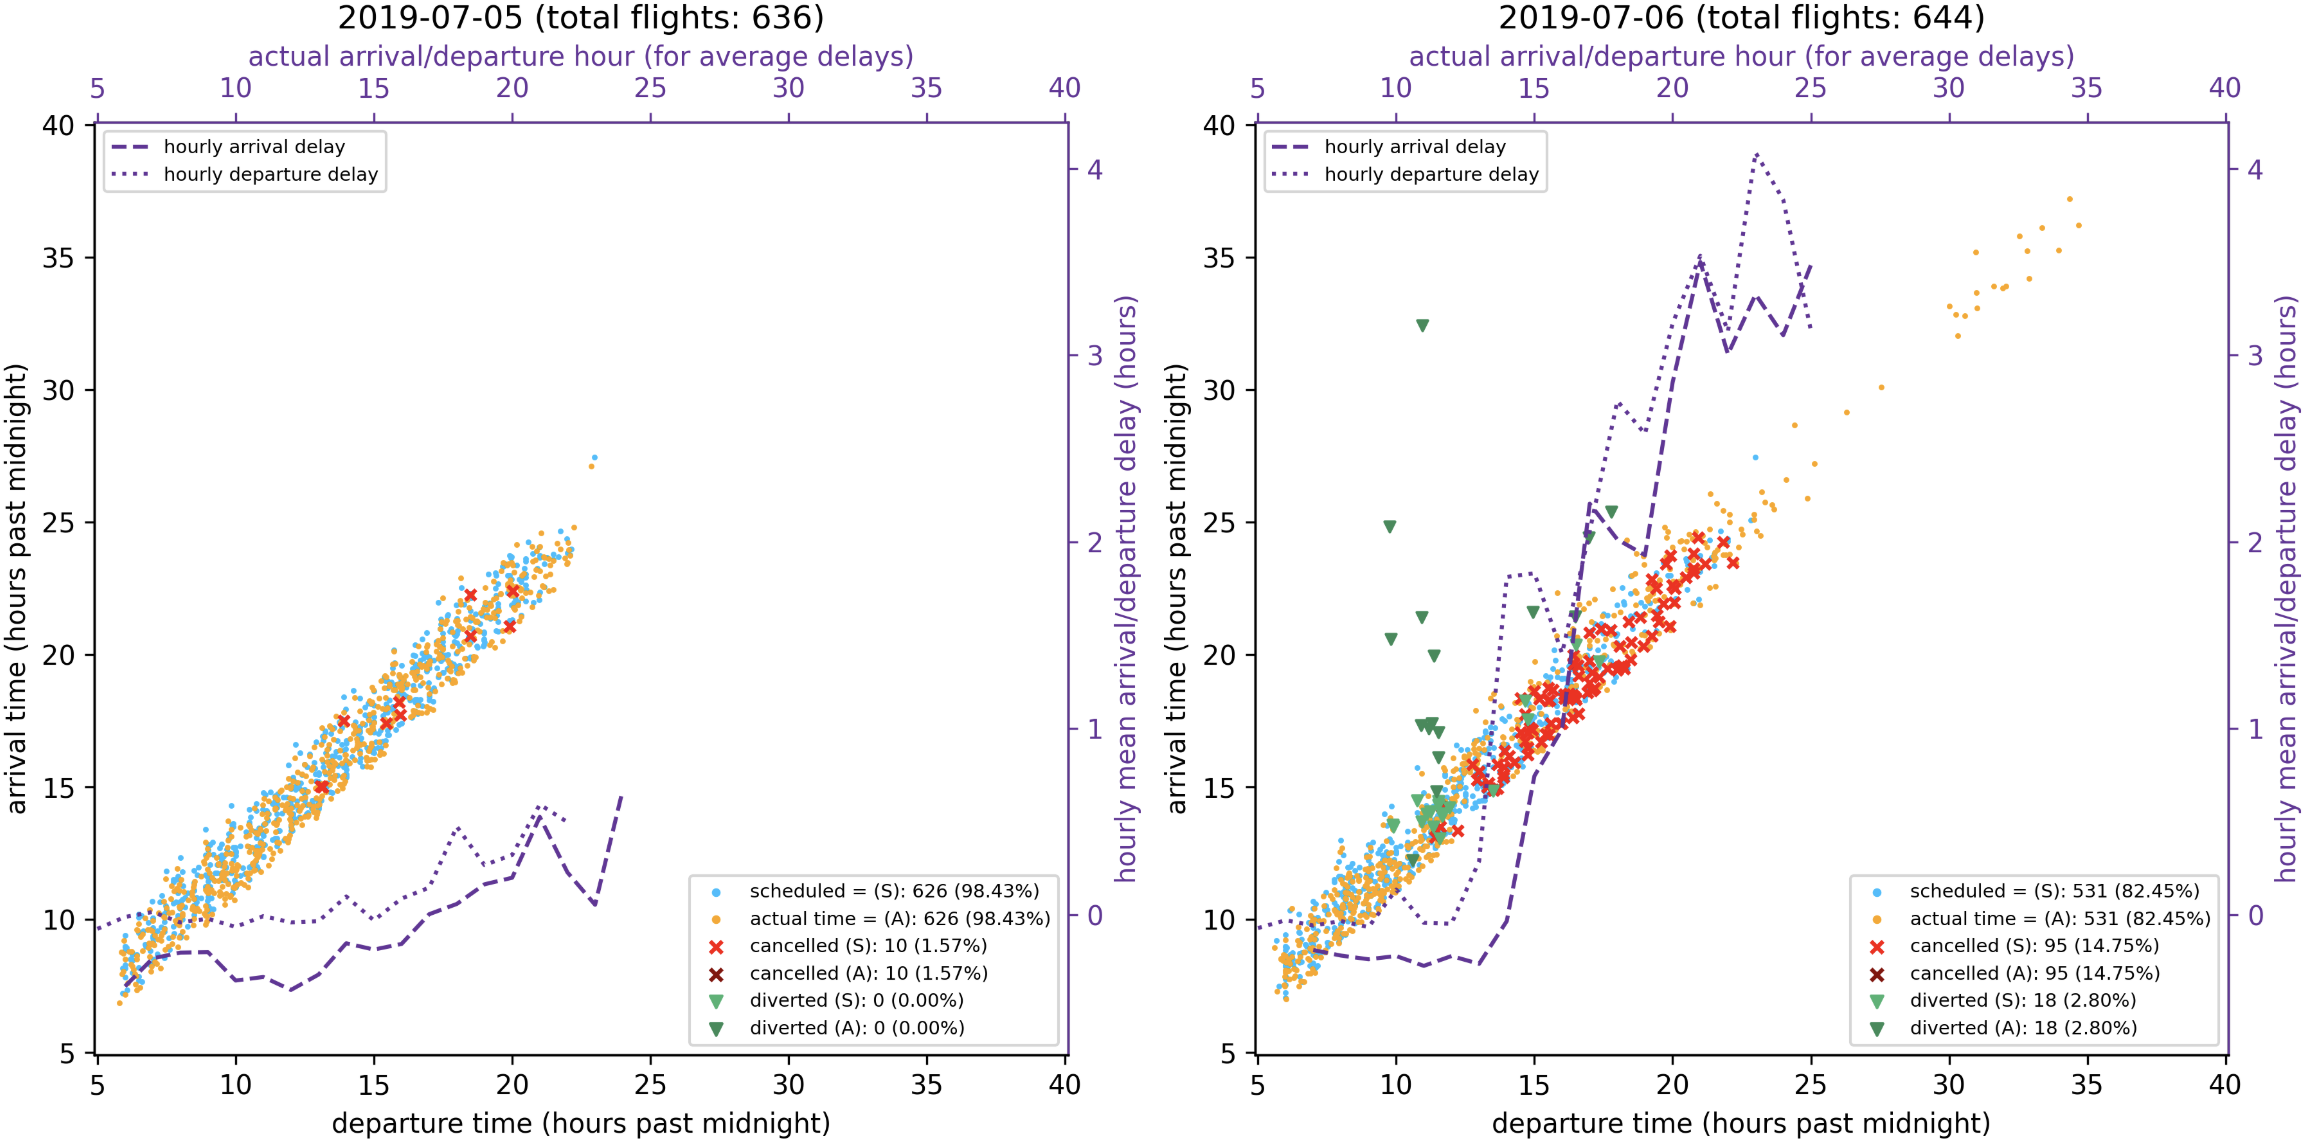
\includegraphics[width=\linewidth]{media/delay-comparison.png}
    \caption{Comparison of schedules and actual performance of flights at LGA in a day with significant delays and cancellations (right), and a day without (left). }
    \label{fig:delay-comparison}
\end{figure}

Other responses may be preemptive, in response to potential disruptions from weather events, implemented through Traffic Management Initiatives (TMI) \cite{jones_risk-adjusted_2023}. These often involve Traffic Flow Management System (TFMS) programs, which include ground delay programs (GDP), airspace flow programs (AFP), and collaborative trajectory options programs (CTOP). These programs can also have effects that span across the network, instead of just being localized at a single node. For example, in GDPs, aircraft are held on the ground at the origin airport of flights to help manage incoming demand at specific locations, eagerly shifting the delays to waiting on the ground rather than lazily accumulating flights in airborne holding, a less desirable position \cite{faa_tmi_2024}.

In particular, we can see the natural hierarchical structure to the problem, because the relationship between weather and delays is not always perfectly straightforward. However, the relationship between weather and certain intermediate factors, such as the aforementioned TMIs, and the relationship between those intermediate factors and observed delays, are more well-defined, and give us some structure work with.


\section{Posterior Approximation}
\label{background-approximate-inference}

In this and the following part, we will consider a simple model involving $\rx$ and $\rz$, where $\rx$ is observed and $\rz$ is a latent parameter. Given observations $x\in \Data$, we are often interested in inferring the posterior distribution of the latent parameters. Unfortunately, this posterior is often computationally intractable. To see why, suppose that we have $\pld{x\given z}$ as our model, and some prior $\pd{z}$. Then by applying Bayes' rule, we have
\begin{equation}
    \pld{z\given x} = \frac{\pld{x\given z}\pd{z}}{\pld{x}},
\end{equation}
where the marginal in the denominator is generally intractable as it requires computing
\begin{equation}
    \pld{x} = \int \pld{x\given z}\pd{z} \,dz.
\end{equation}
Instead, it is often more practical to approximate this posterior instead, using methods such as Laplace's approximation \cite{laplace1776}, or variational inference \cite{blei2017variational}, for example. In cases where the likelihoods aren't available either, there are other families of methods such as Markov Chain Monte Carlo (MCMC) \cite{metropolis_1953}, or Approximate Bayesian Computation (ABC) \cite{abc_2013} that can be used. We discuss these further in \cref{ch:lit-review}.


\section{Variational Inference}
\label{background-variational-inference}

We briefly introduce the concepts behind variational inference \cite{blei2017variational}, as background because we will be applying it heavily in \cref{sec:atrds-theory}. Returning to the problem formulation in \cref{background-approximate-inference}, we also suppose $\rx$ and $\rz$ follow a true distribution $\ptd{x,z}$, and we view $\pld{x,z}$ as a learned generative model parameterized by $\theta$. Our goal is then two-fold: first, we wish to find $\hat\theta$ such that $\pld{\cdot}$ serves as a good model for $\ptd{\cdot}$, which may be framed as the following maximum likelihood optimization problem:
\begin{equation}
    \hat\theta = \argmax_{\theta} \EX{\rx,\rz\sim \ptd{\cdot,\cdot}}{\pld{x,z}},
\end{equation}
and second, we would like to approximate the posterior distribution $\pld{z\given x}$. To do this, we search within a family of simpler variational distributions $\qvd{z\given x}$, parameterized by $\phi$ for a good approximation, according to some objective. For this purpose, the evidence lower bound (ELBO) is often used as an objective to maximize \cite{zhang2018advances}, given some training dataset $\Data$, which is given by
\begin{align}
    \elbo{q}{\phi, \theta, \Data}
    &= \EX{\rx \sim \ped{\cdot;\Data}}{ \EX{\rz \sim \qvd{\cdot\given x}}{\log \pld{x,z} - \log \qvd{z\given x}} }.
\end{align}

\subsection{Rewritten Likelihood Objective}
Additional, we note that the ELBO can also be written as
\begin{align}
    \elbo{q}{\phi, \theta, \Data}
    &= \EX{\rx \sim \ped{\cdot;\Data}}{ \EX{\rz \sim \qvd{\cdot\given x}}{\log \pld{x} + \log \pld{z\given x} - \log \qvd{z\given x}} }\\
    &= \EX{\rx \sim \ped{\cdot;\Data}}{\log\pld{x}} -\EX{\rx \sim \ped{\cdot;\Data}}{\EX{\rz \sim \qvd{\cdot\given x}}{ \log \frac{\qvd{z\given x}}{\pld{z\given x}}} }\\
    &= 
    -\underbrace{H(\ptd{x})}_{\text{fixed}}
    -\underbrace{\DKL{\ptd{\cdot}}{\pld{\cdot}}}_{\text{MLEO}} 
    -\underbrace{\EX{\rx \sim \ped{\cdot;\Data}}{\DKL{\pld{\cdot\given x}}{\qvd{\cdot\given x}}}}_{\text{PMO}},
\end{align}
which makes the division of the ELBO into a fixed term, an maximum likelihood estimation objective (MLEO) term, and a posterior matching objective (PMO) term explicit \cite{yacoby2020failure}. Here, we can see that maximizing the ELBO is equivalent to minimizing the KL-divergences between $\ptd{x}$ and $\pld{x}$, and $\pld{z\given x}$ and $\qvd{z\given x}$, so we want
\begin{equation}
    \hat\phi,\hat\theta = \argmax_{\phi,\theta} \elbo{q}{\phi,\theta, \Data}.
\end{equation}

\section{Normalizing Flows}

Normalizing flows are often used as an expressive variational family, as they are much more flexible in terms of the types of distributions they can approximate closely, compared to, say, a multivariate Gaussian. They start from a simple base distribution $q$, typically a normal distribution, and apply a smooth invertible function $f_\phi$ to link the simple base distribution with a presumably more complex target distribution \cite{rezende2016variationalinferencenormalizingflows}. One advantage is that exact likelihoods are available, as they can simply be calculated as 
\begin{equation}
    \log q_\phi(z) = \log q\left(f_\phi^{-1}(z)\right) -\log\left|\det J_{f_\phi}\left(f_\phi^{-1}(z)\right)\right|,
\end{equation}
where $J_{f_\phi}$ denotes the Jacobian of $f_\phi$ \cite{Kobyzev_2021}. Developments in new architectures, through different choices and parameterizations of $f_\phi$, faster and more effective ways to train normalizing flows, and further generalizations have been an active area of research \cite{onken2021otflowfastaccuratecontinuous, lipman2023flowmatchinggenerativemodeling, holderrieth2025generatormatchinggenerativemodeling}.

\chapter{Literature Review}
\label{ch:lit-review}

We present a brief overview of related work, which can be roughly divided into two parts. The first is methods pertaining to the statistical aspect of our problem, and the second is methods specifically focused on the air traffic problem, and some other potential applications with similar structure.

\section{Rare Event Analysis}

There has been much work in failure prediction and sampling in simulation, such as \cite{pmlr-v211-delecki23a} and \cite{pmlr-v229-dawson23a}, which frame learning the distribution of failure trajectories as an approximate Bayesian inference problem and leverage differentiable simulation for faster convergence, as well as without simulation, such as \cite{Asghar2024EfficientRE}, which uses unsupervised normalizing flows to enhance Monte Carlo sampling. 

While there has been less done in rare event modeling so far, one important work that is particularly relevant to the work in this proposal is \cite{dawson2025rare}, in which Dawson et al. develop a self-regularized normalizing flows framework for learning failure posteriors, which builds upon the ideas of prior regularization \cite{abdollahzadeh2023surveygenerativemodelinglimited} and bootstrapping. Specifically, they allow the nominal data to help regularize the limited failure data and develop a bootstrapping inspired approach to share information between the learned model components, to mitigate overfitting. 

\section{Generative Modeling}
\label{related-generative-modeling}

Architectures for generative models have grown in popularity in recent years, such as variational autoencoders (VAEs) \cite{kingma2022autoencodingvariationalbayes,li2024deep, chevrot2022cae}, normalizing flows \cite{papamakarios2021normalizing}, and diffusion models \cite{yang2023diffusion}, and have been utilized across various domains with complex data such as image generation \cite{doersch2016tutorial}, biology \cite{guo2023diffusionmodelsbioinformaticsnew}, and autonomous systems \cite{xu2023diffscene}. Generative modeling has also been applied to learn approximate failure distributions from observations \cite{yue2023gan,pinto2023deep}. However, discussed in \cref{subsec:intro-latent-artificial}, these techniques have some limitations that may be untenable in our use case, as they require a large amount of data for training, and lack physical interpretability in their latent spaces. Because of this, we first more directly leverage variational inference \cite{hoffman2013stochastic} in our proof of concept.


\section{Using Domain Knowledge}
\label{related-sbi}

As discussed in \cref{subsec:intro-latent-natural}, carefully constructing the latent space based on domain can be helpful in building the overall model. Simulation-based Inference (SBI) is a related field, which develop methods to incorporate information from simulations of the underlying dynamics into statistical inference techniques \cite{cramer_sbi_2020, gloeckler2024allinonesimulationbasedinference}. These focus mainly on likelihood-free methods, to accommodate a wider range of distributions. Similarly, physics-informed learning develops methods to integrate knowledge of physical laws as partial differential equations (PDEs) for the problem at hand into the learning process \cite{hao2023physicsinformedmachinelearningsurvey, Karniadakis_Kevrekidis_Lu_Perdikaris_Wang_Yang_2021}. Both of these types of methods follow the same goal as in our case, where we wish to use domain knowledge about the underlying distribution of our dataset which is not evident from just looking at the data itself.


\section{Air Traffic Applications}

While not comprehensive, we also discuss some prior work specific to the air traffic problem, to understand the gap we are trying to fill with our work. Most prior work focuses on individual parts of the problem, such as modeling the impact of weather on GDPs using support vector machines (SVM) and logistic regression \cite{liu_modeling_2020}, or predicting the impact of weather on air traffic flow using a multi-modal long short-term memory (LSTM) attention-based network \cite{ZENG2024102935}. On the traffic network side, much work has been done in developing simulations, such as \cite{PYRGIOTIS201360}, though most are not differentiable and do not have likelihoods. We also differ in that we are working with the whole model together, and in that we use Bayesian methods, so that we also have all of those associated benefits, such as having uncertainty quantification built in. While there has also been work for modeling everything from weather to the observed outcome and factors in between, such as \cite{enea_analysis_2024} and \cite{reitmann_advanced_2019}, these similarly do not allow us to easily learn posteriors or build a generative model that can be leveraged for other goals.


\section{Related Applications}
\label{related-applications}

For completeness, we also list a few alternative problems that can be modified to fit a similar hierarchical structure to that of the air traffic weather problem, if they do not already. These have simulations available, which we can also attempt to re-implement as a differentiable probabilistic program, if desired, or apply likelihood-free methods to. Many of these models are also simpler to implement than the air traffic model, and have been well studied separately, so they may be easier to evaluate techniques with as an initial step. These alternative applications include parameterizing gravitational wave population \cite{ruhe2022normalizingflowshierarchicalbayesian}, seismic waveform inversion \cite{gouveia1998swi}, spread of infectious diseases \cite{trostle2022gaussianprocessapproximationspatialsir}, and calibrating stochastic radio channel propagation models \cite{bharti2022radio}.



\chapter{Guiding Case Study: LaGuardia}
\label{ch:atrds}

This chapter will contain the primary technical contribution of the thesis. Here, we will perform a guiding case study that will serve as both a proof of concept and motivation for further directions of study, which will we begin to explore in \cref{app:atm}, \cref{app:risk}, and \cref{app:shrinkage}. It is also important to note that it is a simplified proof of concept that may seem over-complicated at first, for the simple scenario. However, this is done intentionally to show how we would develop more complex methods for this use case, which may be necessary background for future work such as moving our problem up from tabular weather data to weather image or video generation.

\section{Overview}

As a proof of concept for the general proposed study, we consider a simplified model of the relationship between weather and delays at LaGuardia Airport (LGA), and provide a demonstration of simultaneously inferring the posterior distribution of the latent parameters and fitting our model to historical data. We use stochastic variational inference (SVI), as introduced in \cref{background-variational-inference}, to learn an approximation for the posterior, and develop a simple form of amortized inference to demonstrate how it can be used for failure prediction and test case generation. 

\section{Single Airport Problem}
\label{sec:atrds-single-airport}
To motivate the decisions made in our simplified model, we first perform an initial analysis of our empirical data. We will be focusing on the mean service time as our latent variable $\rz$, which is inversely related to airport capacity, or maximum throughput of arrival and departure events, and work on the timescale of a full day for the granularity of $\rz$ and $\rw$, i.e. we only have a single value for each day. Here, we will be assuming that we have a fully specified model for the $\pld{x\given z;y}$ component, but still need to learn $\pld{z\given w}$, which we will do at the same time as learning the relevant posteriors.

\subsection{Flight Data}
Scheduled and actual flight times are taken from the Bureau of Transportation Statistics (BTS) Reporting Carrier On-Time Performance database \cite{bts_transstats_nodate}. Flights from the years 2018 and 2019 are used for training, but analysis is focused on July 2019. Specifically, for each flight in a day, we take the scheduled departure and arrival times for the context $y$, and the actual times for observations $x$, where times are converted to hours past midnight in LGA local time. We restrict our focus to modeling accumulated delays throughout the day, so we do not make additional provisions for cancellations or diversions.

Later, in \cref{sec:atrds-theory}, we will also need to use a coarser encoding of $x$ and $y$ on the same timescale as $z$ and $w$. For this, we will define our aggregation for $x$ as the straight average across all flights in the day, where flights that arrive early are considered as having zero delay instead of negative delay. We will aggregate $y$ by counting the number of operations scheduled in each hour of the day, and taking the maximum, as shown in \cref{fig:split-scheduled-capacity}. We also tried using the total number of flights in the day as a measure of aggregate scheduled demand, and obtained similar results.

\begin{figure}[htb!]
    \centering
    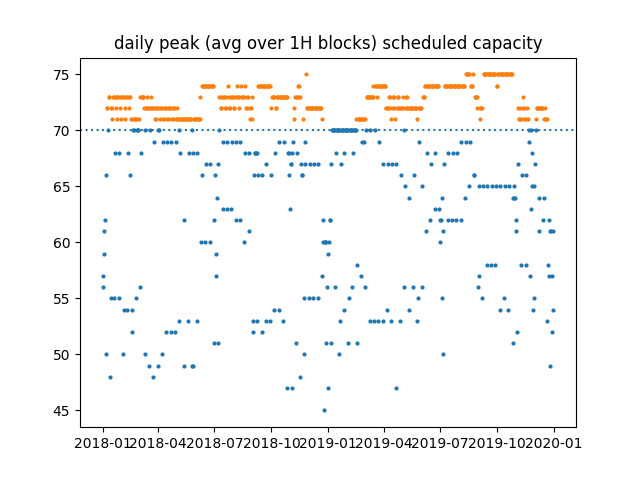
\includegraphics[width=0.8\linewidth]{media/lga-analysis-14.png}
    \caption{Daily peak scheduled hourly demand in 2018 and 2019, in operations per hour.}
    \label{fig:split-scheduled-capacity}
\end{figure}

\subsection{Weather Data}
We restrict our focus to considering the impact of visibility and ceiling, as these weather conditions are known to directly affect airport capacity \cite{2014lga}. Measurements are taken from the National Oceanic and Atmospheric Administration (NOAA) Local Climatological Data Version 2 (LCDv2) dataset \cite{weatherdata}, and converted to the Meteorological Aerodrome Report (METAR) format commonly used in aviation. Specifically, visibility is already given as an hourly value, but ceiling must be inferred from provided sky condition data by taking the height of the lowest cloud layer with at least 4 oktas of coverage.

For our encoding as a daily aggregate value, we use the harmonic mean~\cite{ferger1931nature} for the sky ceiling, to reflect the greater relevance of lower values, and similarly select the daily minimum for the visibility. We clip values at $10000$ feet and $10$ statute miles for ceiling and visibility respectively, for numerical stability, and because there is not really any meaningful difference among higher values.


\subsection{Initial Motivating Analysis}

To see why our choice of variables is well motivated for a proof of concept study, we examine the relationship between weather and delays, which our learned model should be able to reflect, if it is a good representation. First, we note that lower ceilings and visibilities appear to partially coincide with days with higher delays, as shown in \cref{fig:2019-07-weather-delay-timeline}.

\begin{figure}[htb!]
    \centering
    % 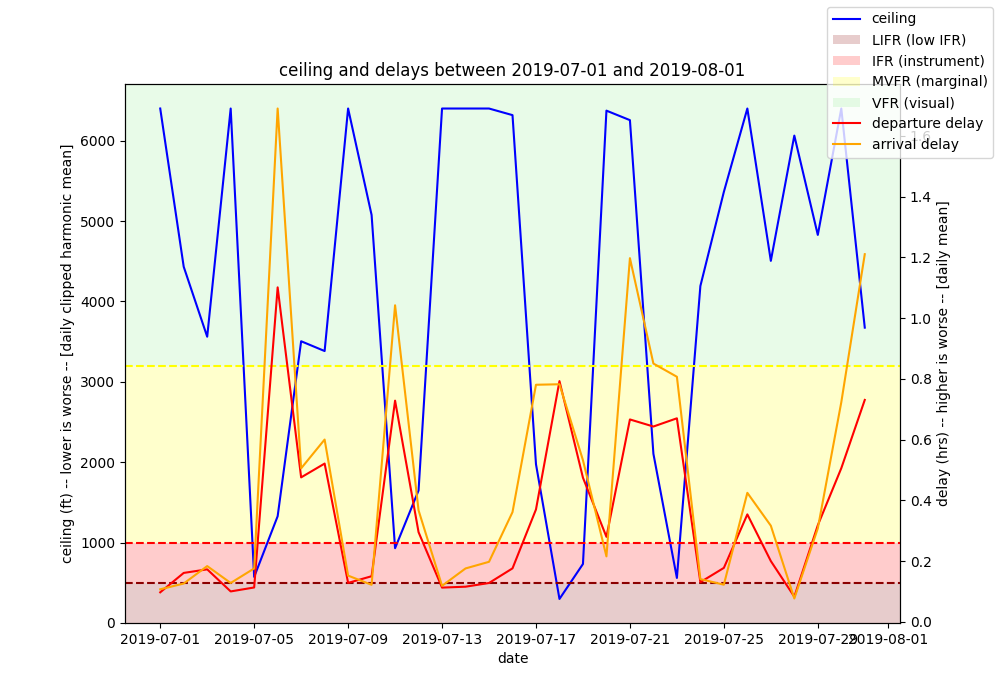
\includegraphics[height=5.5cm]{media/lga-analysis-1.png}
    % 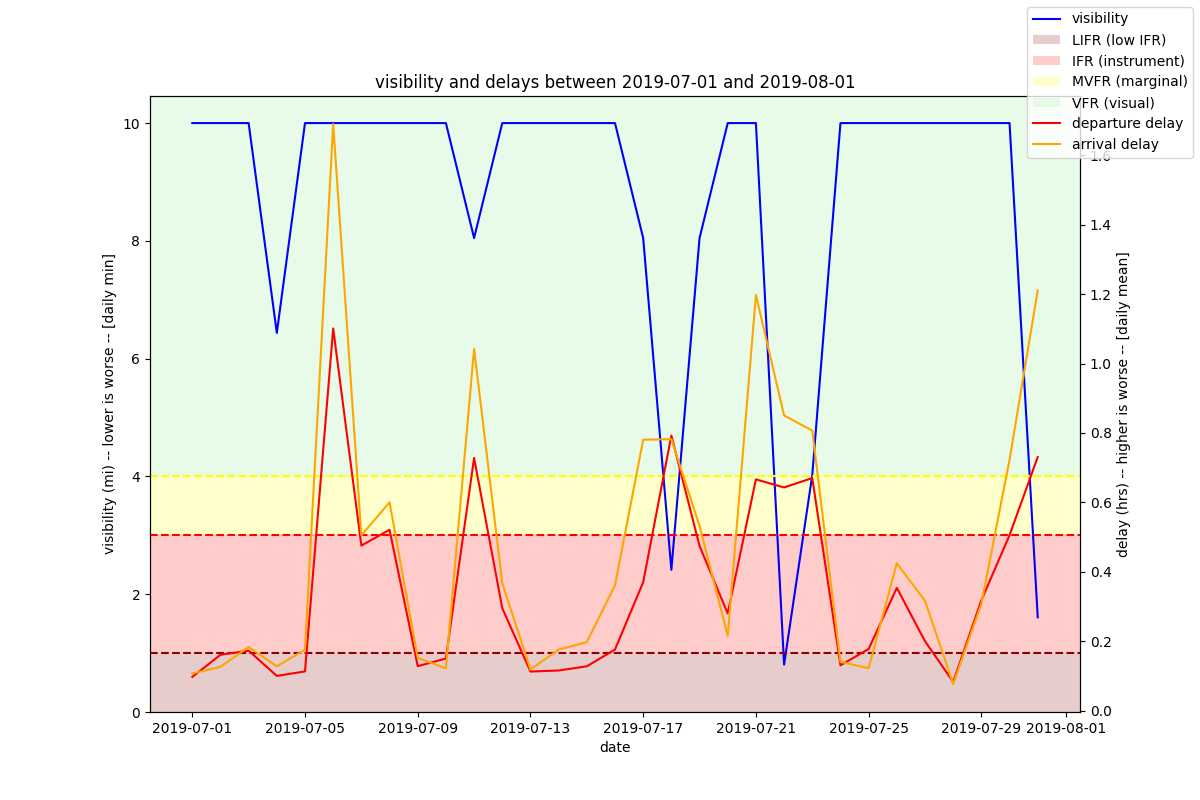
\includegraphics[height=5.5cm]{media/lga-analysis-3.png}
    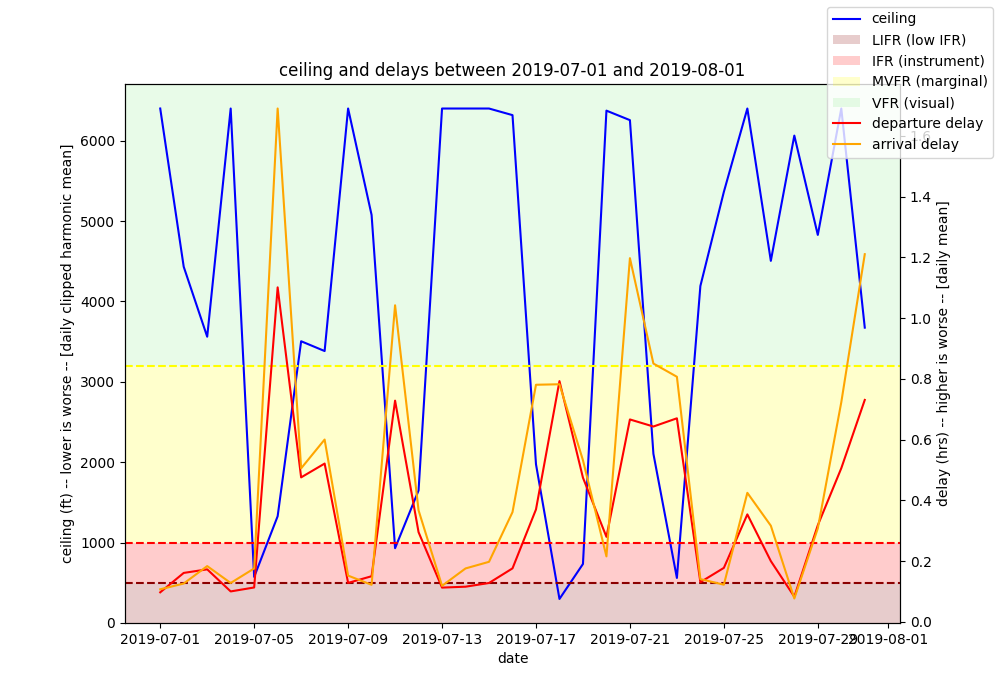
\includegraphics[width=.66\linewidth]{media/lga-analysis-1.png}
    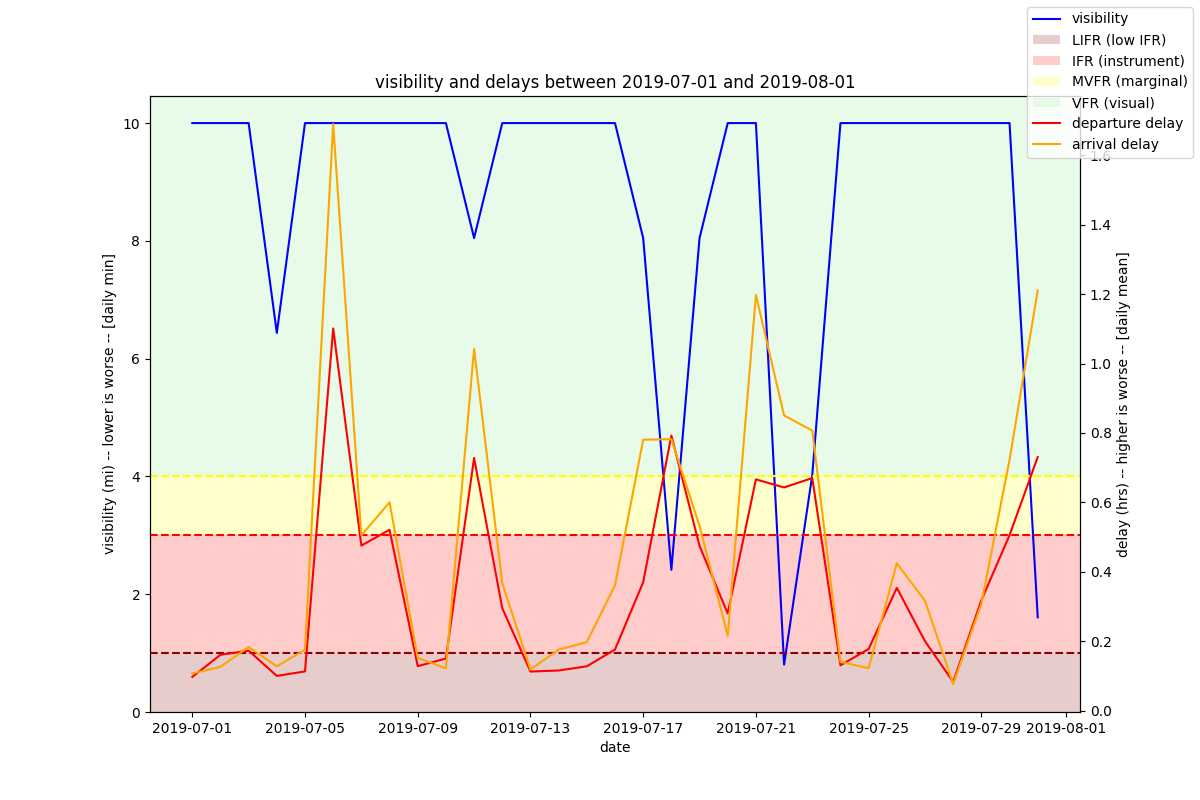
\includegraphics[width=.66\linewidth]{media/lga-analysis-3.png}
    \caption{Timeline of ceiling (upper) and visibility (lower) compared to delays in July 2019. Days with poorer weather, where the blue line is lower, coincide with days with greater delays, where the red and orange lines are higher. Flight rule regions show severity of weather.}
    \label{fig:2019-07-weather-delay-timeline}
\end{figure}

\begin{figure}[htb!]
    \centering
    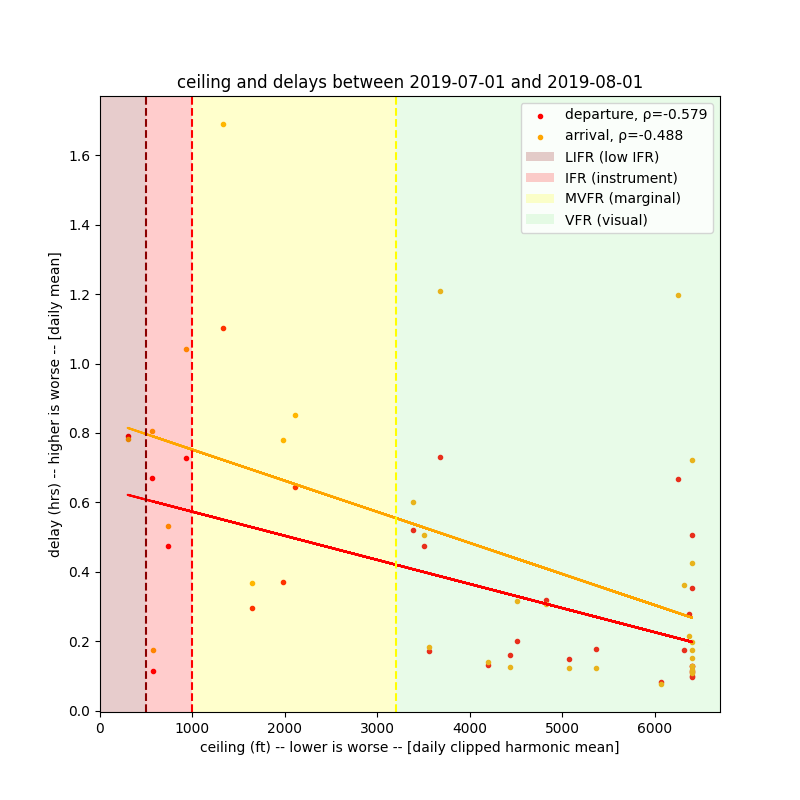
\includegraphics[height=8.1cm]{media/lga-analysis-2.png}
    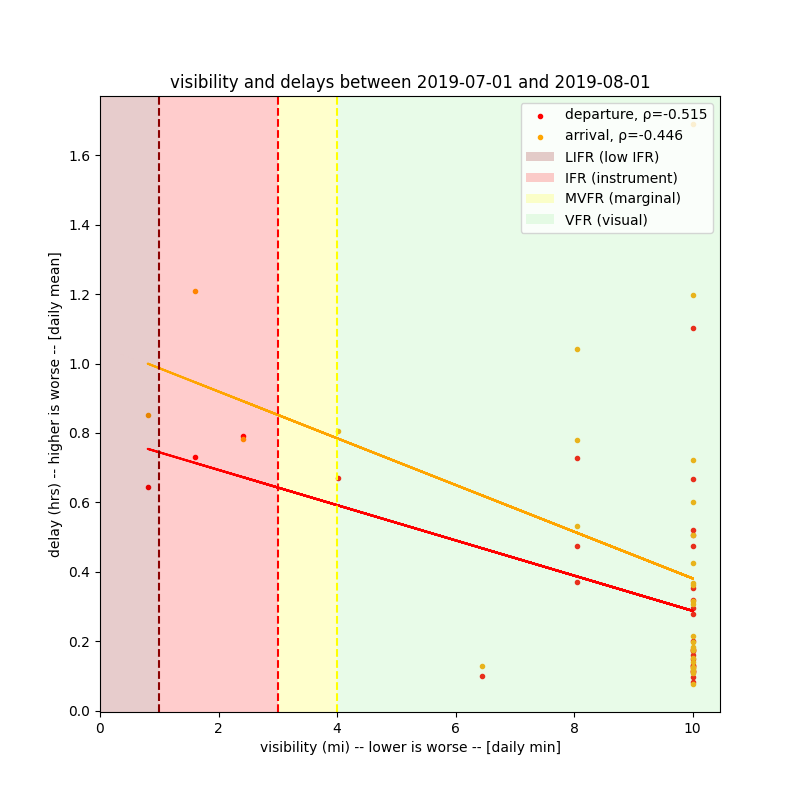
\includegraphics[height=8.1cm]{media/lga-analysis-4.png}
    \caption{Scatter plot of ceiling (left) and visibility (right) compared to delays in July 2019.}
    \label{fig:2019-07-weather-delay-scatter}
\end{figure}

Here, instrument flight rule (IFR) weather conditions are supposed to lead to a lower maximum throughput, meaning likely higher delays, than visual flight rule (VFR) conditions, which appears to align well with what we observe. To make this relationship a bit more obvious, we also show the same data in the timeline as a scatter plot with trend line and Pearson correlation coefficient, in \cref{fig:2019-07-weather-delay-scatter}. 


It is important to re-iterate, however, that weather is not the only factor that is considered in modeling delays, as is emphasized in \cref{fig:bubble3d-all}. We can see that higher scheduled capacity, corresponding to busier days, are more prone to delays at the same weather conditions compared to a lighter day, for example. This distinction in distribution of delays given weather is illustrated in \cref{fig:bubble2d-split}, which is essentially a 2D top view of an upper and lower partition of the full 3D plot.

\begin{figure}[htb!]
    \centering
    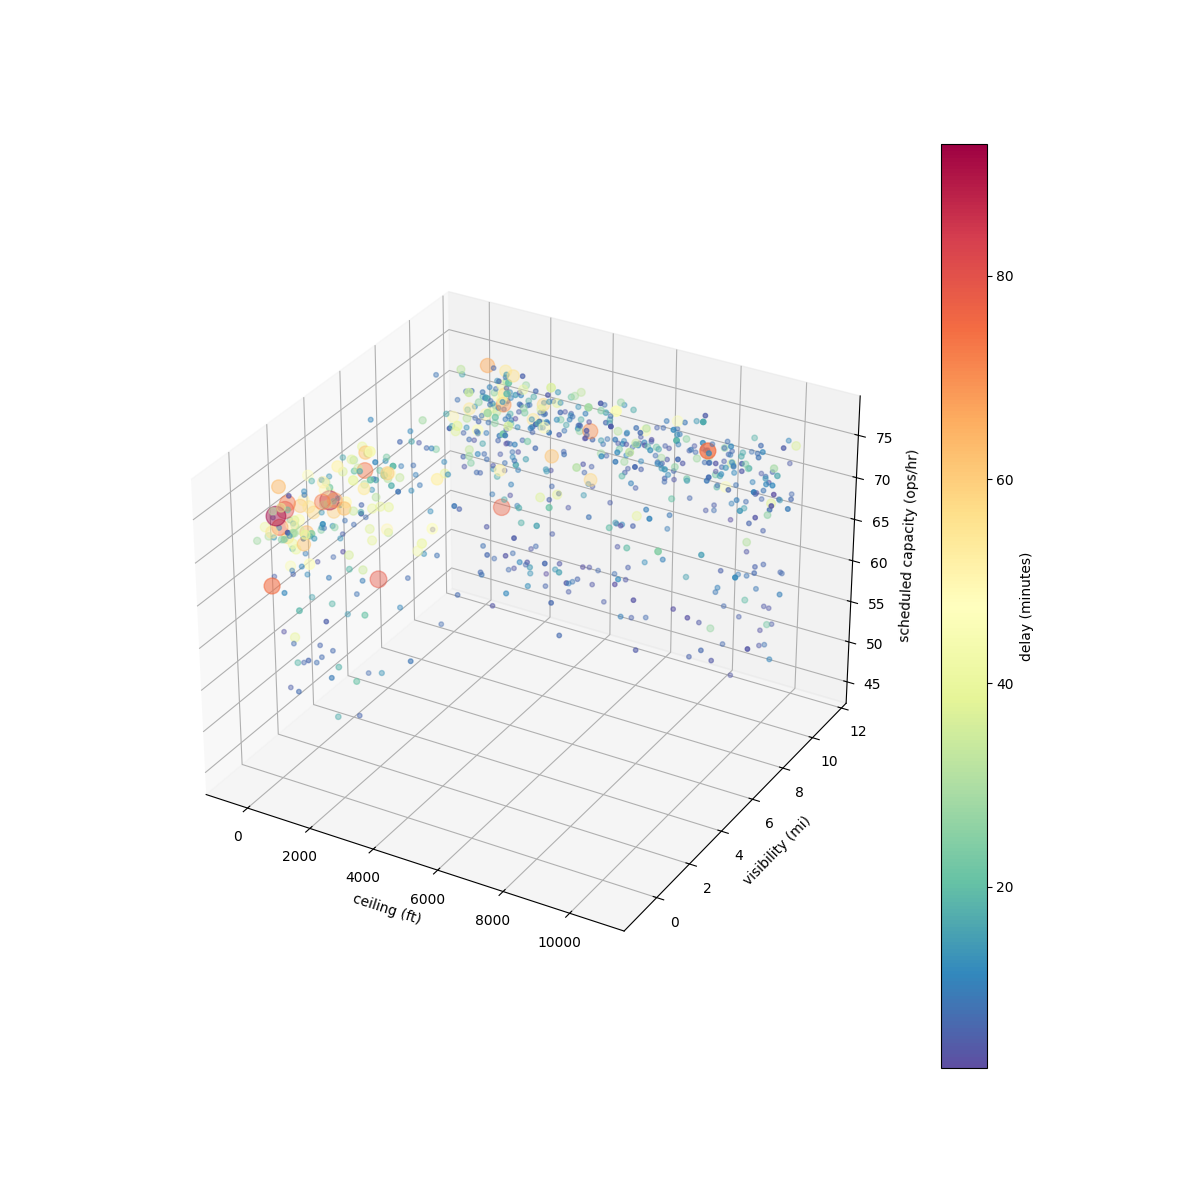
\includegraphics[width=\linewidth]{media/lga-analysis-17.png}
    \caption{3D scatter plot of both weather conditions and scheduled demand for each day in 2018 and 2019, where delay is represented with color. Points with higher delay also have greater size and opacity, for emphasis, and some noise is added for visualization purposes. }
    \label{fig:bubble3d-all}
\end{figure}

\begin{figure}[htb!]
    \centering
    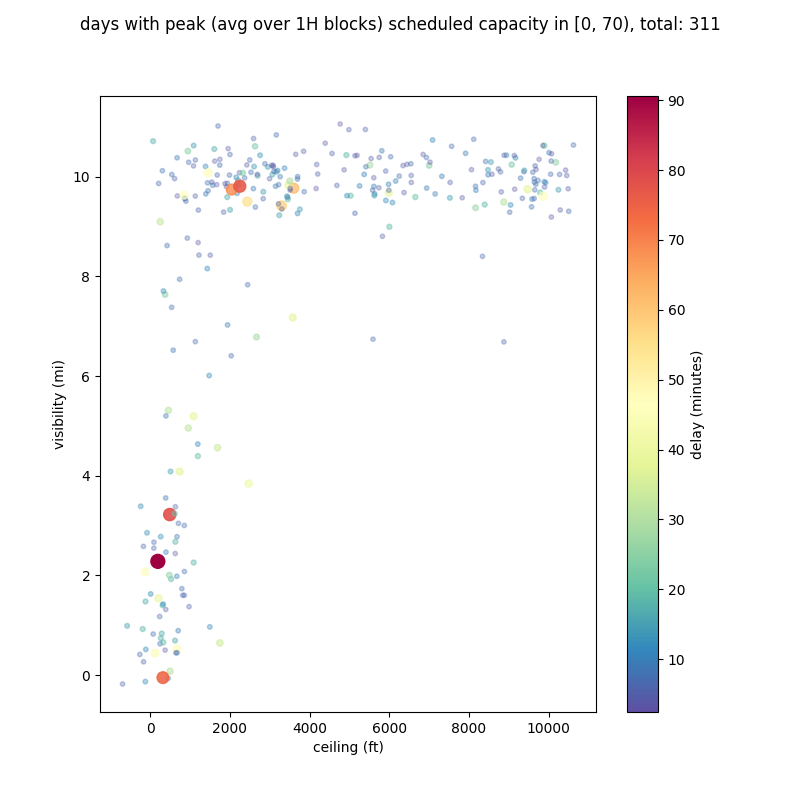
\includegraphics[height=8.0cm]{media/lga-analysis-15.png}
    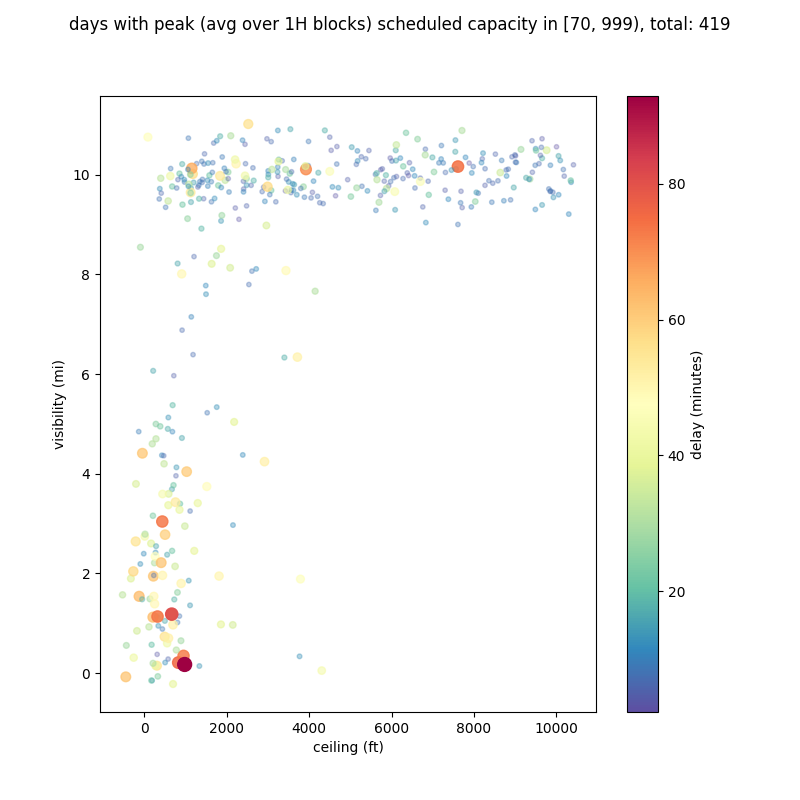
\includegraphics[height=8.0cm]{media/lga-analysis-16.png}
    \caption{Different distributions of delays given weather for lighter (left) and busier (right) days, which shows that failures are more concentrated in the region of higher demand and worse weather.}
    \label{fig:bubble2d-split}
\end{figure}

\subsection{Stochastic Airport Simulation}

We extend and adapt the stochastic queuing model developed in \cite{dawson2024breaking, michael_peng_probing_2024}, which was originally developed to study the mass cancellations and delays during the 2022 Southwest Airlines winter weather crisis, to better support our particular use case of less severe, but still impactful weather conditions. Specifically, we make two main changes.

The first is that we extend the model to be closer to reality, in terms of flights included. The original model only includes flights that have both endpoints, i.e. arrival and departure airport, within the set of 4 to 10 key network airports included. Additionally, only flights operated by Southwest are tracked. We add support for including all airline carriers present in the schedule data simultaneously, and also implement tracking for flights with one endpoint outside of the network. This is done by adding a source supernode, which emits all flights originating from outside the network to the relevant airports, and a sink supernode, to which all flights headed outside of the network are directed. The departure times at which flights are emitted from the source node are considered exogenous variables taken directly from the context, and we support a wide range of options including both scheduled and actual times. For this study, we choose to use the actual times, so that delays that are mainly attributable to LGA are properly modeled, and so that the demand profile of incoming flights when fitting our model is as realistic as possible.

The second change is that we add support for additional types of flight failures. The original simulation models delays and eager cancellations that result from when there are not enough available aircraft at an airport to depart at the scheduled time. We extend this to also model lazy cancellations, where flights that have been waiting to depart for long enough are canceled. Analogously, flights that have been waiting to arrive, which corresponds to waiting in holding patterns, are also considered failed after a given amount of time, because it is unrealistic for flights to wait for arrivals indefinitely. For this proof of concept, however, we disable both of these features, as minimal impact was observed in the very simplified scenario. Similarly, the actions taken, i.e. deciding which flights and when to cancel or delay, is set to the simple default strategy of first in first out (FIFO), but in future work, incorporating choice of strategy into the simulation will be important, as the end goal is stress-testing future design decisions.

With this in mind, our simulation roughly proceeds as follows. Flights are emitted from the source supernode at given times, to represent external incoming demand. The ego airport, which in this case is LGA, also has departing flights it must attempt to accommodate. When flights are ready to depart or arrive at the ego airport, they are entered into a service queue to await processing. We use a single M/M/1 queue for this, where a single server handles all flights regardless of their arrival or departure status. The time between arrivals and departures is drawn from an exponential distribution, where the mean $\lambda^{-1}$ is the latent mean service time parameter. This simulates a Poisson process with rate $\lambda$, which explains the connection between our introduced mean service time and the more commonly seen airport capacity or throughput. Roughly speaking, higher mean service times can lead to increased delays if severe enough, because it will mean that the airport may become unable to handle the demand of scheduled flights and must cancel or delay some in order to operate within its current limits. We also note that this service time is meant to encompass all factors that might affect throughput at a single airport, and not necessarily just the impact from visual versus instrument flight rules.

In this simplified setting, we directly bake in the notion of the action $\ra$ into the simulation, so we make no attempt to learn it implicitly. Similarly, we do not have any learned process parameters $\theta$ that are relevant to $\pld{x\given z;y}$, as we assume that we are working with a fully specified simulator. This is also implemented as a model through Pyro, a probabilistic programming language \cite{bingham2019pyro}, which makes the simulation differentiable, and gives us access to the likelihoods, so that we can use stochastic variational inference methods directly.

It is also important to reiterate here that mean service time on its own is not the only factor relevant to delays. \cref{fig:busy-light-comparison} shows two days that did not have significant delays in reality, after artificially imposing a higher mean service time of $0.2$ hours on both and simulating the result, and observing that the busier day was hit harder. This makes sense intuitively as well, because we would expect it to be easier to recover from a disruption with less external stress, so we can expect lighter days to be more tolerant to higher service times.

\begin{figure}[htb!]
    \centering
    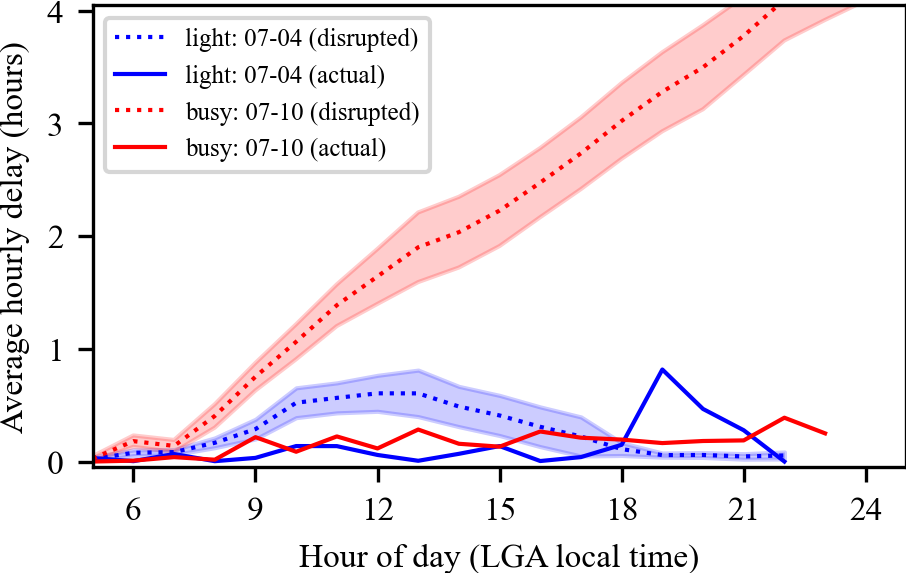
\includegraphics[width=0.7\linewidth]{media/busy_light_comparison.png}
    \caption{Demonstration of the effect of scheduled demand on delays on days with similar actual outcomes (solid lines). The same simulated disruption is applied to two days (dotted lines, shaded is standard deviation), showing that the lighter day (blue) is less affected than the busier (red).}
    \label{fig:busy-light-comparison}
\end{figure}

\subsection{Weather-Informed Priors}

We partially specify a simple mixture density model for the $\pld{z\given w}$ component. Specifically, we define a function $\fvn: w\mapsto c$ parameterized by $\nu$, where $c\in \ms C = \{0,1\}$ represents nominal and failure weather. 
\begin{proposition}[Weather Mixture Density Model]
    Then, we define our model as the following:
    \begin{equation}
        \pld{z\given w} = \begin{cases}
            \mt N(z;\mu_0, \sigma_0^2) \quad \text{if }\fvd{w} = 0\\
            \mt N(z;\mu_1, \sigma_1^2) \quad \text{if }\fvd{w} = 1,
        \end{cases}
    \end{equation}
    where $\mt N(\cdot;\mu,\sigma^2)$ denotes the univariate normal density with mean $\mu$ and variance $\sigma^2$.
\end{proposition}

We judgmentally select $\mu_0 = 0.012$ and $\sigma_0 = 0.001$ for nominal weather, and $\mu_1 = 0.019$ and $\sigma_1 = 0.001$ for failure weather, to incorporate the belief that worse weather leads to higher service times. 

\begin{proposition}[Relaxation of Threshold Classification for $\fvn$]
    For the decision function $\fvn$, we use a simple threshold classification given by
    \begin{align}
        \fvd{w} & = 1 - \sigma\left(\alpha (w_v-\wthvf)\right)\cdot \sigma\left(\alpha (w_c-\wthcf )\right) \\
        &\approx \begin{cases}
            1 \;\; \text{if} \;\; w_v \leq \wthvf \;\; \text{or}\;\;  w_c \leq \wthcf \\
            0 \;\; \text{otherwise}
        \end{cases}
    \end{align}
    where $\sigma(x)=(1+e^{x})^{-1}$ is the sigmoid function, and $\alpha = 50$ is a fixed scaling parameter to control the sharpness of the threshold.
\end{proposition}


Here, we let $w = (w_v, w_c) $, to represent the individual visibility and ceiling components, and let $\nu = (\wthvf,\wthcf)$ be thresholds parameterizing $\fvn$ that must be learned. We can interpret this model as imposing weather-informed priors on $z$ based on $w$, instead of just assuming the same prior for all observations, to incorporate the effect of weather. Additionally, we can extend this to the continuous case $\ms C=[0,1]$ directly by linearly interpolating between the nominal and failure density accordingly, as we will use in \cref{sec:atrds-theory}.

While we chose to specify all $\mu_c$ and $\sigma_c$, we also note that these can be set to different values, to investigate what the learned thresholds might be to decide between various severity levels of service time impact. 

\section{Toy Example -- Two Moons}
\label{sec:atrds-moons}
Before we move on, we present a simple toy example on the classic two moons dataset, which we augment with a weather-analogue variable. Here, we set $w\in [0,1]$, where being below a given threshold generates the nominal distribution of points in 2D space
\[
    \theta \sim \mt U(0, \pi),\quad \rx \sim\mt N(\cos\theta - 0.5, 0.1), \quad \ry \sim \mt N(\sin \theta - 0.25, 0.1)
\]
and being above the threshold generates the failure distribution from
\[
    \theta \sim \mt U(\pi, 2\pi),\quad \rx \sim\mt N(\cos\theta + 0.5, 0.1), \quad \ry \sim \mt N(\sin \theta + 0.75, 0.1),
\]
in the same way as \cite{dawson2025rare}, where $\mt U$ denotes the uniform distribution. We consider the actual point here to be the latent variable $z$, and add Gaussian noise to it to obtain observations $x$. Then, we attempt to learn an approximation for the posterior $\pld{z\given x,w}$, for each range of $w$, failure and nominal.

\begin{figure}[htb!]
    \centering
    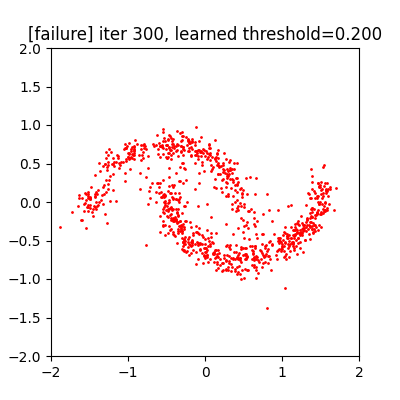
\includegraphics[height=7.5cm]{media/Figure_1A.300.png}
    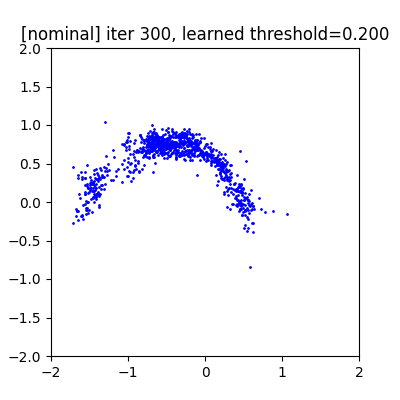
\includegraphics[height=7.5cm]{media/Figure_2A.300.png}
    \caption{Samples from two moons learned posteriors, with incorrectly specified threshold.}
    \label{fig:2moons-bad}
\end{figure}

\begin{figure}[htb!]
    \centering
    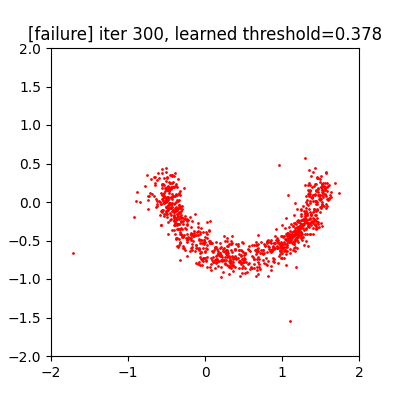
\includegraphics[height=7.5cm]{media/Figure_1.300.png}
    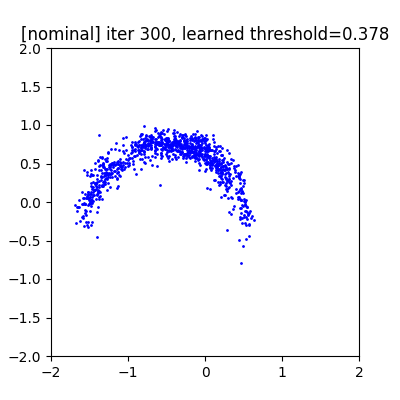
\includegraphics[height=7.5cm]{media/Figure_2.300.png}
    \caption{Samples from two moons learned posteriors, with correct learned threshold.}
    \label{fig:2moons-good}
\end{figure}

\cref{fig:2moons-bad} shows the result when the threshold is incorrectly specified, and \cref{fig:2moons-good} shows the result when the threshold is simultaneously learned. Here, we use a normalizing flows architecture to learn posteriors. As we can see, it is important to ensure that that if we are learning separate posteriors, that they are primarily learned on the data that we are interested in. In the case of the air traffic problem, it is part of the reason why it can be problematic to just classify days into failure or nominal purely based on observed delay or weather, because if our classification is wrong or we do not yet have a clear understanding of how those relate to different regions of the latent space, we may obtain inaccurate or less useful results.

\section{Theoretical Development}
\label{sec:atrds-theory}
\begin{figure} [htb!]
    \centering
    % feel free to improve this i don't actually know how to use this
    \tikz{
        % nodes
        \node[obs] (y) {$\rx$};%
        \node[latent,left=of y, xshift=-.4cm] (z) {$\rz$} ; %
        \node[obs,left=of z, xshift=-.4cm] (w) {$\rw$}; %

        % Factors
        \factor[left=of y, xshift=-.2cm] {z-y} {below:$\pld{x\given z;y}$} {} {} ; %
        \factor[left=of z, xshift=-.2cm] {w-z} {below:$\pld{z\given w}$} {} {} ; %

        \factor[above=of z, yshift=.1cm] {q} {above:$\qvd{z\given x,w;y} \approx \pld{z\given x,w;y}$} {} {} ; %
        \factor[below=of z, yshift=-.1cm] {r} {below:$\rvd{w\given x;y} \approx \pld{x\given w;y}$} {} {} ; %

        \node[const,above=of y, yshift=-.42cm] (y_above) {} ;
        \node[const,below=of y, yshift=.42cm] (y_below) {} ;
        \node[const,above=of w, yshift=-.42cm] (w_above) {} ;
        \node[const,below=of w, yshift=.42cm] (w_below) {} ;
        
        % % plate
        % \plate [inner sep=.25cm,yshift=.2cm] {plate1} {(x)(y)(z)} {$N$}; %
        % edges
        % \edge {w} {wt} ;
        % \edge {wt} {z} ;
        % \edge {z} {y} ;

        \edge[dashed, -] {w} {w_above} ;
        \edge[dashed, -] {y} {y_above} ;
        \edge[dashed] {w_below} {w} ;
        \edge[dashed, -] {y} {y_below} ;
        
        % factor edges
        % \factoredge[densely dashdotdotted] {w} {w-wt} {wt} ; %
        % \factoredge[densely dashdotdotted] {wt} {wt-z} {z} ; %
        \factoredge {w} {w-z} {z} ; %
        \factoredge {z} {z-y} {y} ; %

        \factoredge[dashed] {w_above,y_above} {q} {z} ; %
        \factoredge[dashed,-] {y_below} {r} {w_below} ; %
    }
    \caption{Overview of the probabilistic formulation for the proof of concept, with context $\ry$ omitted for clarity, showing where each of the variational approximations fit into the overall picture.}
    \label{fig:wzx-poc}
\end{figure}


As outlined in \cref{sec:intro-variants}, we will first need to learn posterior distributions $\pld{z\given x,w;y}$, while simultaneously fitting our model to historical observations. Then, we can use this learned model to predict effects of different conditions on a new day, or learn a different conditional density of interest. To this end, we apply stochastic variational inference, as introduced in \cref{background-variational-inference}, for the same reasons of computational tractability. In \cref{fig:wzx-poc}, we outline the distributions we are attempting to approximate. 

\subsection{Cluster Labels}

We will start with learning an approximation for latent posterior distribution $\qvd{z\given x,w;y}\approx \pld{z\given x,w;y}$. As discussed in \cref{sec:atrds-single-airport}, it is difficult to immediately identify which data points to group together for accurate learning of separate posteriors, so we will also learn a way to simultaneously cluster these points into groups, in a principled way, which also effectively also makes part of our learning problem unsupervised.

For this case study, we also adopt a simple threshold-based classification model. Specifically, we also select thresholds $\xth$ and $\yth$, and define a clustering function $\gvn:(x,y,w)\mapsto (d_x,d_y,d_w)=d$ as follows, with $x'$ and $y'$ as the result from aggregating $x$ and $y$ as described in \cref{sec:atrds-single-airport}:
\begin{proposition}[Partial Relaxation of Clustering for $\gvn$]
    We define our clustering function $\gvn$ as follows:
    \begin{align}
        \gvd{x,y,w}_x = d_x &= \mbm1_{x'\ge\xth}\\
        \gvd{x,y,w}_y = d_y &= \mbm1_{y'\ge\yth}\\
        \gvd{x,y,w}_w = d_w & = 1 - \sigma\left(\alpha (w_v-\wthvg)\right)\cdot \sigma\left(\alpha (w_c-\wthcg )\right) \\
        &\approx \begin{cases}
            1 \;\; \text{if} \;\; w_v \leq \wthvg \;\; \text{or}\;\;  w_c \leq \wthcg \\
            0 \;\; \text{otherwise.}
        \end{cases}
        % \begin{cases}
        %     1 \quad\text{if }\widetilde{x} \le\xth\\
        %     0 \quad{\text{otherwise}}
        % \end{cases}
    \end{align}
\end{proposition}

Here, $\mbm1$ is an indicator that takes on value $1$ when the condition is true and $0$ otherwise, and $\sigma(\cdot)$ is the sigmoid function.We use separate thresholds for the $w$ components in $\fvn$ and $\gvn$ because it is possible that the relevant thresholds for weather are different when also introducing contributions from other variables such as $y$. Similarly to $\fvn$, we set the parametrization for $\gvn$ as $\lambda = (\wthvg, \wthcg)$. In both $\fvn$ and $\gvn$, we use a smooth approximation for the weather threshold indicator to maintain differentiability, so the relevant ranges here are $c\in\ms C=[0,1]$ and $d\in \ms D=\{0,1\}\times \{0,1\}\times [0,1]$, where the $\times$ used here is the Cartesian product. 

By also learning this clustering, we can make sure that we are learning cleaner posteriors than if we had specified one beforehand that may or may not have been useful or just tried to learn on the entire dataset. It also allows us to perform amortized inference, because instead of just learning posteriors for our whole dataset $\Data$ or separate partitions of it, we instead learn separate posteriors conditioned on $d=\gvd{x,y,w}$ and the clustering function $\gvn$ at the same time, which means we can reuse our work and map new data points to a value of $d$ and use the relevant learned posterior, instead of having to do the learning process all over again.

It is also important to emphasize the difference between the cluster labels $d$ and the weather labels $c$, as they may appear to be the same at first glance. In particular, $c$ only depends on weather, and is only used in the forward direction of the $w\to z\to x$ model, so to speak. In contrast, $d$ depends on the entire data point $(x,y,w)$, and is used as a lower-dimensional label the learned posterior approximation $\qvn$ will be conditioned on.


\subsection{Variational Inference Setup}

Before we incorporate the labels $c$ and $d$, we will return to the general setting as shown in \cref{fig:wzx-poc} for a moment. Our problem differs somewhat from the standard variational inference setting, so we will provide derivations specific to our case for clarity. 

We assume $\rx,\rz,\rw$ are drawn from some true distribution $\ptd{\cdot;y}$, and we only have observations for $\rx$ and $\rw$. Then, as before, we let $\pld{\cdot;y}$ represent the learned model, in which we specify in two separate components for before and after the latent variable $\rz$.

In particular, $\pld{x\given z;y}$ may be specified by the simulated system dynamics, and $\pld{z\given w}$ by a specified model of the effect of weather conditions on the latent simulation parameters $z$. One benefit of this division is that dealing with the individual parts can be easier than trying to work with $w\to x$ directly, especially when the actual connection is not particularly clear, such as in our case.

Another benefit is that we immediately obtain a connection to the standard generative modeling setting by considering the relationship between individual parts of our model. Examining the joint distribution $\pld{x,z\given w;y}$, which may readily be rewritten as the product $\pld{x\given z;y}\pld{z\given w}$, a natural interpretation arises by considering the system dynamics of the simulation $\pld{x\given z}$ to be a standalone process, which uses weather-informed priors on the latent variables $\rz$ specified by $\pld{z\given w}$. However, it is important to note that while these specifications may be helpful in smoothly integrating domain knowledge into the model, it is not actually necessary to specify them, and our framework also encompasses a fully black-box treatment, as long as sufficient training data is available.

\begin{example}[Assortment of Conditional Densities]
    Here are some conditional densities obtained via Bayes' rule.
    \begin{align}
        \pld{x,w\given z;y} &= \pld{x\given z;y}\pld{w\given z}\\
        \pld{z,w\given x;y} &= \pld{w\given z}\pld{z\given x;y}\\
        \pld{x,z\given w;y} &= \pld{x\given z;y}\pld{z\given w}\\
        \pld{w\given x,z;y} &= \pld{w\given z} \\
        \pld{x\given z,w;y} &= \pld{x\given z;y} \\
        \pld{z\given x,w;y} &= \frac{\pld{x\given z;y}\pld{z\given w}}{\pld{x\given w}} = \frac{\pld{w\given z}\pld{z\given x;y}}{\pld{w\given x;y}}.
    \end{align}
\end{example}

Now, under this structure, there are a number of conditional distributions we may be interested in as an intermediate step, or even on their own, which we enumerate above.

Here, the two different forms for $\pld{z\given x,w;y}$, obtained through two equivalent applications of Bayes' rule, are particularly illuminating, as they reveal the connection between the individual edges of our probabilistic graphical model and the overarching goal of approximating $\pld{x\given w;y}$ and $\pld{w\given x;y}$. Specifically, suppose that we have learned a variational distribution that approximates $\qvd{z\given x,w;y}\approx \pld{z\given x,w;y}$, and let the optimal parametrization be
\[
    \hat\phi,\hat\theta = \argmin_{\phi,\theta} \DKL{\qvd{\cdot\given x,w;y}}{\pld{\cdot\given x,w;y}}.
\]
Then, we may use our two forms for $\pld{z\given x,w;y}$ to immediately obtain the following estimator
\begin{align}
    \log \pgdh{\hat\phi,\hat\theta}{x\given w;y} 
    &= \EX{\rz\sim\qgdh{\hat\phi}{\cdot\given x,w;y}}{\log\frac{\pgd{\hat\theta}{x,z\given w;y} }{\qgd{\hat\phi}{z\given x,w;y} } } \\
    &= \EX{\rz\sim\qgdh{\hat\phi}{\cdot\given x,w;y}}{\log\pgd{\hat\theta}{x\given w;y} + \log\frac{\pgd{\hat\theta}{z\given x,w;y} }{\qgd{\hat\phi}{z\given x,w;y} }} \\ 
    &= \log\pgd{\hat\theta}{x\given w;y} - \DKL{\qgd{\hat\phi}{\cdot\given x,w;y}}{\pgd{\hat\theta}{\cdot\given x,w;y}} \\ 
    &= \log\pgd{\hat\theta}{x\given w;y} - \min_{\phi,\theta} \DKL{\qgd{\phi}{\cdot\given x,w;y}}{\pgd{\theta}{\cdot\given x,w;y}}
\end{align}
and analagously,
\begin{align}
    \log \pgdh{\hat\phi,\hat\theta}{w\given x;y} 
    &= \EX{\rz\sim\qgdh{\hat\phi}{\cdot\given x,w;y}}{\log\frac{\pgd{\hat\theta}{z,w\given x;y} }{\qgd{\hat\phi}{z\given x,w;y} } } \\
    &= \EX{\rz\sim\qgdh{\hat\phi}{\cdot\given x,w;y}}{\log\pgd{\hat\theta}{w\given x;y} + \log\frac{\pgd{\hat\theta}{z\given x,w;y} }{\qgd{\hat\phi}{z\given x,w;y} }} \\ 
    &= \log\pgd{\hat\theta}{w\given x;y} - \DKL{\qgd{\hat\phi}{\cdot\given x,w;y}}{\pgd{\hat\theta}{\cdot\given x,w;y}} \\ 
    &= \log\pgd{\hat\theta}{w\given x;y} - \min_{\phi,\theta} \DKL{\qgd{\phi}{\cdot\given x,w;y}}{\pgd{\theta}{\cdot\given x,w;y}}.
\end{align}

Hence, finding $\phi,\theta$ such that $\qvd{z\given x,w;y}$ is a close approximation for the posterior distribution $\pld{z\given x,w;y}$, in terms of minimizing the KL-divergence between $\qvd{\cdot}$ and $\pld{\cdot}$, will also immediately yield estimators $ \pgdh{\hat\phi,\hat\theta}{x\given w;y} $ and $ \pgdh{\hat\phi,\hat\theta}{w\given x;y} $. Although these estimators are biased downward except in the case of $\qvd{z\given x,w;y}=\pld{z\given x,w;y}$, the derivation above shows that they at least achieve minimal bias among all estimators of their particular family parametrized on $\phi,\theta$, and are easy to compute, provided that sampling from $\qvd{\cdot}$ is easy, which is a criteria for a good variational family anyway.

\begin{proposition}[Biased Density Estimators]
    Putting our results from above together, we have
    \begin{align}
    \log \pgdh{\hat\phi,\hat\theta}{x\given w;y}    
    &= \log\pgd{\hat\theta}{x\given w;y} - \min_{\phi,\theta} \DKL{\qgd{\phi}{\cdot\given x,w;y}}{\pgd{\theta}{\cdot\given x,w;y}}\\
    \log \pgdh{\hat\phi,\hat\theta}{w\given x;y} 
    &= \log\pgd{\hat\theta}{w\given x;y} - \min_{\phi,\theta} \DKL{\qgd{\phi}{\cdot\given x,w;y}}{\pgd{\theta}{\cdot\given x,w;y}}. 
\end{align}
\end{proposition}

One caveat is that we don't have both estimators completely for free. While our estimator for the predictive distribution $\pgdh{\hat\phi,\hat\theta}{x\given w;y}$ only requires $\pld{x,z\given w;y}=\pld{x\given z;y}\pld{z\given w}$, where both individual predictive components are assumed to be tractable, the estimator for the posterior $\pgdh{\hat\phi,\hat\theta}{w\given x;y}$ requires $\pld{z,w\given x;y}=\pld{w\given z}\pld{z\given x;y}$, where both individual posterior components are intractable in general. There are a few different ways around this. The first is to restrict our model to so that each individual prior and posterior pair are conjugate distributions, so that the posterior is analytically tractable as well.

Alternatively, if we do not wish to impose such a strong limitation, we may instead learn a variational approximation for either the posteriors $\pld{w\given z}$ and $\pld{z\given x;y}$ individually, or the single joint posterior $\pld{z,w\given x;y}$. Similarly, we can also leverage our approximation for $\pld{x\given w;y}$ to directly learn a variational approximation for $\pld{w\given x;y}$. Finally, in some special cases, it is not necessarily that difficult to directly compute the individual posteriors $\pld{w\given z}$ and $\pld{z\given x;y}$, even if the result of marginalizing their product over $\rz$ may not be tractable.

To summarize, here are the main steps of learning conditional distributions of weather given observed delays, or vice versa, assuming that we have access to some partially specified individual components:

\begin{enumerate}
    \item Provide a parametrization by $\theta$ for $\pld{y\given z}$ and $\pld{z\given w}$, though the optimal values for $\theta$ do not need to be known, which we have already done for our problem in \cref{sec:atrds-single-airport}
    \item Learn a variational approximation $\qvd{z\given x,w;y}\approx\pld{z\given x,w;y}$, as in \cref{background-variational-inference}.
    \item Using $\qvd{\cdot}$, obtain variational approximations for distributions $\pld{x\given w;y}$ and $\pld{w\given x;y}$.
\end{enumerate}


\subsection{Variational Inference Details}

For the second step, we construct the evidence lower bound objective in the standard manner, which is presented here for clarity. 

\begin{proposition}[Maximum Likelihood Objective]
    Starting with the maximum likelihood objective, we wish to find $\theta$ that maximizes
    \[
        \EX{\rx,\rw\sim\ptd{\cdot, \cdot;y}}{\log \pld{x,w;y}} = -H(\ptd{\cdot,\cdot;y})-\DKL{\ptd{\cdot,\cdot;y}}{\pld{\cdot,\cdot;y}}.
    \]
\end{proposition}

Here, we note the well-known result that maximizing the log-likelihood is equivalent to minimizing the KL-divergence between the learned and true data distribution. Because the true data distribution $\ptd{\cdot}$ is unknown, we use the approximation given by the empirical distribution $\ped{\cdot;\Data}$ of our dataset $\Data$ instead. Now, let us consider the term inside the expectation $\log \pld{x,w;y}$, which, after artificially taking the expectation over $\rz$, can be decomposed into
\begin{align*}
    % &\phantomeq\log \pld{y,w} \\
    % &= 
    &\phantomeq\EX{\rz \sim \qvd{\cdot\given x,w;y} }{\log\pld{x,w;y} } \\
    &= \EX{\rz \sim \qvd{\cdot\given x,w;y} }{\log\frac{\pld{x,w;y}\qvd{z\given x,w;y}}{\pld{x,z, w;y}}\cdot\frac{\pld{x,z,w;y}}{\qvd{z\given x,w;y}} } \\
    &= \EX{\rz \sim \qvd{\cdot\given x,w;y} }{\log\frac{\qvd{z\given x,w;y}}{\pld{z\given x,w;y}}+\log\frac{\pld{x,z,w;y}}{\qvd{z\given x,w;y}}} \\
    &= \underbrace{\DKL{\qvd{\cdot\given x,w;y}}{\pld{\cdot\given x, w;y}}}_{\text{KL-divergence term}} + \underbrace{\EX{\rz \sim \qvd{\cdot\given x,w;y} }{ \log\frac{\pld{x,z,w;y}}{\qvd{z\given x,w;y}}}}_{\text{ELBO term: }\elbo{q}{\phi, \theta, x, w;y}}
\end{align*}

Our focus is on the ELBO term $\elbo{q}{\phi, \theta, x, w;y}$, which serves as a lower bound for the log-likelihood $\log\pld{x,w;y}$. Because maximizing the ELBO is equivalent to simultaneously minimizing the KL-divergence term and maximizing the log-likelihood objective, our goal is to solve the optimization problem
\begin{align*}
    \hat\phi,\hat\theta &= \argmax_{\phi,\theta} \EX{\rx,\rw,\ry \sim\ped{\cdot, \cdot, \cdot; \Data}}{\elbo{q}{\phi,\theta, x,w;y}} \\
    &= \argmax_{\phi,\theta} \frac1{|\Data|} \sum_{(x,y,w)\in \Data} \elbo{q}{\phi,\theta,x,w;y}.
\end{align*}


\subsection{Incorporating Weather Labels}

Here is where our derivation differs further from the standard case. First, we interpret the mapping $\fvn :w\mapsto c$, as assigning a regime, or mixture of regimes, to each data point, which governs the learned distributions it is supposed to follow, through the weather-based prior interpretation. In particular, we may rewrite our per-observation ELBO as:
\begin{equation}
    \elbo{q}{\phi, \theta, x; c, y} = \EX{\rz \sim \qvd{\cdot\given x;c,y} }{ \log\frac{\pld{x,z;c,y} }{\qvd{z\given x; c,y}}},
\end{equation}
and rewrite the corresponding optimization problem as 
\begin{equation}
    \hat\phi,\hat\theta,\hat\nu = \argmax_{\phi,\theta,\nu} \sum_{(x,y,w)\in \Data} \elbo{q}{\phi,\theta,x;\fvd{w},y},
\end{equation}
where we drop the constant multiplicative term because it does not affect the result. 

\begin{proposition}[ELBO with Weather Labels]
    In fact, we can also write
    \begin{align*}
        \elbo{q}{\phi, \theta, x; c,y} &= \EX{\rz \sim \qvd{\cdot\given x;c,y} }{ \log\frac{\pld{x\given z,y}\pld{z;c} }{\qvd{z\given x; c,y}}} \\
        &= \underbrace{\EX{\qvd{\cdot\given x;c,y} }{ \log\pld{x\given z;y} }}_{\text{maximum likelihood term}} - \underbrace{\DKL{\qvd{\cdot\given x;c,y}}{\pld{\cdot;c,y}}}_{\text{KL-divergence term}}
    \end{align*}
\end{proposition}

This shows that maximizing $\elbo{q}{\phi,\theta,y,c}$ is equivalent to maximizing the likelihood of the posterior predictive distribution, with an additional prior regularization term that penalizes the variational distribution from diverging farther from the weather-informed prior. 

Now we consider the third step of our method, which is leveraging our results from the previous step to approximate $\pld{w\given x;y}$. In our particular case, we may apply the following:
\begin{align}
    \pld{w\given x;y} &= \sum_{c\in\ms C} \pld{w\given c}\pld{c\given x;y}\\
    &= \sum_{c\in\ms C} \pld{w\given c}\cdot\frac{\pld{x;c,y}\pld{c}}{\sum_{c\in\ms C} \pld{x;c,y}} \\
    &= \frac{\pld{x;\fvd{w},y}\pd{w}}{\sum_{c\in\ms C} \pld{x;c,y}}
\end{align}
where $\pld{c\given w}=\pld{w\given c}=\mathbbm{1}_{c=\fvd{w}}$, because $\fvn$ is deterministic by definition. The normalization term in the denominator is a tractable sum as long as $|\ms C|$ is not very large, and we can also estimate $\pld{x;c,y}$ using $\qvd{z\given x;c,y}$ as we showed before.

However, in terms of interpretable results, this exact distribution is perhaps not the most useful for our analysis. Instead, it is more natural to consider the learned posteriors $\qvd{z\given x;c,y}$, under the failure and nominal weather regimes which induce their respective weather-informed priors $\qvd{z\given c}$, along with the learned $\fvn$, which determines regions over the $\rw$ space that map to the aforementioned failure and nominal weather regimes. This can interpreted as assuming that we have a different failure and nominal distributions, and aiming to simultaneously learn how to classify a new observation as failure and nominal, and the corresponding approximate posteriors for the failure and nominal observations.

\subsection{Incorporating Cluster Labels}

We can similarly incorporate our cluster label determined by $\gvn$, and re-write our per-observation ELBO one more time as 
\begin{equation}
    \elbo{q}{\phi, \theta, x; c,d,y} = \EX{\rz \sim \qvd{\cdot ;c,d} }{ \log\frac{\pld{x\given z;y}\pld{z; c} }{\qvd{z; d}}}.
\end{equation}

\begin{proposition}[Overall Optimization with Weather and Cluster Labels]
    Then, the corresponding overall optimization problem as 
    \begin{equation}
        \hat\phi,\hat\theta,\hat\nu,\hat\gamma = \argmax_{\phi,\theta,\nu,\gamma} \sum_{(x,y,w)\in \Data} \elbo{q}{\phi,\theta,x;\fvd{w},\gvd{x,y,w}, y}.
    \end{equation}
\end{proposition}

\subsection{Performance Engineering}

We can make some additional optimizations to reduce training time, by noticing that the main potential bottleneck in our ELBO for individual observations is the $\pld{x,z;c,y}$ term in the numerator, because depending on the implementation and fidelity of the simulation, evaluating likelihoods from a simulation trace and computing all of the gradients may be computationally expensive. To avoid having to re-do this for every subsample at each training step, we write
\begin{equation}
    \pld{x\given z;y}\pld{z;c} = \pld{x,z;c,y} = \pld{z\given x;c,y}\pld{x;c,y}.
\end{equation}
Therefore, we may rewrite our per-subsample ELBO as
\begin{align}
    \elbo{q}{\phi, \theta, x ; c,d,y} &= \EX{\rz \sim \qvd{\cdot ;d} }{ \log\frac{\pld{z\given x;c,y}\pld{x;c,y} }{\qvd{z; d}}} \\
    &=\EX{\rz \sim \qvd{\cdot ; d} }{ \log\frac{\pld{z\given x;c,y} }{\qvd{z; d}}} +\log \pld{x;c,y}\\
    &= \log \pld{x;c,y} - \DKL{\qvd{\cdot ; d}}{\pld{\cdot \given x;c,y}}
\end{align}
One benefit is that we may now pre-compute $\log \pld{x;c,y}$ as
\begin{equation}
    \log \pld{x;c,y} = \EX{\rz \sim \pld{z;c}}{\log \pld{x\given z;y}},
\end{equation}
because the weather-informed priors $\pld{z;c}$ are specified beforehand, and $\pld{x\given z,y}$ depends only on the simulation. Hence, we only need to compute or estimate this once for each $c\in\ms C$ and each value of $y$ that appears in $\Data$ at the start, and then reuse these likelihoods throughout training. Because we allow $c$ to be continuous, we will instead compute this for only $c=\{0,1\}$, and interpret $c\in(0,1)$ as a linear mixture of those two distributions.

Furthermore, we can also learn a variational approximation $\svd{z\given x;c,y}$ for smaller subsamples of the full dataset, which in our case we will choose to be a single day, and use these to approximate $\pld{z\given x;c,y}$. This can be seem as intentionally over-fitting many separate learned posteriors to our individual subsamples, and then leveraging these in our combined objective to simultaneously learn accurate posteriors for labels $d$ that encompass than one sub-sample, while simultaneously learning $\gvn$ to best reflect whatever structure may exist in the data. Because all of these individual $\svn$ are completely independent of each other, we can learn them all in parallel, which allows us to more easily scale up to larger datasets. An example of some individual posteriors $\svn$ is shown in \cref{fig:s-phi-selection} and \cref{tab:s-phi-selection}

\begin{figure}
    \centering
    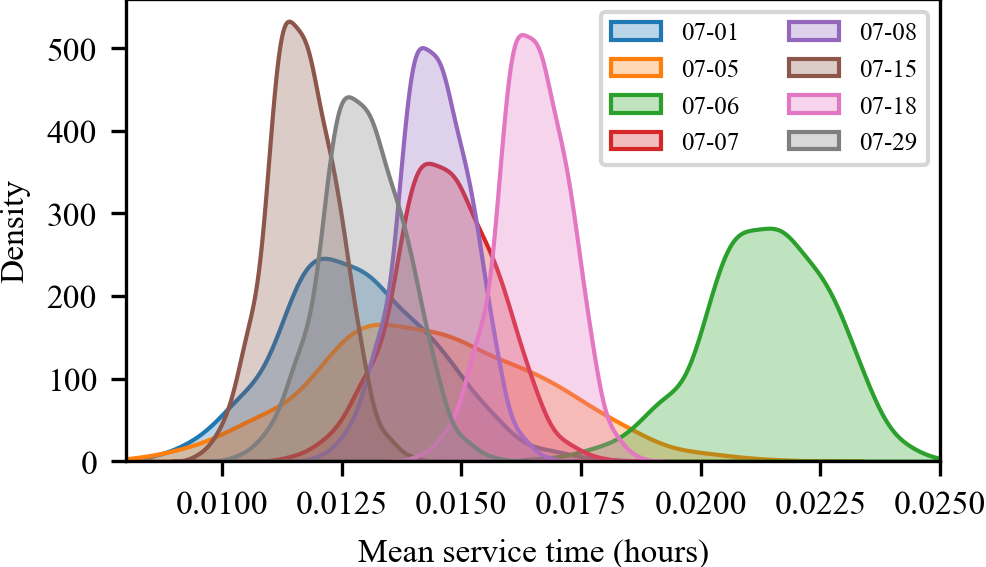
\includegraphics[width=0.8\linewidth]{media/s_phi_2019-07_selection.png}
    \caption{A selection of separate posterior approximations for individual subsamples of the full dataset, each corresponding to a single day from July 2019, as listed in the legend.}
    \label{fig:s-phi-selection}
\end{figure}


\begin{table}[htb]
    \centering
    \begin{tabular}{|c||c|c|}
        \hline
        Date & $\hat\mu$ (hrs) & $\hat\sigma$ (hrs) \\
        \hline\hline 
        2019-07-01 & 0.01283 & 0.002107 \\
        \hline
        2019-07-05 & 0.01427 & 0.002271 \\
        \hline 
        2019-07-06 & 0.02123 & 0.002229 \\
        \hline
        2019-07-07 & 0.01472 & 0.002315 \\
        \hline
        2019-07-08 & 0.01451 & 0.002305 \\
        \hline 
        2019-07-15 & 0.01181 & 0.001953 \\
        \hline
        2019-07-18 & 0.01650 & 0.002414 \\
        \hline
        2019-07-29 & 0.01305 & 0.002140 \\
        \hline
    \end{tabular}
    \caption{Estimated mean $\hat\mu$ and standard deviation $\hat\sigma$ in hours for daily posteriors $\svn$.}
    \label{tab:s-phi-selection}
\end{table}


\subsection{Final Loss Construction}

This breaks up our optimization problem into two steps. First, we wish to find individual
\begin{equation}
    \hat\psi^{(k)}, \hat\theta^{(k)} = \argmax_{\psi,\theta} \underbrace{\EX{\rz\sim\svd{\cdot\given x^{(k)};c^{(k)}, y^{(k)}}}{\log\frac{\pld{x^{(k)}\given z, y^{(k)}}\pld{z;c^{(k)}}}{\svd{z\given x^{(k)};c^{(k)}, y^{(k)}}}}  }_{\elbo{s}{\psi, \theta, x^{(k)}; c^{(k)}, y^{(k)}}}
\end{equation}
for each $(x^{(k)},w^{(k)}, y^{(k)})\in\Data$, where $c^{(k)}=\fvd{w^{(k)}}$. For clarity, we re-iterate that we have specifically learned these variational approximations $\svd{z\given y;c}$ for each $y$ and $c$, and $\svn$ does not immediately accept $y$ as an input. Also, in our case, $\theta$ as pertains to $\pld{x\given z;y}$ is assumed to be empty, so we are really just finding $\hat\psi^{(k)}$. Once we have learned these, we then approximate
\begin{equation}
    \elbo{q}{\phi,\theta,x;c,d,y}\approx \log \pld{x;c,y} - \DKL{\qvd{\cdot ; d}}{\svd{\cdot \given x;c,y}},
\end{equation}

and just use this as usual in our previously derived
\begin{equation}
    \hat\phi,\hat\theta,\hat\nu,\hat\gamma = \argmax_{\phi,\theta,\nu,\gamma} \sum_{(x,y,w)\in \Data} \elbo{q}{\phi,\theta,x;\fvd{w},\gvd{x,y,w},y}.
\end{equation}

\begin{proposition}[Final Loss Construction]
    To fit loss conventions, we negate this and instead solve the mirrored problem
    \begin{equation}
        \hat\phi,\hat\theta,\hat\nu,\hat\gamma = \argmin_{\phi,\theta,\nu,\gamma} \sum_{(x,y,w)\in \Data} -\elbo{q}{\phi,\theta,x;\fvd{w},\gvd{x,y,w},y}.
    \end{equation}    
\end{proposition}



\section{Implementation Details}
\label{sec:atrds-implementation}
For learning the individual posteriors $\svd{z\given x;c,y}$ for each $(x,y,w)\in\Data$ and $c\in \{0,1\}$, we use Pyro's SVI library \cite{bingham2019pyro}, to smoothly integrate with our air traffic simulation which is implemented as a probabilistic model in the same language. We use a multivariate Gaussian distribution as the variational family, automatically transformed to fit a positivity constraint we place on the mean service time $z$ in the probabilistic program.

For learning $\qvd{z;c,d}$, we use a conditional normalizing flow as the variational family. Specifically, we use the neural spline flow architecture \cite{durkan2019neural} with $3$ stacked transforms, and $2$ hidden layers of $16$ units each, using a Rectified Linear Unit (ReLU) activation. The context dimension for conditioning is $5$, where the first four entries represent a one-hot encoding for $d$ through each combination of the $d_x$ and $d_y$ components, and the fifth entry is the $d_w$ component, given by $\gvn$. In other words, we transform the 3-dimensional label $d$ to a 5-dimensional label $\widetilde{d}$, only for training the normalizing flow to encourage further decoupling of the clusters, as show in \cref{tab:d-training-labels}.
% \begin{align}
%     d = (0,0,d_w)&\implies (1,0,0,0,d_w)=\widetilde{d},\\
%     d = (0,1,d_w)&\implies (0,1,0,0,d_w)=\widetilde{d},\\
%     d = (1,0,d_w)&\implies (0,0,1,0,d_w)=\widetilde{d},\\
%     d = (1,1,d_w)&\implies (0,0,0,1,d_w)=\widetilde{d}.
% \end{align}

\begin{table}[htb]
    \centering
    \begin{tabular}{c||c}
        $d$ & $\widetilde{d}$ \\
        \hline\hline
        $(0,0,d_w)$ & $(1,0,0,0,d_w)$ \\
        \hline
        $(0,1,d_w)$ & $(0,1,0,0,d_w)$ \\
        \hline
        $(1,0,d_w)$ & $(0,0,1,0,d_w)$ \\
        \hline
        $(1,1,d_w)$ & $(0,0,0,1,d_w)$ \\
    \end{tabular}
    \caption{Corresponding training label $\widetilde{d}$ for each cluster label $d$.}
    \label{tab:d-training-labels}
\end{table}

We directly implement everything for this part in PyTorch, using the Zuko library for the normalizing flows architecture \cite{rozet2024probabilists}.

For optimization, we use the Adam optimizer with an initial learning rate $5\times 10^{-3}$ and an exponential decay schedule with final learning rate $10^{-3}$. For all SVI parameters, we clip gradient norms at $100$, and all classification parameters at $10$. The $\svn$ training process is run for $500$ iterations, and the $\qvn$ training process is run for $1000$ iterations, where $\phi$ is frozen at step $500$ to allow some time for $\nu$ and $\gamma$ to fully stabilize.

\section{Results and Discussion}
\label{sec:atrds-results}
After learning our separate posteriors and clustering $\gvn$, along with the weather thresholds used in $\fvn$, we can now analyze and apply our results to our original goals of understanding and generating failure conditions.

\subsection{Analyzing Learned Posteriors}

For our two user-defined parameters, we choose $\xth=15$ minutes for our delay threshold and $\yth=72$ operations per hour for our demand threshold in $\gvn$. For both $\fvn$ and $\gvn$, we use $\alpha=50$ as the boundary sharpness scaling parameter. Although LGA is currently supposed to have hourly limits of 71 for scheduled operations and 3 for unscheduled operations during slot-controlled hours, historical practices still allow for scheduled operations to be between 72 and 75 in most hours \cite{faa_lga_2024}. The final results of the learned parameters are
% \begin{align}
%     \wthvf&=1.392,\qquad
%     \wthcf=1318,\qquad\\
%     \wthvg&=1.600,\qquad
%     \wthcg=1276,
% \end{align}
\begin{table}[htb!]
    \centering
    \begin{tabular}{|c||c|c||c|c|}
        \hline
        Parameter & Value & Units & Type & Function\\
        \hline\hline
        $\wthvf$ & $1.392$ & miles & visibility & $\fvn$ \\
        \hline
        $\wthvg$ & $1.600$ & miles & visibility & $\gvn$ \\
        \hline\hline
        $\wthcf$ & $1318$ & feet & ceiling & $\fvn$ \\
        \hline
        $\wthcg$ & $1276$ & feet & ceiling & $\gvn$ \\
        \hline
    \end{tabular}
    \caption{Final learned visibility and ceiling thresholds}
    \label{tab:learned-thresholds}
\end{table}

where $\wthvf$ and $\wthvg$ are in statute miles and $\wthcf$ and $\wthcg$ are in feet. Our final ELBO loss, i.e. negated ELBO, was $-204.34$ nats/dim. \cref{fig:q-phi-combined} shows the posterior distributions for the learned mean service times constructed from $10000$ samples for each cluster determined by $d= \gvd{x,y,w}$, for each of the eight labels $d\in \{0,1\}^3$, and \cref{tab:q-phi-results} displays some summary statistics. We can see that the posteriors appear to be reasonable, because the more nominal posteriors are near $0.0125$ hours, a mean service time which corresponds to a realistic capacity of $80$ operations per hour for LGA.

\begin{figure}[htb!]
    \centering
    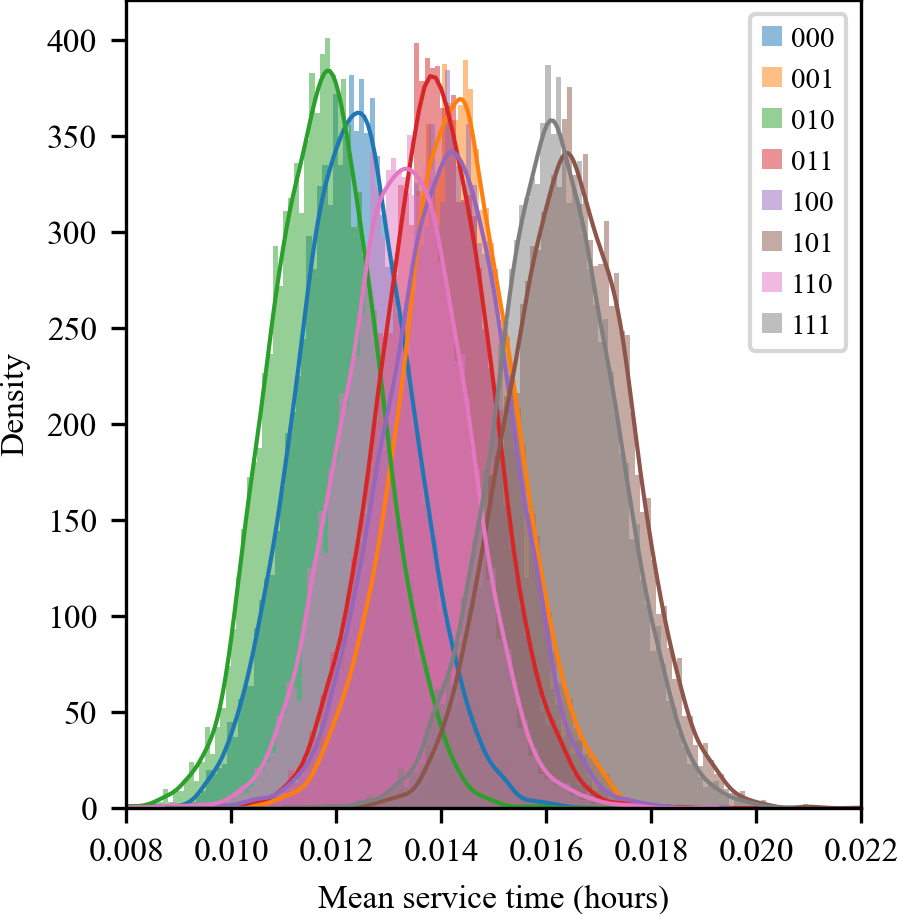
\includegraphics[height=3.0in]{media/q_phi_nsf_730_all.png}
    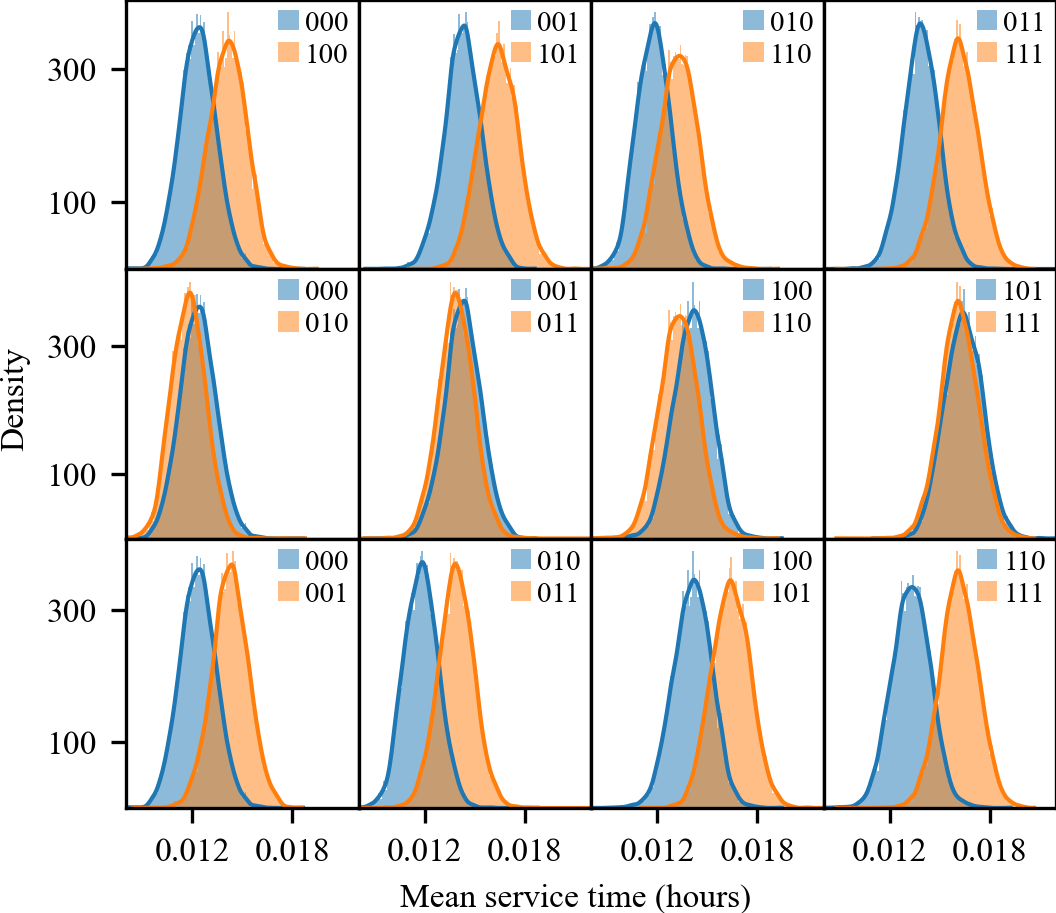
\includegraphics[height=3.0in]{media/q_phi_nsf_730_grid.png}
    \caption{Variational approximations for the mean service time $\rz$, for eight cluster labels $d\in\{0,1\}^3$. On the left, we plot the posteriors for all eight clusters for comparison. On the right, we plot pairs where two components of the label are held constant for each value in $\{0,1\}^2$ across the row, and the third is varied between $\{0,1\}$, with $d_x$, $d_y$, and $d_w$ being varied in the first, second, and third rows, respectively.}
    \label{fig:q-phi-combined}
\end{figure}

% 000 posterior, mean=0.01234, std=0.00110
% 001 posterior, mean=0.01429, std=0.00111
% 010 posterior, mean=0.01178, std=0.00104
% 011 posterior, mean=0.01389, std=0.00109
% 100 posterior, mean=0.01411, std=0.00116
% 101 posterior, mean=0.01643, std=0.00116
% 110 posterior, mean=0.01329, std=0.00117
% 111 posterior, mean=0.01617, std=0.00115

\begin{table}[htb]
    \centering
    \begin{tabular}{|c|c|c||c|c|}
        \hline
        $d_x$ & $d_y$ & $d_w$ & $\hat\mu$ (hrs) & $\hat\sigma$ (hrs) \\
        \hline\hline
        0 & 0 & 0 & 0.01234 & 0.00110 \\
        \hline
        0 & 0 & 1 & 0.01429 & 0.00111 \\
        \hline
        0 & 1 & 0 & 0.01178 & 0.00104 \\
        \hline
        0 & 1 & 1 & 0.01389 & 0.00109 \\
        \hline
        1 & 0 & 0 & 0.01411 & 0.00116 \\
        \hline
        1 & 0 & 1 & 0.01643 & 0.00116 \\
        \hline
        1 & 1 & 0 & 0.01329 & 0.00117 \\
        \hline
        1 & 1 & 1 & 0.01617 & 0.00115 \\
        \hline
    \end{tabular}
    \caption{Estimated mean $\hat\mu$ and standard deviation $\hat\sigma$ in hours for learned posteriors $\qvn$.}
    \label{tab:q-phi-results}
\end{table}

Using the pairwise comparison plots in the grid on the right side of \cref{fig:q-phi-combined}, we can investigate the effect of each component of $d$ on the learned posterior for its cluster. In the first row, where only $d_x$ is varied in each plot, we note that the posteriors for $d_x=0$ (blue) are to the left of those for $d_x=1$ (orange). This shows that introducing more delays corresponds to shifting the learned posterior to the right, which is what we expected to see. Similarly, in the third row, where only $d_w$ is varied in each plot, we note that the posteriors for $d_w=0$ (blue) are to the left of those for $d_w=1$ (orange), which also aligns with the belief that worse weather leads to higher service times that we incorporated into the model.

In the second row, where only $d_y$ is varied in each plot, we observe a slightly different effect, although it is a bit less evident. Here, the posteriors for $d_y=0$ (blue) appear to be shifted to the right, in comparison to $d_y=1$ (orange). However, this still makes sense, because it is showing the effect of scheduled demand on delay that we had previously discovered in \cref{sec:atrds-single-airport}, that because of the higher scheduled demand, a lower mean service time may be required to achieve the same performance in terms of delays on a busier day versus a lighter one, all else held equal, which manifests here as the posterior for that particular cluster being shifted to the left slightly.


\subsection{Using Learned Posteriors}

Now that we have learned posteriors for our separate clusters, we can use them in our learned generative model, and analyze the results, similar to sampling from the posterior predictive distribution after learning an approximation for the posterior. 

\begin{figure}[htb!]
    \centering
    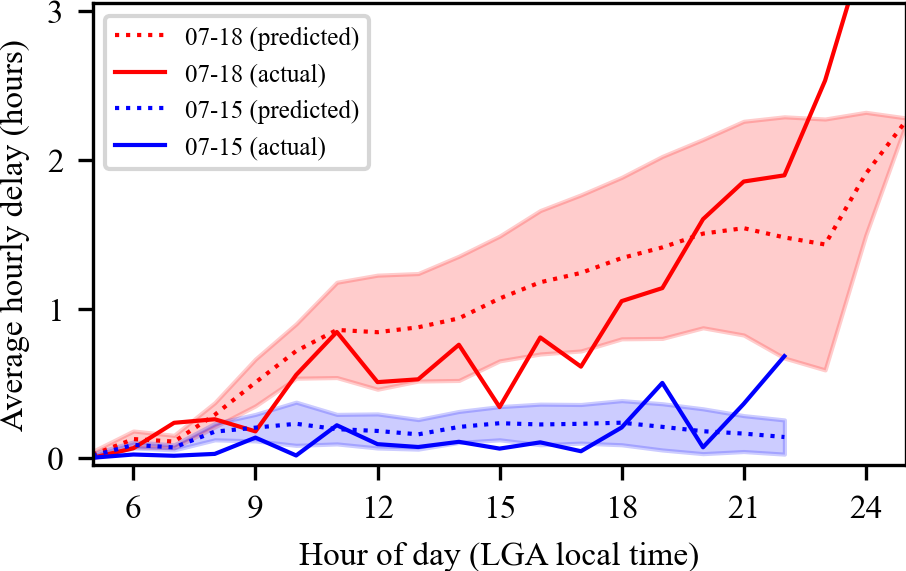
\includegraphics[width=0.7\linewidth]{media/posterior_predictive_comparison.png}
    \caption{Actual and predicted mean hourly delays using our model, with a weather-induced delay applied on one day (red) and nominal operations on the other (blue).}
    \label{fig:pp-comparison}
\end{figure}

We first select two days for analysis, which are July 18, 2019 (day 1) and July 15, 2019 (day 2). For both days, the peak scheduled hourly demand is $75$ operations, which is above $\yth$, so $d_{y,1}=d_{y,2}=1$. Additionally, the weather values for each day are $w_1=(10.0, 8649.3)$ and $w_2=(2.414,299.2)$, so $d_{w,1}\approx 0$ and $d_{w,2}\approx 1$. In reality, day 1 (red) has high delays above $\xth$, while day 2 (blue) does not, as seen in the solid lines in \cref{fig:pp-comparison}, so for comparison, we also select $d_{x,1}=1$ and $d_{x,2}=0$. Then, using each of these posteriors corresponding to $d_1$ and $d_2$ in the model, we can generate predictive samples, shown in the dotted lines and shaded regions in the figure. These are consistent with the actual outcomes, which shows that our learned generative model is able to accurately take in conditions of interest and generate a realistic result of imposing them onto a given day, showing its value as a predictive tool. The key here is that we can take $y$ and $w$ for a new day, which we would know from a schedule and forecast, respectively, and come up with distributions for $z$ that should lead to a desired level of delay, and doing so does appear to match what actually happens.

\begin{figure}[htb!]
    \centering
    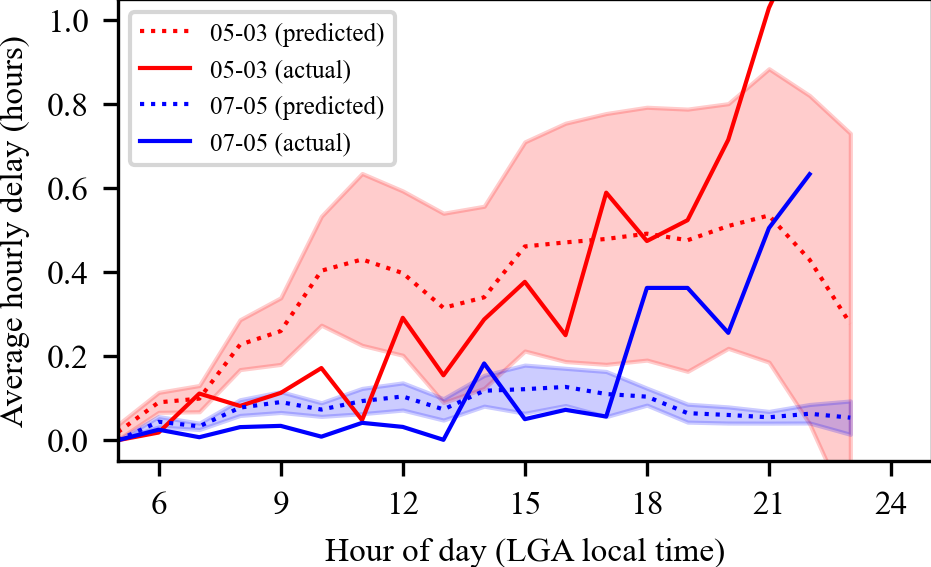
\includegraphics[width=0.7\linewidth]{media/posterior_predictive_comparison_alt.png}
    \caption{Actual and predicted mean hourly delays using our model, with a demand-induced delay applied on one day (red) and nominal operations on the other (blue).}
    \label{fig:pp-comparison-alt}
\end{figure}

% Actual vs predicted hourly delay using our model for two days, the plot in red shown for a day with weather-induced delay that our model successfully replicates (predicted average and standard deviation for 20 samples shown in the plots). The plot in blue shows hourly delays for a day with observed delays to be less than 15 minutes.

Similarly, we examine another pair of days, May 3, 2019 (day 1) and July 5, 2019 (day 2). This time, we have $w_1=(1.609,162.7)$ and $w_2=(10.0,574.9)$, so $d_{w,1}\approx d_{w,2}\approx 1$. However, this time we have $y_1$ above the threshold $\yth$ and $y_2$ below it, so $d_{y,1}=1$ and $d_{y,1}=0$. Similarly to before, we follow the actual observation for comparison, so we use $d_{x,1}=1$ and $d_{x,2}=0$. We visualize this in \cref{fig:pp-comparison-alt}, where we can see the effect of varying the imposed demand in our generative model, and that it also resembles reality for the two day in question.

In these two case studies, we have seen that our learned model and posteriors, although somewhat coarse, do appear to be capable of generating useful and realistic results. Because of the simplified model, we can simply sample adversarial weather conditions by using the learned thresholds, but we will leave investigating more complex structures as part of the plan for future work.

\section{Summary}
\label{sec:atrds-summary}

In this chapter, we developed a guiding case study on weather and delays at LGA. First, we analyzed weather and schedule data along with observed delays to motivate both the choice of weather variables and inclusion of both weather and schedule data, as opposed to just weather data. Then, we developed an amortized variational inference based framework for simultaneously clustering data points into meaningful groups and learning representatives posteriors for each group, and showed via implementation that our learned generative model can produce useful predictive results.
\chapter{Conclusion}
\label{ch:conclusion}

% This proof of concept was developed mainly in January 2025 for a manuscript to be submitted to the US-Europe Air Transportation Research \& Development Symposium (ATRDS).

In \cref{ch:atrds}, we examined a simplified problem formulation to understand how we would begin to go about bridging the gap between purely data-driven analysis and existing domain knowledge. To go beyond this guiding example, there are at least a few natural directions for further extension and study.

The first is to go further in what we are hoping to understanding from an air traffic management perspective. In particular, we note that we have not yet considered in depth how air traffic managers are meant to interact with the simulation or any other part of the overall process, and so \cref{app:atm} will focus on bridging that gap. A second idea is gaining a better understanding of how exactly we can quantify risk, especially in a more complex network scenario where it is less immediately obvious how to construct a single exceedance probability, which we will discuss further in \cref{app:risk}. This will enable more flexibility in how we interact with the notion of risk and failure in our data-driven approach. Third, in \cref{app:shrinkage}, we will continue along the previously introduced concept of robustly combining information when the quantity or quality of data is less than ideal. 

It is important to stress a couple points here, most importantly, that these directions are far from comprehensive. As even the problem itself is not particularly well-defined without some work, there are many possible directions to further investigate, some of which we will note in this chapter as well.


\section{Future Work}

\subsection{Extending the Guiding Case Study} For our guiding case study specifically, we plan to extend the method from a single airport study to a larger network, so that we can capture a wider range of latent parameters than just a single mean service time. We also note that we run into some limitations because of the simplifying choices made. For example, choosing simple threshold-based structures for $\fvn$ and $\gvn$ may not work as well when working with more complex problems, and we plan to investigate more general mixtures, in a similar idea to what is studied in \cite{flowgmm2019}. Along similar lines, introducing more direct support for actions, similarly to what is implemented for a different non-stochastic simulator in \cite{michael_peng_probing_2024}, is another direction for future study. Finally, we could attempt to relax the requirement of having access to both likelihoods and gradients from the simulator, and also introduce explicit methods for working with more limited data, by considering other methods such as \cite{parashar2024failure, maurya2016, dawson2024breaking}.

\subsection{Learning Surrogate Models}

For completeness, we will also consider dropping the assumption that we already know some part of underlying structure of the true data distribution (e.g. through simulation), and working the problem of working directly with the available data. In other words, this would be only looking at the case of $\rw\leftrightarrow \rx$. Here, our goal is to learn some structure for our paired observations in an unsupervised manner. For example, the originally considered idea of directly using a diffusion model to generate novel weather examples that correspond to failure flight days would fall under this category. On its own, this can serve as a baseline to compare results against, though it may be difficult to learn anything useful if we do not have enough data. Additionally, the results would be less interpretable than an approach that specifies more of the underlying model, since we do not necessarily learn a latent space that represents anything meaningful. However, learning such a surrogate model may still be useful as a component of other approaches for failure modeling and prediction.

\subsection{Actively Generating Failures} 

Here, we will assume that we are working with a $\rw\to \rz\to \rx$ hierarchical model, where, in the language of the air traffic problem, $\rx$ are the observed delays, $\rz$ are simulation parameters such as mean service and turnaround times at individual airports, and $\rw$ are weather conditions. The problem of generating failure conditions can be framed as finding values of $w$ or $z$ such that $\PP(x\in \Omega_f\given w)>\pi_f$ or $\PP(x\in\Omega_f\given z)>\pi_f$, respectively, where $\Omega_f$ is some set of values $x$ that we consider failures (e.g. delays above fifteen minutes), and $\pi_f\in [0,1]$ is some threshold for failure risk. In other words, we want to find values $w$ or $z$ such that $x$ is likely to fall in $\Omega$.

The problem of finding values of $z$ only, which, because of the conditional independencies, restricts us to the $\rz \to \rx$ part of the model, is well-studied, so in our case this may be just applying existing methods to find failure inputs for whatever air traffic simulator we are interested in. When introducing $w$, the problem is a bit more complicated if we also need to learn $\rw\to\rz$. Since this part is often more difficult to model satisfactorily, learning a black-box surrogate model for it may be preferable, but does sacrifice some interpretability of results.

Now comes the ``active'' part. What happens if the the simulation is allowed to change after each new failure we discover? Naturally, training and planning on the part of air traffic managers is a plausible scenario in which we could enact a failure discovery and repair loop. For example, we could consider a simulation in which the traffic managers are able to use their current knowledge to control some parts of it, such as by imposing traffic management initiatives. Then, in the current iteration, we might attempt to generate adversarial conditions that they have trouble dealing with. However, if these difficult conditions are reduced to normal conditions because of planning around the observed failure mode to mitigate future incidents, our strategy for generating failure conditions would likely have to adjust in the next iteration as well. This sort of alternating adversarial optimization formulation is one we have not yet considered, but it is one that is both interesting and practically relevant. Some related work in the failure prediction and repair cycle, from a slightly different perspective, can be found in \cite{dawson2024breaking, 10925872, DBLP:journals/corr/abs-2203-02038}.


%%% Appendicies of thesis  %%%%%%%%%%%%%%%%%%%%%%%%%%%%%%%%%%%%%%%%%%%%%%%%%%%%%%%%%%%%%%%%%%%%%%%%

\appendix

\chapter{Appendix to Chapter~\ref{ch:atrds}}
\label{app:atrds}

Code for the \href{https://github.com/jz268/atm_generative}{data} and \href{http://github.com/jz268/BayesAirATRDS2025}{inference} components provided on github at their respective links.

\section{Gradient Boosted Tree Regression}

As an initial step before we developed the method in \cref{ch:atrds}, we first attempted to reproduce the results of previous studies that used gradient boosted trees to directly regress on flight data from individual flights, with associated meteorological conditions at the corresponding time \cite{WU2022100030} One finding was that departure delay was a significant factor, which makes sense because if a flight leaves its origin late, it will also arrive at its destination late unless it tries to make up some time along its route, which may not always be possible.

After cleaning, processing, and merging the schedule and weather data for flights between Los Angeles International Airport (LAX) and John F. Kennedy International Airport (JFK), we found similar results using the XGBoost library \cite{Chen:2016:XST:2939672.2939785}. \cref{fig:importance-arr-dep} shows feature importance, based on the default ``number of times a feature is used to split the data across all trees'', when the target variable is set to either arrival or departure delay. Here, ``DepTimeMinutes'' refers to departure time, and ``CRSDepTimeMinutes'' refers to scheduled departure time. Both times are in minutes past midnight. As expected, we see that the most significant feature is departure time in both cases.

\begin{figure}
    \centering
    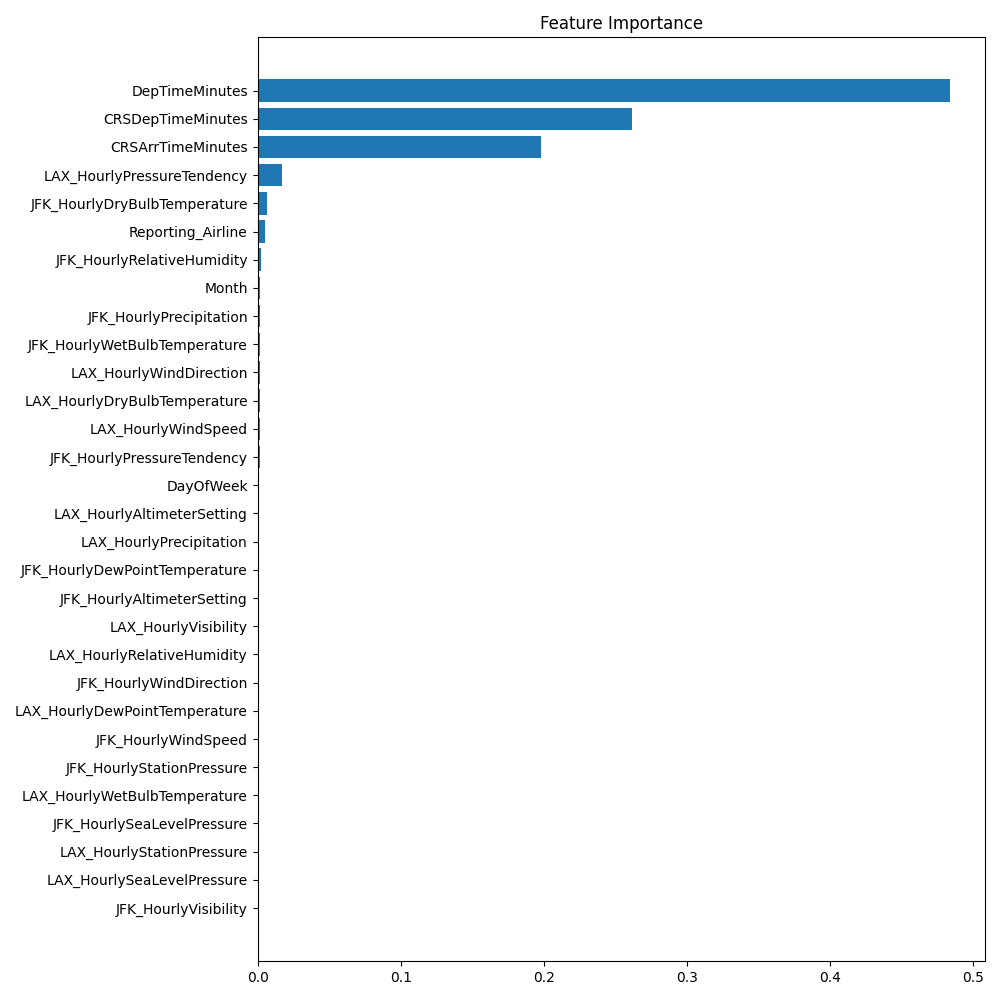
\includegraphics[width=0.49\linewidth]{media/features_ArrDelay.png}
    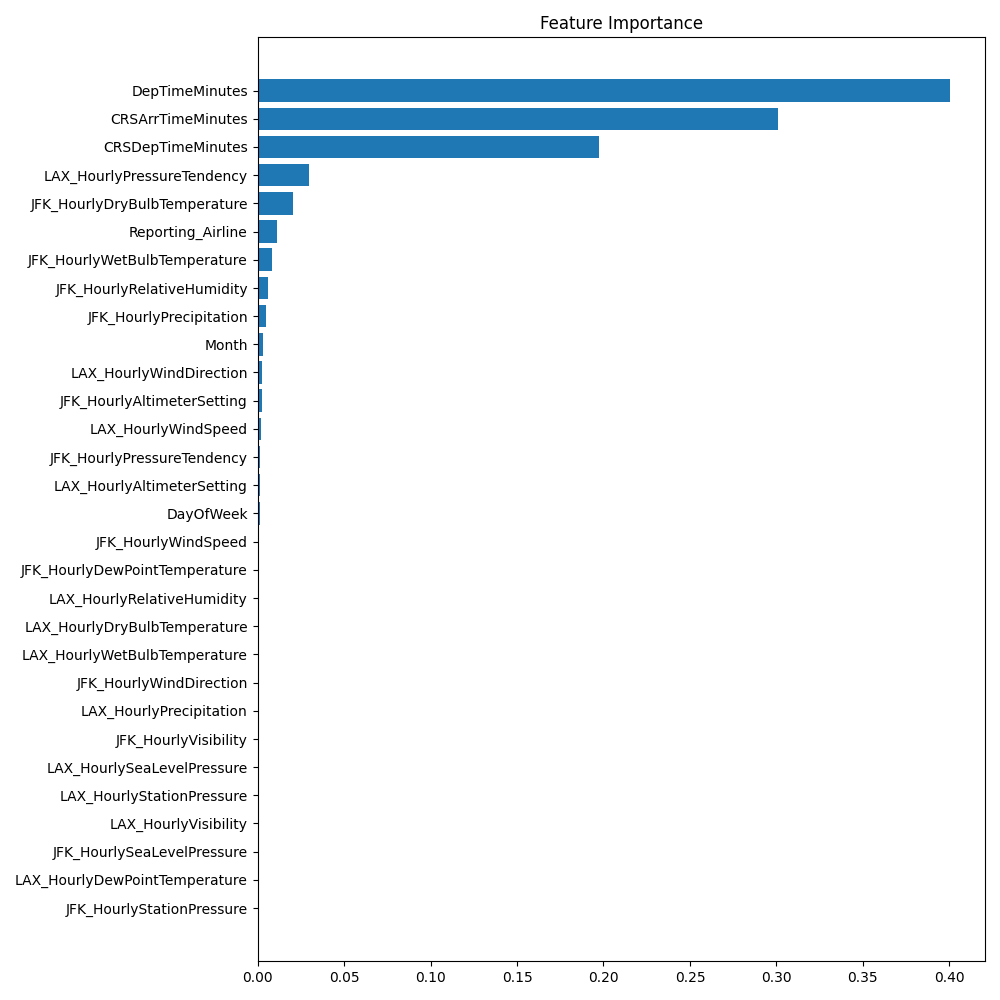
\includegraphics[width=0.49\linewidth]{media/features_DepDelay.png}
    \caption{Feature importance when target is arrival (left) and departure (right) delays.}
    \label{fig:importance-arr-dep}
\end{figure}

\begin{figure}
    \centering
    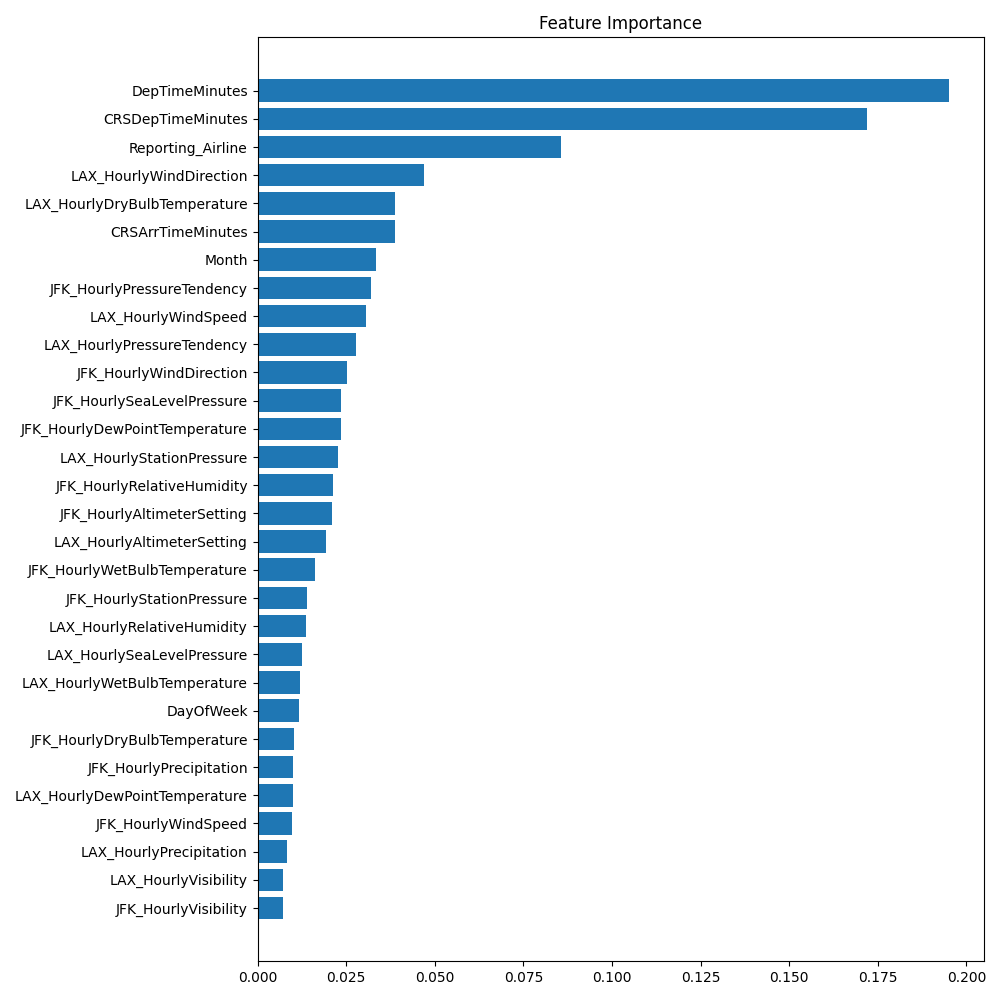
\includegraphics[width=0.49\linewidth]{media/features_NASDelay.png}
    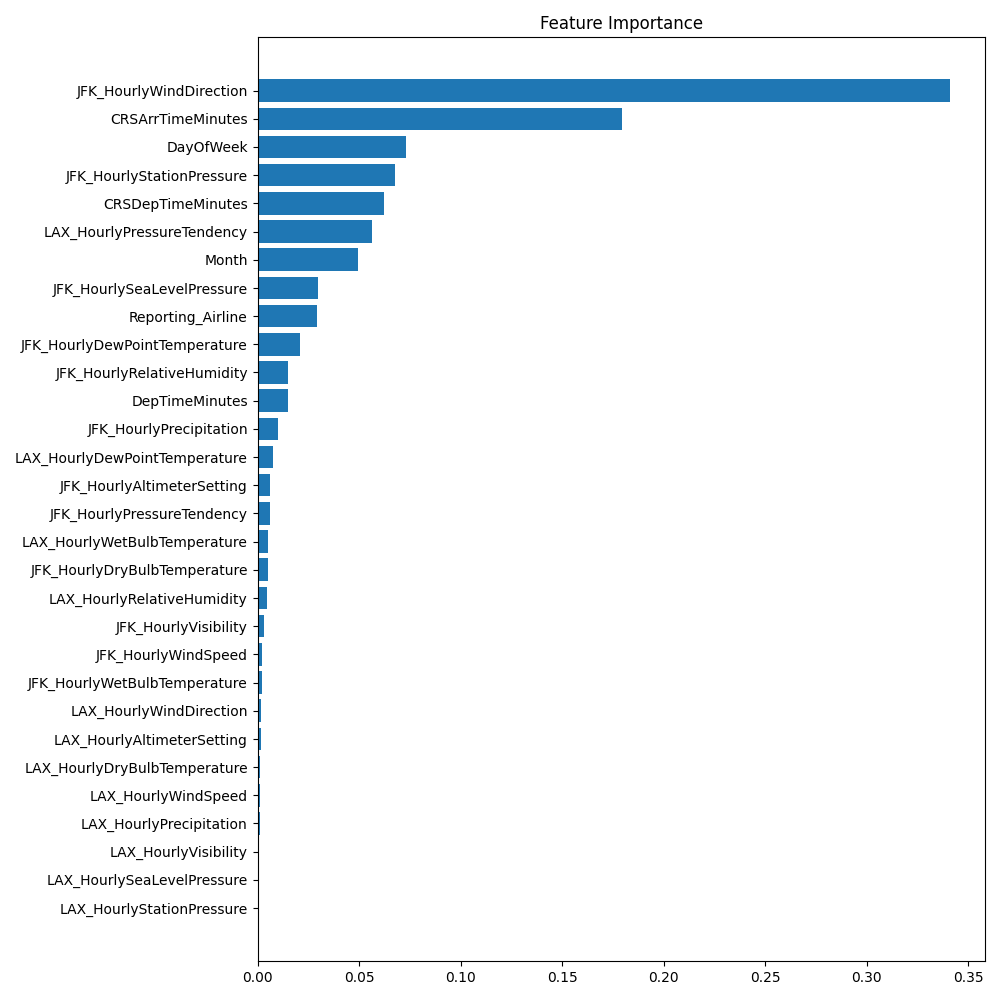
\includegraphics[width=0.49\linewidth]{media/features_WeatherDelay.png}
    \caption{Feature importance when target is NAS (left) and weather (right) delays.}
    \label{fig:importance-nas-weather}
\end{figure}

For NAS and weather delays in \cref{fig:importance-nas-weather}, we also see similar results, but they are slightly different. This is probably because there was not actually that much data with an NAS delay or weather delay actually reported, in comparison to the usual arrival and departure delays. We also tried to isolate the accumulated delay at a particular airport, which we called ``NewDelay'', from subtracting the departure delay from the arrival delay of a flight. Feature importance is shown in \cref{fig:importance-new}. We can see that we do not have any useful results anymore. This suggests that working with flights individually is not enough, and that we need to include the temporal structure somehow, for example, by working with entire days at a time similarly to the LGA case study.

\begin{figure}[hb]
    \centering
    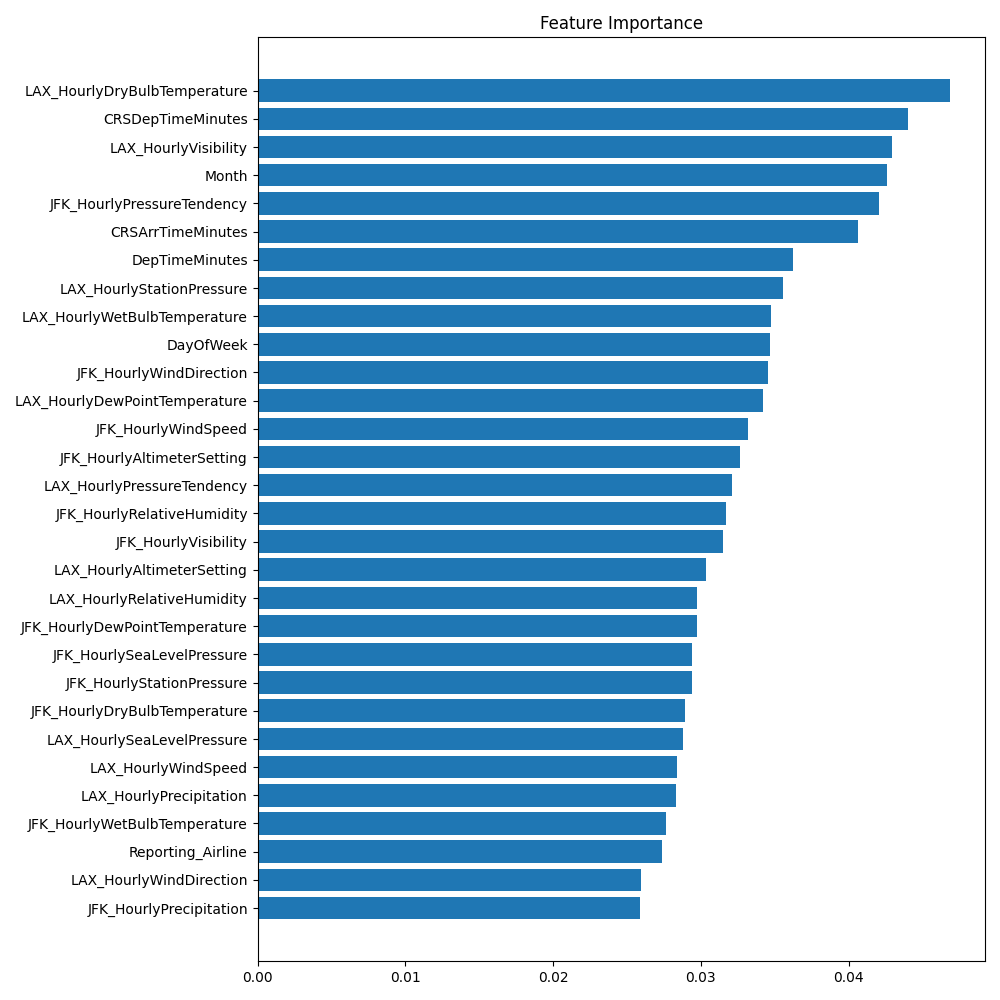
\includegraphics[width=0.75\linewidth]{media/features_NewDelay.png}
    \caption{Feature importance when target is new delays, i.e. arrival minus departure.}
    \label{fig:importance-new}
\end{figure}

\section{Aircraft Flows at LGA}

\begin{figure}[ht]
    \centering
    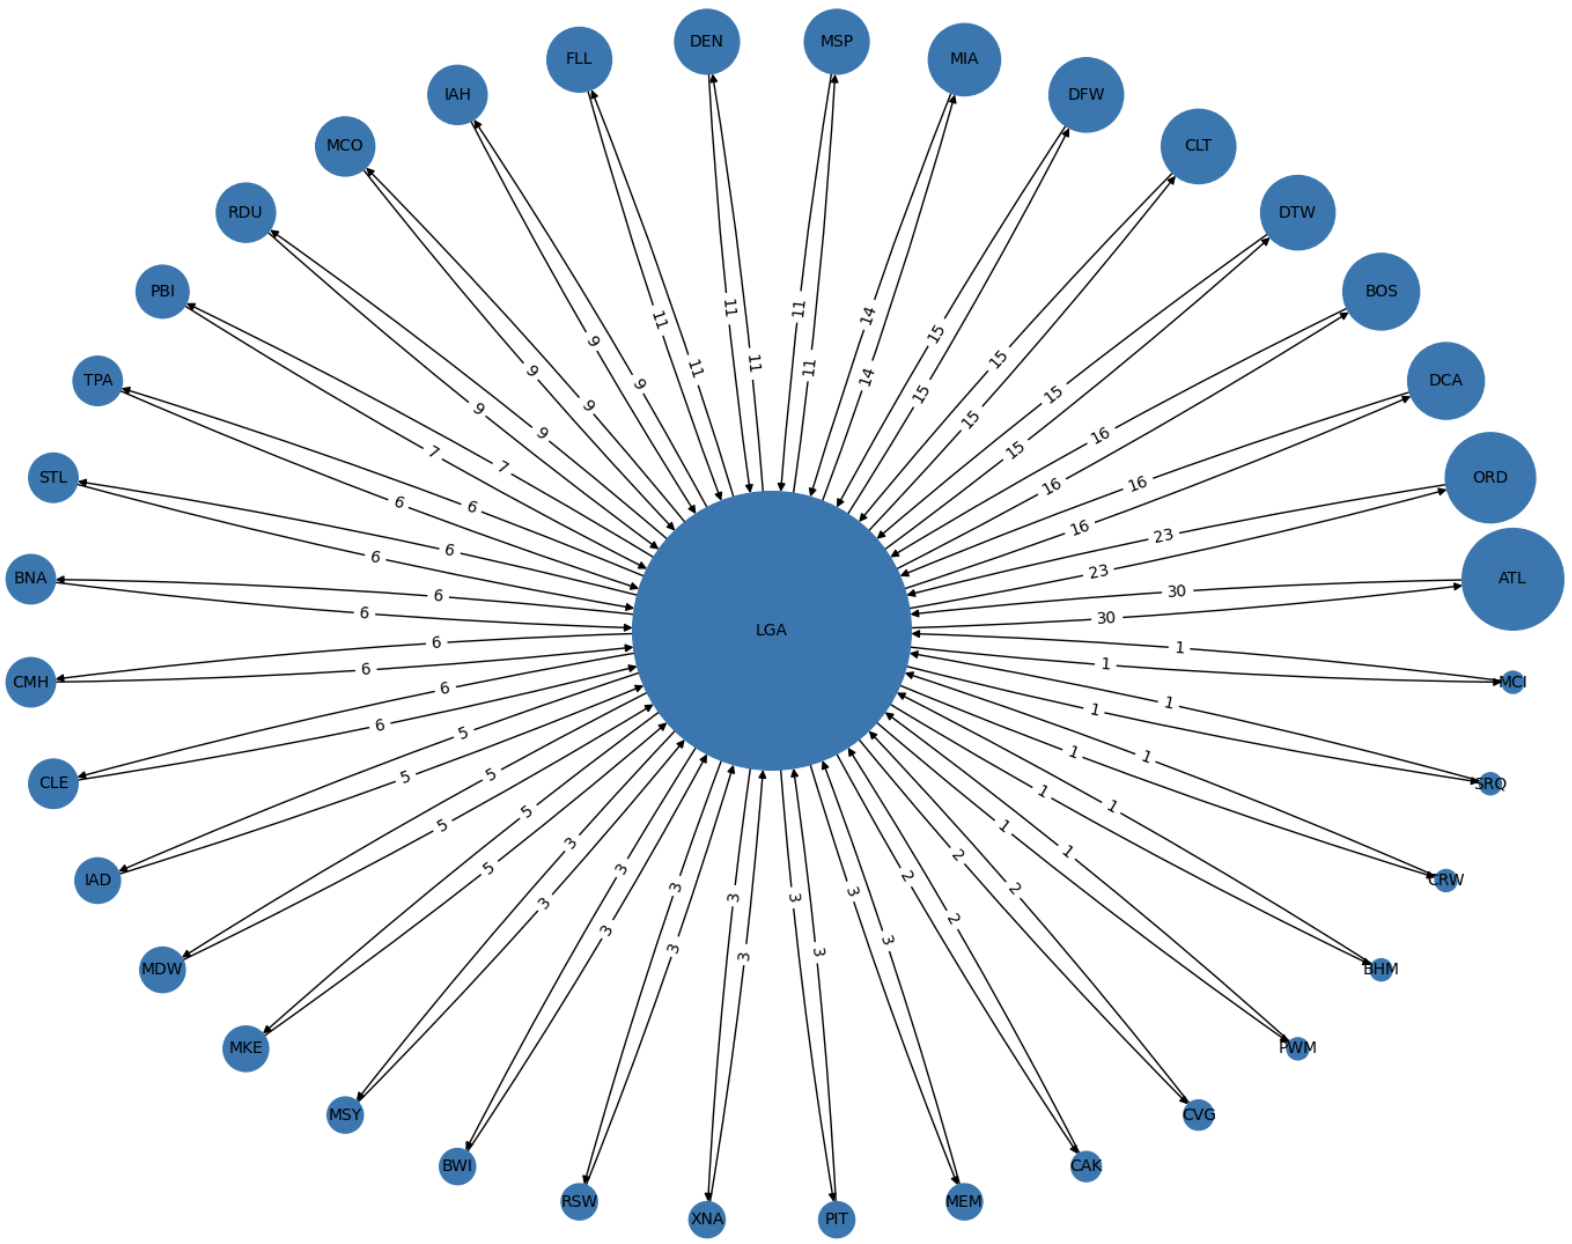
\includegraphics[width=\linewidth]{media/lga_reduced_2012_12_12_clean_cropped.png}
    \caption{Counts of both incoming and outgoing flights between LaGuardia Airport and each of its neighbors on 2012-12-12. Larger node size also indicates more flights.}
    \label{fig:lga-flows-diagram}
\end{figure}

\cref{fig:lga-flows-diagram} shows an example day of flights for LGA, represented as a directed network where the weight placed on each edge is the number of flights going in that direction. We can see that flights are scheduled to have the same number going each way, which makes sense because it is desirable for stability to have fleet levels and reserves at a particular node to stay relatively constant over time.

\section{Cascading Cancellations}

One possible direction for improving the simulation would be to more carefully track the likely dependency structure of flights throughout the day, using the schedule. This came up when analyzing days with many cancellations. For some routes, it seemed like the same aircraft was supposed to be used in sequence, but at some point, one flight was canceled, or delayed for a long time due to diversion, and all subsequent flights were then canceled. With a single airport, it is not as complicated, especially since many flights seemed to mainly be going back and forth between two nodes. However, the network case is likely more complicated, especially since different airlines may schedule their fleet differently.

\chapter{Air Traffic Management}
\label{app:atm}

Earlier, in \cref{ch:atrds}, we did not focus as much on the particulars of the air traffic management problem specifically, as we were limited to a single airport case. However, when moving to the full network scenario, which has a lot more moving parts, we will need to take a closer look in order to develop a better understanding of how the different parts of the system come together, which will be of use when discussing further simulation building and modeling goals. Furthermore, we will also attempt to cover disruptions to air traffic networks in greater detail, to provide some preliminary background for modeling more complex effects. 

\section{National Airspace System}
\label{sec:atm-nas}

Let us briefly review the components and workings of the National Airspace System (NAS) at a high level view, before we go further in depth into the specific aspects of it that we are focused on. Specifically, we will base our study on information from the following FAA sources and defer to them for a more detailed and specific development: \cite{faa_nas_2023} for a more detailed coverage of flight rules and airspace classifications, as well as \cite{faa_tmi_2024} and \cite{faa_tfm_prez_2009} for more information on air traffic management. The NAS broadly refers to the network built from airspace relevant to domestic air travel, and includes various systems such as airports and landing areas, air navigation facilities, and procedures and regulations. These systems are responsible for maintaining safe and efficient operation of thousands of aircraft concurrently traveling through both controlled and uncontrolled airspace, with many different origins and destinations. We will be mainly focused on air traffic control (ATC) and air traffic management (ATM), which are closely interrelated.

\subsection{NAS Traffic Control}

The airspace over the United States is divided into sectors, also known as Flight Information Regions (FIRs), each managed by an Air Route Traffic Control Center (ARTCC), also sometimes referred to as area control centers. These manage flights as they travel through these sectors, perhaps en-route between an origin and destination, but do not manage airspace around these endpoints. Those smaller regions of airspace surrounding airports and landing areas, also known as Terminal Radar Approach CONtrol (TRACON) airspaces, can also be further subdivided into neighborhoods of airspace surrounding single airports \cite{faa_tfm_overview_2025}.

At each airport, there is an Air Traffic Control Tower (ATCT), which manages takeoffs and landing, as well as ground operations such as taxiing. Going up one level to see what happens in each TRACON region, the supervising facility will similarly be responsible for flights that leave and enter, but will leave operations specific to an airport to their ATCT. Analogously, ARTCCs will manage traffic within their sector, but leave the TRACON specific operations to the relevant facility. Finally, there is also an Air Traffic Control System Command Center (ATCSCC), which oversees all air traffic at a high level, but may leave implementation of certain details to ARTCCs, TRACONs, and ATCTs \cite{faa_tfm_overview_2025}.

For our purposes, we are most interested in the role of the ATCSCC, but it is still important to note this hierarchical structure in managing airspace, as it is directly relevant to the sort of disruptions and responses we will be examining. A basic assumption that we will use liberally is that live tracking information the location of an aircraft at any point is readily available for use at all levels. In practice, this is done using transponders located abroad every aircraft, along with ground and surface radar used at the control facilities. \cite{faa_tfm_prez_2009}

% \jztodo{overview figure. also citations?}

\subsection{Simulation Considerations}

One final point the importance of available simulations, as the NAS itself is obviously not a system that we can or should readily run experiments on. As such, the field of developing high-fidelity simulations that can be applied in real world scenarios to assist traffic management planning and other operational initiatives is one under constant development. 

Simulations are often used by the FAA at both the network level, modeling the entire NAS \cite{faa_sim_2024}, and at the individual airport level, to model the operations of a single airport \cite{faa_lga_2024}. One recent development is the NAS Digital Twin, a flexible simulation environment for airspace operations for both historical and live airspace traffic intended for use in further research into NAS operations \cite{Lauderdale_Windhorst_Coppenbarger_Thipphavong_Erzberger_2024}. These simulations also allow for evaluating the factors of interest such as airspace sector capacities and weather information, by providing them as possible inputs. We will not be focusing too much on the details of constructing these simulations, as it is beyond the scope of our work. However, we will spend some time discussing how to identify key predictors for motivating future modeling and simulation development. 

This is particularly relevant because so far, there are still untapped avenues that have not been covered by the simulations we just introduced. One is that there are multiple stakeholders involved in the full air transportation process, such as the airlines themselves, in addition to just the FAA. Therefore, there may be interest in work specifically from their perspective, for instance, to help improve internal flight and crew scheduling processes for airlines, such as the agent-based model introduced in \cite{michael_peng_probing_2024} to analyze the December 2022 Southwest Airlines scheduling crisis. 

Another consideration is that most simulations so far, both deterministic and stochastic, mainly focus on constructing a model that is only concerned with generating output data, given some set of input parameters. Only recently has more focus been given to models with further abilities such as differentiability, which can be used to accelerate research based on them through gradient-based methods \cite{dawson2024breaking}. Another useful ability is inherently incorporating randomness by way of probabilistic programming, which can be used to obtain analyses and inferences that would not be as feasible with stochastic simulations using simple Monte Carlo methods only \cite{dawson2025rare}. In this sense, we reiterate the distinction between models that are ``black-box'', and models where we have direct access to additional information such as gradients or likelihoods. There is a trade-off in that this additional information often means that a simulation that both meets these goals and is efficient can be difficult to design and construct, as we often must work around certain limitations to maintain these abilities, as we saw in \cref{ch:atrds}. Thus, it is still useful to discuss what sorts of simulated effects are most amenable to going beyond black-box modeling, and what compromises may have to be made in terms of simulation fidelity.

\section{Taxonomy of Disruptions and Responses}
\label{sec:atm-taxonomy}

So far, we have mainly been discussing air traffic control, particularly in the actors responsible for the control of aircraft in different situations and sectors of airspace. Now, we will move to the overall network level, and work more loosely with processing aggregate flight demand and flows in the system as a whole. In doing so, we will begin to see a natural taxonomy of disruptions to the system and their associated responses, which can be used to motivate further work in simulation and analysis. While the framework presented in \cite{enea_analysis_2024} is closely related, we are more interested in considering the problem from an abstract simulation and parameters perspective, so we will not focus as much on the specific factors, such as weather, but rather what we will do with them. Additionally, in our taxonomy, we will place greater emphasis on evaluating disruptions from the perspective of other stakeholders, such as airlines, in addition to just the traffic management point of view.

\subsection{Weather Effects}

As we have already seen several times before, weather is a significant cause behind air traffic operations. Earlier in \cref{ch:atrds}, we examined the specific visibility and ceiling sky conditions, and their effects on the operations at a single airport. Some weather effects naturally cannot be effectively analyzed in such a localized manner, and are inherently more at the network level. For example, convective weather that affects a region of airspace cannot necessarily be tied to a single node in the network, as shown in the \cref{fig:nexrad-example} from \cite{iem_nexrad_mosaic}.

\begin{figure}[htb!]
    \centering
    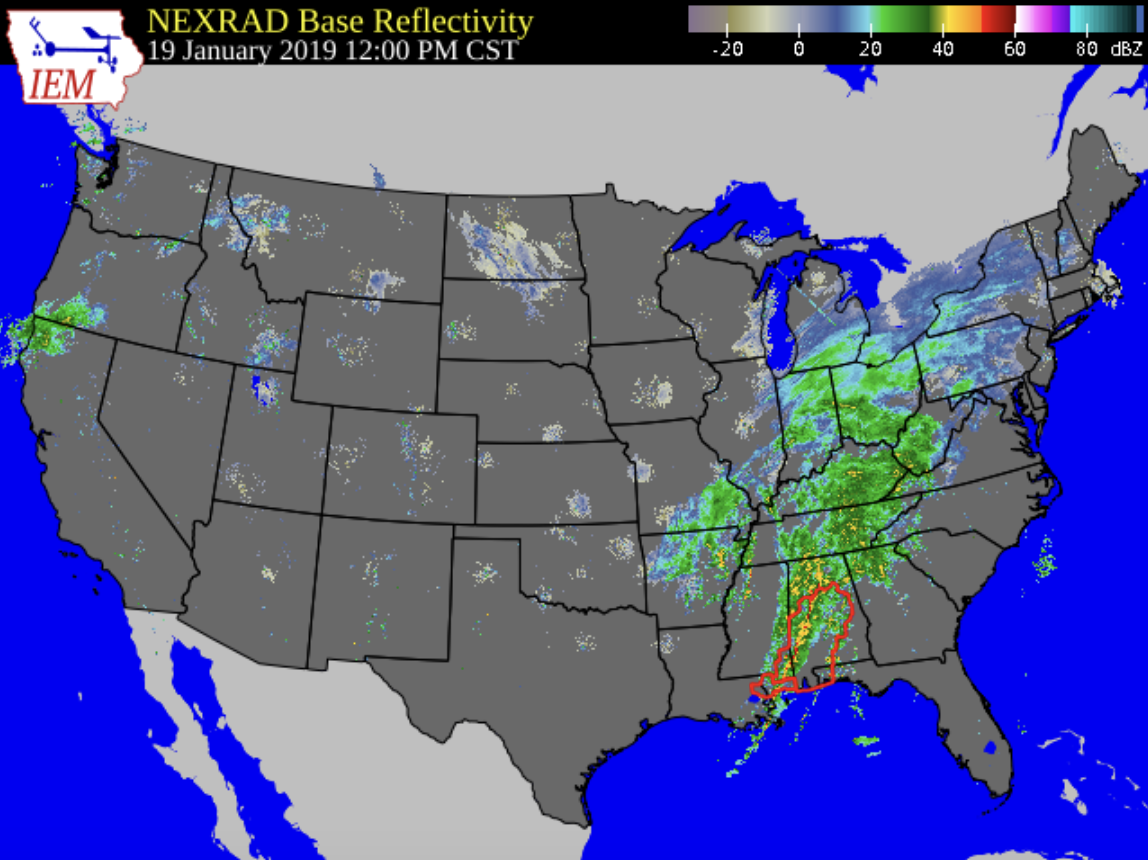
\includegraphics[width=0.49\linewidth]{media/nexrad_2019_01_19_12pm.png}
    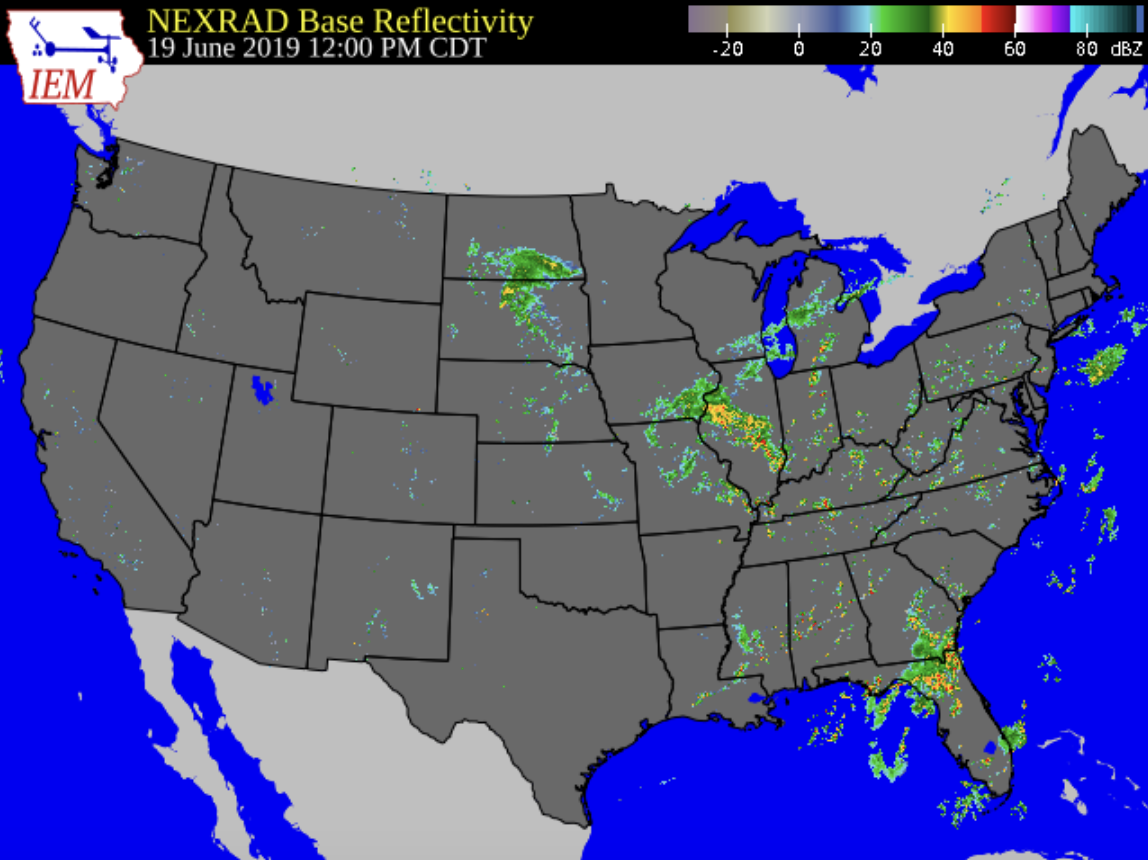
\includegraphics[width=0.49\linewidth]{media/nexrad_2019_06_19_12pm.png}
    \caption{Radar reflectivity maps showing different severities of convective weather from two example days in 2019. The left side shows a more cohesive and globalized convective weather disruption, while the right side shows more sparse and localized disruptions.}
    \label{fig:nexrad-example}
\end{figure}

However, depending on the severity, it may still be possible to consider it localized to a particular sub-network, and consider its aggregated interactions with the rest of the network. Of course, it's often not so simple to just reduce the severity of an event to a single quantity, so we will discuss more about what exactly severity should mean later along with ways to express it in an interpretable manner. Another related factor that can be considered is the frequency of the event, as the processes for handling an area with poor visibility conditions all year round should be very different from planning for much rarer large-scale catastrophic storms.

One point to note is that a localized weather impact can still have network level effects, because of the responses that might be put into place. For example, if a particular node in the network, i.e. a single airport, is under poor weather conditions that make it difficult to service the originally scheduled flow of incoming flights, traffic management initiatives (TMIs) may be implemented to regulate air traffic at a network level. As shown in \cref{fig:gdp-example} from \cite{faa_status_2025}, this is known as a Ground Delay Program (GDP), and shows how issues at a single node of the overall traffic network can easily be broadcast to its neighbors and the rest of the network.

\begin{figure}[htb!]
    \centering
    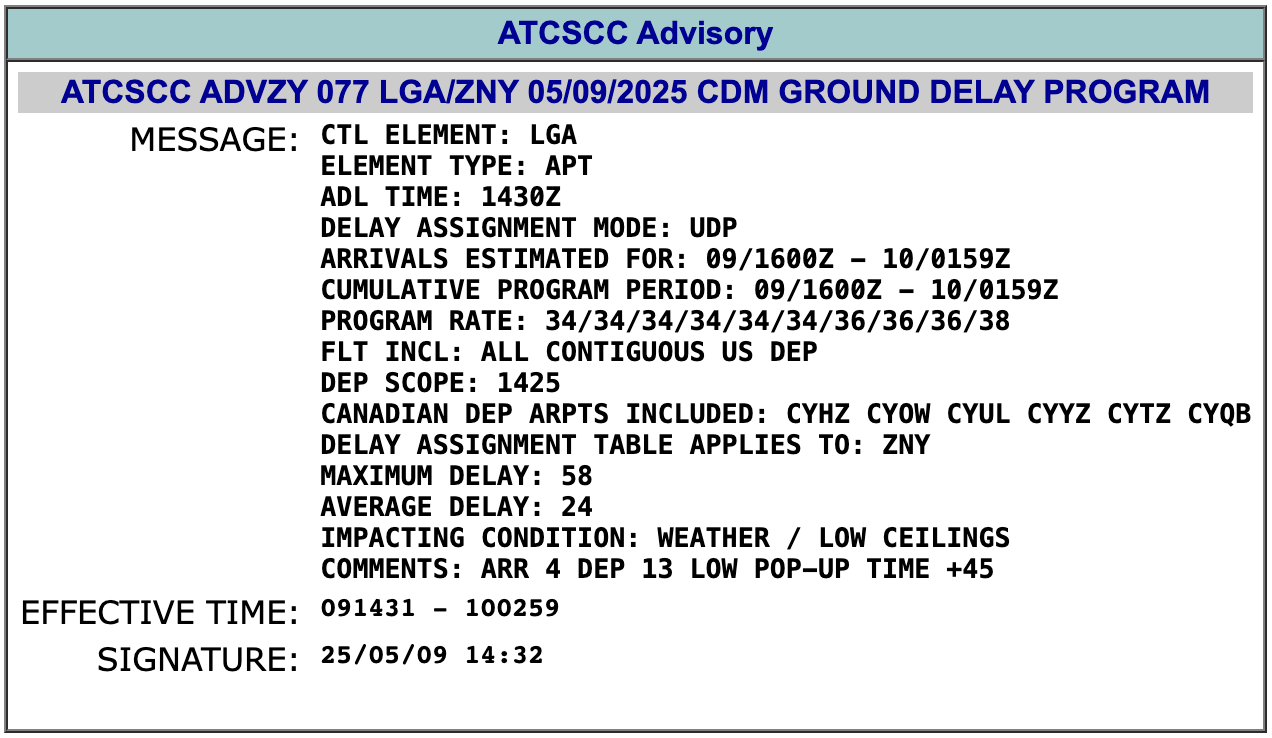
\includegraphics[height=2.2in]{media/gdp_advisory.png}
    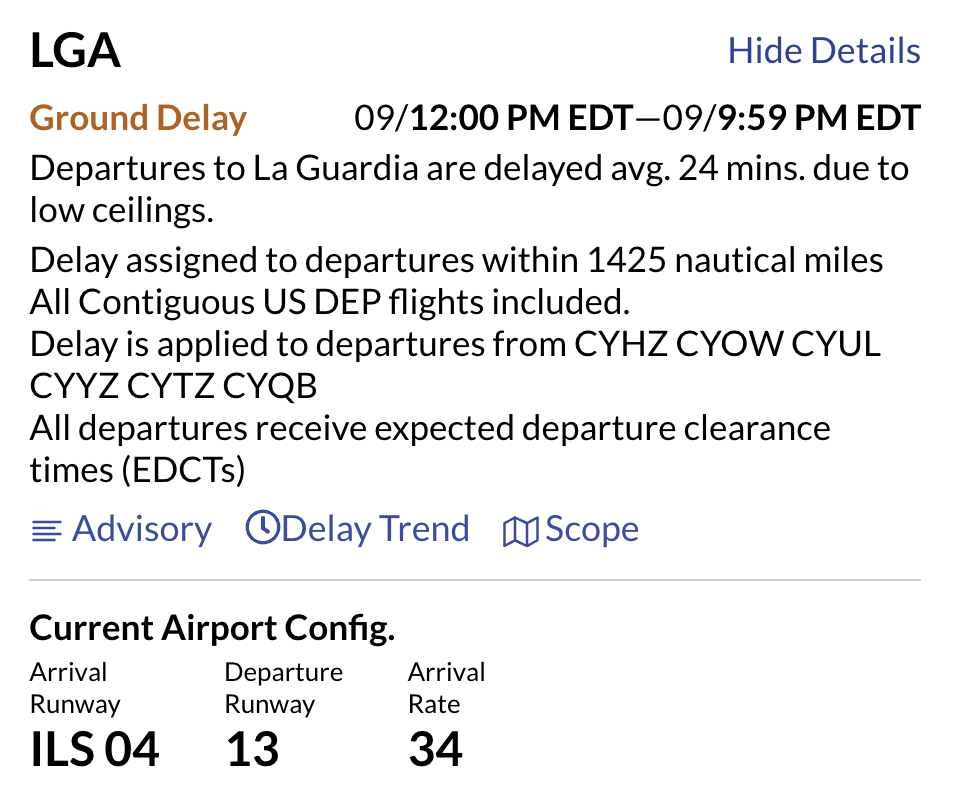
\includegraphics[height=2.2in]{media/gdp_meaning.png}
    \caption{GDP applied to flights headed to LGA due to weather on May 9th, 2025.}
    \label{fig:gdp-example}
\end{figure}

For completeness, we will also describe some other common TMIs, roughly sorted by their general purpose. First, initiatives to create space, both physically and temporally, between aircraft generally fall into one of several categories. Altitude-based TMIs may be used to separate traffic flows close to each other, by imposing altitude restrictions at various phases of a flight, both at arrival and departure, as well as en-route. Miles-in-trail and Minutes-in-trail (MINIT) work along a slightly different axis, where aircraft along a common flow of traffic are directed to be spaced out by at least some minimum physical or temporal separation, depending on what sensor information is available and the spacing required \cite{faa_tfm_prez_2009}.

Other traffic initiatives work more directly to manipulate the timing of arrival and departure phases of flights. For example, fix balancing may change these times to even out traffic at the arrival or departure endpoint of a flight. Similarly, flights may be held on the ground at the departure endpoint, as we saw earlier with GDPs, and also in the air at the arrival endpoint, which is known as airborne holding. The locations of flight endpoints might also changed by reroutes or diversions, which may happen both before departure and en-route. In some more extreme cases, Ground Stops (GSs), where certain flights are held on the ground until the GS is lifted instead of just delayed as in GDPs, may be even necessary \cite{faa_tmi_2024}.

Although we will not discuss these TMIs in more detail, the main takeaway is that even localized disruptions can become globalized because of the actions taken as a result of necessary responses. Therefore, it is natural to first separate our disruptions into two categories. We will say that disruptions that originate completely outside of the system and are, such as weather effects reducing an airport's capacity, are exogenous disruptions. On the other hand, disruptions that are created as a result of actions taken within the system, such as flight delays due to the implementation of GDP in response to an exogenous effect, will be referred to as endogenous disruptions. While these two can be related, as in our GDP example, the effects of disruptions only accumulate in one direction: exogenous disruptions can cause and exacerbate endogenous disruptions, but not the other way around. Because of this, it makes sense to break up observed disruptions into causally linked components and work out their dependency structure, as we will see later.

\subsection{Other Factors}

As we saw earlier, exogenous disruptions from natural events like convective weather can lead to endogenous disruptions from traffic management initiatives raised in response. One natural question to ask is then, how other stakeholders may be affected by both of these. We can also classify these as endogenous effects, but it makes sense to distinguish who is responsible for said effect, which may be traffic managers, or airlines. In the case of airlines, there is potential for further disruptions that are a result of less than optimal processes in place to respond to their flights being delayed. For example, this could be not having allocated crew and fleet resources in a sufficiently robust manner \cite{dot_penalizes_2023}, or being unable to adapt quickly enough to changing situations. In this sense, we can see that there is also a sort of response to the disruptions here, only this time on the part of airlines instead of traffic managers. 

For instance, one common response is to cancel flights that the airline believes they will be unable to service, for some reason or another \cite{bts_causes_2024}. Although airlines do sort of exert pressure on traffic managers through the demand they create with scheduled flight operations, during a disruptive event on a day to day basis, their actions are still more in response to what happens from ATM actions. Therefore, with this dependency structure in mind, we can see that we have several steps that occur mostly in order conceptually, which are weather, traffic manager responses, then airline responses. 

At each step, we can accumulate more severity, so to speak. The weather events initiate disruptions, traffic managers may or may not respond optimally, and then airlines may or may not respond optimally to what the situation is once it ends up at them. This order is important because failures often only occur above some threshold level of severity, in some sense, so there may be less than optimal processes further along the pipeline that are not discovered because the processes before them are doing alright, but in slightly more severe events may manifest and lead to serious unexpected issues. 

We will also note that there are other factors that could fall under the exogenous step, and be treated as a given that is not really a response to anything necessarily in the network. For example, airports undergoing large construction projects may have reduced performance compared to normal operation \cite{faa_construction_2025}. Staffing issues for facilities within the NAS may also pose challenges that may not be immediately fixable \cite{faa_newark_staffing_2025}. Similarly to weather, it may be difficult to exactly represent how these other factors may affect different parts of the network. 

\subsection{Taxonomy Outline}

Now that we have a better idea of the flow of disruptions and associated responses in our system, we can begin to put together a taxonomy of disruptions and responses, which will help us better understand how historical failures, which may seem very different at first glance, are intrinsically related below the surface. It is important to stress that this will not attempt to be any sort of comprehensive classification, but rather a collection of ideas from our reasoning above placed in a coherent framework to motivate further study.

\paragraph{Dependency structures} First, we need to generate a dependency structure for the major events that combine to form the overall observed disruption. This should incorporate both exogenous and endogenous effects. For the exogenous disruptions, since we consider them to be essentially uncontrollable environment parameters, we should also consider the frequency and severity of the event, both expected based on domain knowledge, and historical based on past data, if any. 

\paragraph{Severity} We can further break down severity into a few different parts. The first is the persistence of the event, or how long it was in effect. Longer events are generally of more concern than shorter ones, given the same pure severity level. Here, by pure severity, we are just referring to the direct instantaneous effect of the event without considering any temporal aspects. In practice, however, pure severity and length tend to be relatively well correlated. Moving on from temporal considerations, a third aspect to consider is the spatial size of the event. Roughly speaking, this would refer to whether the event was local to a single node and a just few nearby nodes, or if spanned a significant part of the overall network. If the event can be split into several sparse, more localized components, then it may be more natural to consider it that way instead. There are other things that could be considered here, but for now, these are most relevant.

\paragraph{Frequency} In terms of frequency, we are both interested in frequency in the usual sense, or how often said event occurs, and what we will call predictability. This is essentially just to say that there is a difference between infrequent events that happen completely randomly, and infrequent events that occur on a regular basis. Likewise, not all frequent events are created equal. For example, we might know that certain months are more prone to severe storms than others, and this can be something that is modeled in. 

\paragraph{Simplified example} Let us use a slight extension of our guiding example in \cref{ch:atrds} to give us something concrete to work with. In this hypothetical scenario, we will suppose that due to an ongoing weather event at LGA, the airport arrival and departure capacities were greatly lowered, and a ground delay was implemented for scheduled incoming flights. For one airline, these delays propagated throughout the network, because of insufficient fleet reserves, and led to a large number of canceled flights for the day. The weather event was unusually severe and persistent, and was not something that had been commonly seen up until now. However, it was mostly localized to the airspace around LGA, and did not directly affect the operations of most of the other airports in the network that were not nearby.

In this simplified example, we can separate the overall disruption into three components that follow a linear dependency structure. First, the weather event reducing capacity at LGA is the exogenous disruption. Then, the ground delay is an endogenous disruption generated in response. Finally, the airline flight cancellations is the third component. In our weather event itself, we can see that it is relatively well localized, but is severe both in terms of pure severity and persistence. The weather event is infrequent, and since it is a newly observed type of event, we consider it to be unpredictable by default. 

Moving on from categorizing the initial exogenous disruption, we can also analyze the accumulated disruption as we move through the dependencies that ultimately led to the hypothetical failure. Here, there are a few groups of possibilities. One would be that the traffic management was done optimally, in which case this failure would reveal a weakness in the airline processes that had not been exposed up until this point, due to a continuance of only nominal conditions. Similarly, it is also possible that the airline responded optimally within their constraints, and that improvements could have been made to the traffic management response, and of course, everything in between, as real scenarios are generally not so cut and dry. 

\paragraph{Stakeholder perspectives} Assessing this allocation of accumulated disruption across nodes in the dependency graph can be challenging and often subjective, though not necessarily impossible. However, we will instead focus on a variational approach, where we assume the perspective of the relevant stakeholder to a particular node, and model the rest of the nodes as autonomous processes acting according to a defined set of behaviors based on prior belief. In our hypothetical example, this could be building a simulation where the airline response can be controlled, but all else are held constant, in order to assess how different strategies might have performed, and if there was any improvement to be made leading up to the failure. We can also consider the entire system to be autonomous, in which case we would arrive at the problem of inferring the initial exogenous disruptions, which is the scenario our work in \cref{ch:atrds} would fall under.

\section{Historical Case Studies}

We will now apply our taxonomy to real historical examples, which may help in motivating the structures and perspectives to build our simulations in mind with. The point is to show that by analyzing these scenarios in this manner, we can also get a better idea of where improvements could be made, so that we can decide which parts of the model should be controllable and which should not, as well as parameters to represent the disruption.


\paragraph{Chronically delayed flights} The Bureau of Transportation Statistics defines chronically delayed flights as ``flights with more than 50\% delayed arrivals of more than 30 minutes'' \cite{bts_chronic}. Historically, legal and punitive action, of hundreds of thousands of dollars in penalties, have been taken against carriers such as Southwest Airlines and Frontier Airlines for operating chronically delayed flights, as these are considered evidence of illegally unrealistic scheduling that can negatively affect both passengers and industry standards \cite{southwest_chronic_2025}. By definition, these are high frequency events that are predictable, at least at the point when they become classified as such. Since the impact on an individual basis is limited to a single flight, they are also low severity, but can add up if it is a common occurrence across an airline's routes. Since this is specifically caused by airline scheduling practices, we don't have an exogenous event or traffic management response for risk to accumulate through, therefore our dependency graph only involves the airline. In some sense, the airline's poor scheduling practices could be considered an exogenous event in this case.

\paragraph{Logan snow and ice delays} Next, we return to a more standard exogenous effect from poor weather. At Logan International Airport, snow and ice caused hundreds of flights to be delayed one Saturday in January 2025, even though the storm was relatively localized and not a major event in the surrounding area. A ground delay program was initiated because of the weather to manage capacity. However, because the weather event moved South over time, other nodes began to be affected, which led to thousands more delays and cancellations in later days \cite{nbc_logan_2025}. Here, we can clearly see the dependence structure, progressing linearly from winter weather to traffic management response as a GDP, to disruptions for flights in the network. Note that we can see two aspects of severity here: first, that the storm system had a localized effect mostly contained to a single area, but that same storm system ended up having a much larger effect as it moved and was no longer localized. The storm appeared to be in line with usual winter weather, but is still a relatively infrequent event, so we can say that it is predictable but low frequency.

\paragraph{Newark radar outages} We can also observe a similar effect at a single node, although this time, due to a non-weather effect. In 2025, Newark Liberty International Airport (EWR) suffered multiple incidents of radar and connection outages that caused significant disruption to capacity, as well as staffing issues as a secondary effect. These events sometimes only lasted a short period of time, but still eventually led to widespread effects as the disruption propagated throughout the network \cite{apnews_newark_2025}. This scenario is similar to the previous one. However, one fundamental difference is that weather cannot be addressed directly, as it is something that is totally out of our control, while air traffic control systems in need of repair is something that can be done. Another key difference is that storms are generally higher length events, while we can see here that radar outages may have much shorter length.

\paragraph{Southwest scheduling crisis} Finally, we once again turn our attention to the Southwest Airlines scheduling crisis during winter storms in 2022, which we've discussed earlier multiple times \cite{cnn_southwest_2022}. We note that the exogenous event in this case was low frequency but relatively predictable. The severity was high, both in terms of duration length, pure severity, and spatial size. It's difficult to say if the traffic management response accumulated significant severity, but because Southwest was specifically affected far more than other airlines, it is likely that it was more of an issue with their response specifically. This sort of exogenous event that exposes some weakness in an airline's systems also has shown up often in the past, such as with Southwest again in 2021 \cite{cnn_southwest_2021}, American Airlines in 2018 \cite{usatoday_aa_2018}, and Delta in 2017 \cite{cnn_delta_2017}. A recurring theme seems to be that difficulties in IT systems tend to exacerbate issues, which means that for these cases, it would make sense to focus on airline responses as a controllable aspect of the simulation. Additionally, incorporating reaction speed could be a reflection of how well the IT systems work, and we would also expect to see that a more reactive response would likely perform better than one that is slower. 

\paragraph{Delta IT outages} We will also include one more related example of Delta in 2024, where the disruption was directly in IT systems as a major outage during a failed CrowdStrike software update, leading to thousands of canceled flights \cite{cnbc_delta_crowdstrike_2024}. Although this is related to the previous examples we just discussed, it is slightly different in that the disruption was essentially exogenous, but bypassed every other step to directly affect airline operations. In cases like these where reacting is not particularly feasible, we could instead try to focus on modeling recovery after the fact.

\section{Summary}

In this chapter, we first introduced the primary object we are interested in, the National Airspace System, and covered the hierarchical structure through which air traffic control and management operate within it. Additionally, we briefly went over simulation considerations, and discussed what use cases current state-of-the-art simulators may not necessarily cover completely. Then, we introduced a taxonomy of weather disruptions and responses, breaking them down into dependency structures and multi-faceted notions of frequency of severity, as well as stakeholder perspective. Finally, we applied our taxonomy to a few real world historical scenarios for demonstration.
\chapter{Defining and Quantifying Failures}
\label{app:risk}

Earlier in \cref{ch:atrds}, a particularly skeptical reader may have noticed several challenges that we did not spend much time discussing, that are inherently tied the stochastic nature of our system. Thus, this chapter will be focused on addressing these challenges, to help us more concretely define failures, and quantify the extent to which we should be concerned about them. We will introduce the concept of risk measures in the univariate case, to first illustrate how we can express our tolerance for risk of failure. Then, we will move on to the more relevant multivariate case, where we discuss some extensions along both the spatial and temporal axes, and will attempt to bridge all of our concepts together under the unifying idea of distortions. Finally, we will end with some brief discussion on how we can account for the network structure of our data in everything we had just outlined.

\section{Guiding Questions}
\label{sec:risk-questions}
For now, let us suppose we have some black-box system, which given an input $z\in \mc Z$, will spit out a value of interest $x=f(z)$, where $x\in \mc X$. We will use this as the canvas for a few guiding questions, to help set the stage for the rest of this chapter.

\paragraph{Why is stochastic harder than deterministic?} We will start with the deterministic case, which would correspond to removing all sources of randomness from our air traffic simulation. Then, if we decide that we have some failure region $\Omega\subseteq \mc X$, we can simply check if the deterministic value $x$ returned by $f$ falls within $\Omega$. However, if $f$ is not deterministic, the question becomes a little more complicated. Instead, for the same input $z$, we could query our system $n$ times and receive $n$ different outputs $x^{(1)},x^{(2)},\ldots, x^{(n)}$, where only some lie in $\Omega$ and the rest do not. Even if we knew the structure of $f$ a priori, we would still have this problem. Furthermore in the black-box case, introducing stochasticity in this manner means that more data is required to understand the shape of $f$, as we can no longer say that a single data point is sufficient.

\paragraph{What exactly is a failure?} Let us be a bit reductive and only consider the case of an arrival time for a single flight, and suppose that the random value $x$ we were discussing now quantifies the delay in minutes. We had previously used 15 minutes, based on federal guidance, as a threshold for delays, so we will consider all values above that to be our failure region. Earlier, one example we had used is considering the probability that $x$ falls above the threshold, or in other words, using the language of catastrophe modeling, the Occurrence Exceedance Probability (OEP). Similarly, we could extend this to multiple occurrences and consider the probability some sort of aggregation, such as average, falls within the failure region. As one might expect, this is known as Aggregate Exceedance Probability (AEP). This sort of solves our problem of converting stochasticity into a more familiar deterministic setting, but is a little inflexible, and perhaps not fully representative of the extent of a failure. Under the exceedance probability framework, or anything similar, we only consider if our samples used to estimate the probabilities lie within the failure region or not, so a delay of 20 minutes would be treated the same as a delay of 200 minutes, even though they are very different. It is possible to vary the threshold and consider all the results, but we might still want to consider an approach that takes the severity of a failure into account more directly. 

\paragraph{How can we specify risk tolerance?} Another weakness with the approach we just discussed is that there isn't really a natural way to specify your tolerance for risk of failure, as we specify the threshold first and then get a probability, instead of the other way around. Naturally, there are so-called risk measures that allow us to do this. For now, let's imagine that we have many samples of delay values in front of us, and that we decide that our tolerance for risk is 5\%. We'll discuss exactly what this means in more detail later. Then, suppose we sort them from smallest to largest, and take the mean of the worst, or largest, 5\% of them. This idea of averaging the worst values is known as the Tail Value at Risk (TVaR). Similarly, we could take the smallest value in that group, in which case we would obtain the Value at Risk (VaR). Then, how does this relate to our questions about failure? First, most related to our previous discussion on exceedance probabilities is the VaR, as it is essentially just the inverse problem of OEP, where we start with the probability, and want to obtain the associated threshold. To check for failure, we could compare this value against a pre-defined threshold for failure. On the other hand, TVaR goes beyond this and also includes some measure of the severity of failures in a region. As we will see later, there plenty of other ways we can go about measuring the risk-aware performance of our system that may be of interest as well.

\paragraph{Is a single number really good enough?} So far, we have only been working with the idea of a single value $x$ that we can use to determine whether or not an event is a failure, and to what extent. However, in real world scenarios, we are often working with multiple variables, which introduces a trade-off between granularity and interpretability. For example, one natural case is considering the delay data at each airport in our network. If we somehow combine all of our information into a single number, then interpretability is achieved, but we may lose some of the granular information in the process. On the other hand, if we maintain full granularity, such as by having a full dimensional vector, then we lose interpretability, as it's much harder to reason about what's going on and more difficult to visualize, compared to fewer numbers. As we will see, it takes some care to express risk associated with inherently multivariate results in an interpretable manner. Also relevant, though less covered in this chapter, is the inherent network structure to our data, which can help guide our decisions here.


\section{Risk Measures}
\label{sec:risk-intro}

Now, we will go further into our guiding questions on defining failures through a quantitative measurement of risk. For now, we will stick to the univariate case, to develop some relevant background before we move on to multiple variables. Here, our goal is to understand how we can bridge the gap between the stochastic and deterministic worlds through risk measures that allow us to collapse probability distributions into values of interest. In this section, we will introduce some background to use in later discussion, from existing literature on risk measures in \cite{Mildenhall_Major_2022, Artzner_Delbaen_Eber_Heath_1999, risks11110194, wirch_hardy_2003}, and so we defer to these sources for a more in-depth development.

\subsection{Preliminaries}

Let $\rx\sim \pxdd$ be a continuous random variable, where $\pxdd$ is the probability density function (PDF) of $\rx$, and with $x\in \mc X$ denoting observations of $\rx$. For simplicity, we will take $\mc X = \RR_{\ge0}$, or the nonnegative reals. We will make the usual regularity assumptions. Additionally, although we will not cover the discrete case, the main idea of the ideas here are roughly the same. Now let $\Fxdd$ and $\Sxdd$ denote the cumulative distribution function (CDF) and survival function (SF) of $\rx$, respectively. Just to review:

\begin{definition}[Cumulative Distribution Function and Survival Function]
    The relationship between the CDF and SF is given by
    \begin{equation}
    \Fxd{x} = \PR{}{\rx\le x} = \int_{0}^x \pxd{t}\,dt = 1-\int_{x}^\infty \pxd{t}\,dt = \PR{}{\rx > x} = \Sxd{x}.
\end{equation}
\end{definition}

We can take analogous definitions for $\ry$ and $y\in\mc Y$. For now, and the rest of this section, we will use these random variables to denote some sort of failure-sensitive quantity, where higher values are worse than lower values. For example, this could be the service time of an airport, or the delay of a flight. 

\paragraph{Risk preferences} First, let us consider the idea of risk preference. Suppose we have $\rx$ and $\ry$, which give us two different distributions of failure-sensitive quantities. Although we have not defined any systematic ways of doing so yet, we might imagine that we have some system to assign a preference to one risk, in this case the $\rx$ and $\ry$, over another. We say that $\rx \succeq \ry$ if $\rx$ is preferred over $\ry$, and vice versa for $\rx \preceq \ry$. It is possible that $\rx\succeq \ry $ and $\rx \preceq \ry$ are both true, in which case $\rx$ and $\ry$ are risk neutral and we do not prefer one over the other. This does not necessarily imply $\rx$ is equal to $\ry$, however. 

\begin{proposition}[Risk preference properties]
    We have three axiomatic properties for risk preferences:
    \begin{enumerate}
        \item \textbf{Completeness}: at least one of $\rx \succeq \ry$ or $\rx\preceq\ry$ is always true.
        \item \textbf{Transitivity}: if $\rx \succeq \ry$ and $\ry\succeq \rz$, then $\rx\succeq \rz$.
        \item \textbf{Monotonicity}: if $\rx \le \ry$ almost surely, then $\rx \succeq \ry$.
    \end{enumerate}
\end{proposition} 
In words, completeness and transitivity just guarantee that we are always able to compare risks in a logically consistent manner. Monotonicity essentially just captures the idea that we should prefer lower values to higher values.

\paragraph{Risk measures} Now we define a risk measure $\rsd$ as a function of a random variable $\rx$, which will help us convert our inherently stochastic quantity into something deterministic that captures both the severity of a potential failure and the associated uncertainty. In doing so, we will also be able to express our risk preference in a systematic manner. In other words, we will be able to quantitatively say what $\rx$ being less risky than $\ry$ means, according to some internal definition of risky. Here, the preference based definition is quite intuitive, and says exactly that:
\begin{equation}
    \rx \succeq \ry \iff \rs{x} \le \rs{y}.
\end{equation}
This formulation also immediately satisfies the first two properties, completeness and transitivity, because of the natural ordering of $\RR$. Monotonicity does not necessarily hold for all choices of $\rsd$, but we will see that it is usually not a problem for the constructions we are interested in. 

\paragraph{Examples} The most obvious example of a useful risk measure is simply the expected value $\rs{\rx}=\EX{}{\rx}$. However, in aggregating the risk distribution in this way, we lose a lot of information about what it looks like, particularly in its variability. Roughly speaking, we should consider risks that are more volatile to be less preferable to risks that are more well behaved and tightly concentrated around the mean. 
\begin{example}[Moment-based Risk Measures]
    Therefore, some risk measures directly attempt to directly penalize this as
    \begin{align}
        \rs{\rx} = \EX{}{\rx} + \lambda\Var\pars*{\rx},\\
        \rs{\rx} = \EX{}{\rx} + \lambda\SD\pars*{\rx},
    \end{align}
    where $\SD\pars*{\rx}=\sqrt{\Var\pars*{\rx}}$ denotes standard deviation, and $\lambda$ is a given constant.
\end{example}

\subsection{Coherence and Convexity}

\paragraph{Risk measure properties} Before we move on, we will introduce a few more useful properties of risk measures.
\begin{itemize}
    \item \textbf{Monotonicity}: if $\rx\le\ry$ almost surely, then $\rs\rx \ge \rs\ry$
    \item \textbf{Sub-additivity}: $\rs{\rx+\ry}\le \rs\rx+\rs\ry$
\end{itemize}
Now, if a risk measure $\rsd$ also satisfies the following two properties, it is also coherent.
\begin{itemize}
    \item \textbf{Positive homogeneity}: $\rs{\alpha\rx}=\alpha\rs\rx$ for $\alpha\ge 0$
    \item \textbf{Translation invariance}: $\rs{\rx+c} = \rs\rx+c$
\end{itemize}
If, instead it only satisfies the following property in addition to the first two, it is convex.
\begin{itemize}
    \item \textbf{Convexity}: $\rs{\lambda\rx+(1-\lambda)\ry}=\lambda \rs\rx+(1-\lambda)\rs\ry$.
\end{itemize}

\subsection{Quantile-based Measures}

\paragraph{Value at Risk} One natural idea is to ask at what level do the worst, say $5\%$, of values start at? We can answer this by simply taking the inverse of the CDF, so that $\Qxd{\pi} = \Fxdinv{\pi}$ and $\Fxd{\Qxd{\pi}} = \pi$. We will note that we are assuming $\Fxdd$ has a well defined inverse for simplicity, but the definition is also similar if that is not the case. With our $5\%$ example, $\pi$ would be $95\%$. As it turns out, this is precisely the Value at Risk (VaR) definition we introduced earlier: we choose some risk level, say $\pi=95\%$, and calculate $\Qxd{\pi}$, which gives us the value where we start to get into the worst $1-\pi=5\%$ of outcomes.

\begin{definition}[Value at Risk]
    The Value at Risk (VaR) risk measure is given by
    \begin{equation}
        \rs{\rx} = \VaR{\pi}{\rx} = \Qxd{\pi}.
    \end{equation}
\end{definition}

The choice of $\pi$ allows you to set your risk tolerance, where higher values of $\pi$ correspond to higher tolerances, and vice versa for lower values. For now, we are using $\pi$ to avoid confusion with the PDF $\pxdd$, but later we may instead just use $p$.

\paragraph{Tail Value at Risk} Often, it also makes sense to capture what the tail actually looks like, instead of a single value from the beginning of the tail. For example, if there is a $4\%$ chance of having a five hour delay and a $96\%$ chance of zero delay, then $\VaRd{95\%}$ would still give you zero delay, even though you might be worried about the non negligible probability of an extremely high delay. To express this, the Tail Value at Risk (TVaR) extends the idea of VaR, but instead calculates the average of the worst outcomes. For a given risk level $\pi$, we have equivalent definitions for this risk measure.

\begin{definition}[Tail Value at Risk]
    The Tail Value at Risk (TVaR) risk measure is given by 
    \begin{align}
        \rs{\rx} = \TVaR{\pi}{\rx} &= \EX{}{\rx \given \rx \ge \VaR{\pi}{\rx} }\\
        &= \frac1{1-\pi}\int_{\VaR{\pi}{\rx}}^\infty t\pxd{t}\,dt\\
        &= \frac1{1-\pi}\int_{\pi}^1 \VaR{s}{\rx}\,ds.
    \end{align}
    Other names for TVaR in the literature are Conditional Value at Risk (CVaR) and Average Value at Risk (AVaR).
\end{definition}
TVaR is also sometimes used interchangeably with Conditional Tail Expectation (CTE) and Worst Conditional Expectation (WCE) for continuous random variables, but these are not equivalent for discrete ones. We will not go into that here, but leave further investigation to the presumably interested reader.

\paragraph{Empirical versions} When we are not given the risk distribution $\pxdd$ in closed form, but are able to generate samples from it, we can estimate the VaR and TVaR as follows.

\begin{example}[Empirical VaR and TVaR \cite{cakmak2020bayesianoptimizationriskmeasures}]
    Suppose we have a sample of $n$ values with order statistics denoted as
    \begin{equation}
        x_{(1)} \le x_{(2)} \le \cdots\le  x_{(n)},
    \end{equation}
    then the empirical VaR and TVaR at risk level $\pi$ are given by the analogous
    \begin{align}
        \eVaR{\pi}{\rx} &= x_{(m)} \\
        \eTVaR{\pi}{\rx} &= \tfrac{1}{n - m+1}\sum_{i=m}^{n} x_{(i)} ,
    \end{align}
    for $m=\lceil \pi\cdot n\rceil$, where $\lceil\cdot\rceil$ is the ceiling function.
\end{example}

This sort of Monte Carlo integration is also applicable to other risk measures that we will see later, but we will not be discussing it in depth.

\subsection{Distortion Functions}

Notice that VaR and TVaR still have something in common with just taking the expected value. Namely, we are still essentially taking a weighted average of the possible outcomes, it's just that in the expected value case, we just use a weighting given by our density $\pxdd$, whereas VaR and TVaR will distort the density in some way to express our risk preference. VaR places full weight on a single point, while TVaR redistributes the weight across the tail beyond a point. This motivates the introduction of so-called distortion functions, which are defined as follows.

\begin{definition}[Distortion Function]
    An increasing $g:[0,1]\to[0,1]$ is a distortion function if $g(0)=0$, $g(1)=1$, and $g(s)\ge s$ for all $0\le s\le 1$. 
\end{definition}

Often, $g$ is taken to be concave to provide some convenient properties, and so we will assume this to be part of the definition for the rest of our development. 

\subsection{Spectral Risk Measures}

Now, we can see how these distortion functions can be used to generate risk measures with useful properties under a single unifying framework.

\begin{definition}[Spectral Risk Measure]
    The spectral risk measure (SRM) associated with a distortion function $g$ is given by 
    \begin{equation}
        \rs{\rx}=\int_0^\infty g(\Sxd{t})\,dt = \int_0^\infty tg'(\Sxd{t})\,d\Fxd{t} = \EX{}{\rx g'(\Sxd{\rx})},
    \end{equation}
    assuming the reasonable tail decay condition $tg(\Sxd{t}) \to 0$ as $t\to\infty$.
\end{definition}

Unlike VaR and TVaR, an empirical estimation is a bit more involved, but still possible, though we will not go into that now\cite{pandey2019estimationspectralriskmeasures}. Here is an alternative definition that more directly illustrates the re-weighting process.

\begin{definition}[SRM via Spectral Weight Function]
    An equivalent definition for our spectral risk measure is as follows:
    \begin{equation}
        \rs{\rx} = \int_0^1 q(p) g'(1-p)\,dp = \int_0^1 q(p)\phi(p)\,dp ,
    \end{equation}
    where $p = \Fxd{t}$ and $t=q(p)=\VaR{p}{\rx}$, so that $d\Fxd{t} = dp$. 
\end{definition}

Here, $\phi(p) = g'(1-p)$ is referred to as the spectral weight function, as it describes how much weight our spectral risk measure places on the outcome $q(p)=\VaR{p}{\rx}$. Then, as described earlier, we have the following:

\begin{example}[SRM Formulation of VaR]
    Consider the distortion function $g(s) = \mbm{1}_{s>1-p}$, or the step function that is $0$ for $s<1-p$ and $1$ for $s\ge p$. Then $g'(s)=\delta(1-p)$, where $\delta(\cdot)$ is the Dirac delta function, and so $\phi(s) = g'(1-s) = \delta(p)$. Therefore, we have
    \begin{equation}
        \rs{\rx} = \int_0^1 \VaR{p}{\rx}\cdot \delta(p)\,dp = \VaR{p}{\rx}.
    \end{equation}
\end{example}

\begin{example}[SRM Formulation of TVaR]
    Consider the distortion function $g(s) = \min(\tfrac{s}{1-p},1)$. Then $g'(s)$ is equal to $\tfrac1{1-p}$ for $s\le 1-p$ and is zero otherwise, so
    \begin{equation}
        \phi(s) = g'(1-s) = \begin{cases}
            \frac1{1-p} & s\ge p \\
            0 & s< p,
        \end{cases}
    \end{equation}
    and applying this weighting in our integral yields
    \begin{equation}
        \rs{\rx} = \int_{p}^1 \VaR{p}{\rx}\cdot \frac1{1-p}  = \TVaR{p}{\rx}.
    \end{equation}
\end{example}

For the remainder of this section, we will not focus too much on the technical details of developing distortion functions and spectral risk measures. Instead, we will mainly work with SRMs at a high-level, interpreting them as a principled re-weighting of outcomes according to a user's risk preference. To this end, the previously given examples of VaR and TVaR will be helpful to keep in mind.


\section{Multivariate Extensions}
\label{sec:risk-multi}

So far, we have mostly been discussing risk regarding a single random variable $\rx$. However, in our air traffic problem, we actually have multiple different axes on which individual risks, such as flight delays, are naturally divided along. While there is related work in generalizing univariate risk measures to the multivariate case, such as in \cite{Shushi_Yao_2020} and \cite{RePEc:hal:wpaper:hal-01831481}, we will consider those details outside of our scope for now, and instead focus on the main ideas behind extending to the multivariate case.

\paragraph{Spatial axis} The first is due to the inherent network structure of the problem. Let us forget about temporal considerations for a moment, and pretend that we have a single value for each airport, such as mean delay per node, that represents their individual risk. Naturally, we know that these are all correlated. Now suppose we tried to naively reduce our problem to the univariate case by aggregating all of our delays together into a single mean delay for the whole network. One benefit is that we improve interpretability, as a single number is much easier to understand than many, especially in our case where we may have thousands of different airports. However, by combining all of our granular information in this way, we destroy the inherent network structure to our data. Additionally, not all delays are created equal, and our risk tolerance may be different for certain nodes or sections of the overall network based on our prior beliefs about each specific airport. However, including the full granularity of the data is perhaps not the right answer either.

\paragraph{Temporal axis} The second is due to the inherent temporal structure of the problem. Focusing on a single airport for a moment, it is possible that our delays vary depending on time of day, as the data comes from a time varying process. For example, one common phenomenon is that less delay may be observed in the beginning of the day, but it steadily increases for flights later in the day as delays propagate throughout the network. Then, as we can see, simply taking a mean may not be fully representative of the data, as a day with a constant moderate delay of 15 minutes is very different from a day with spikes of 150 minute delays occurring 10\% of the time. Maintaining full granularity, we could take this to be a vector containing the full delay profile of this particular node for the day, which may include hundreds of flights. Once again, we reach the question of how we can meaningfully collapse this into a more interpretable representation.

\subsection{Dimensionality}

For now, we will return to the simplified case for the spatial axis, and return to the temporal axis later. For this setup, let us suppose we have a network $G$ with vertex and edge sets $V$, $E$, respectively. Enumerate the vertices in $V$ as $v_1,v_2,\ldots,v_n$, and include an edge $e_{i,j}$ in $E$ if an edge exists between $v_i$ and $v_j$. Then, similarly to before, equip each node $v_i$ with random variable $\rx_i$ which we will use to analyze the risk of each node and the network as a whole.

\paragraph{Univariate aggregation} First, we will compare some methods to aggregate these risks into a single risk or value. These will be easier to use, but perhaps more restrictive than our later inherently multivariate discussions. However, since univariate is just a special case of multivariate, it will still be useful to motivate our main ideas here.

\paragraph{Weighted average} One way to do so is by taking a weighted average of our existing risks.

\begin{example}[Weighted Average Aggregation]
    Let $w_i$ be an importance weight placed on node $v_i$. Then, we can define a network risk
    \begin{equation}
        \rx = \frac{\sum_{i=1}^n w_i \rx_i} {\sum_{i=1}^n w_i}.
    \end{equation}
\end{example}

We can choose the weights $w_i$ in various ways. For example, if the $w_i$ are simply chosen to be the number of flights that have an endpoint at node $v_i$, and the original $\rx_i$ are the mean flight delays for each node, then this $\rx$ is essentially just a straight average of all flight delays across the network. It may also make sense to place heavier weight on more important nodes. For example, in a hub and spoke network structure, delays at a central hub may be of greater interest. However, notice that this aggregation transformation does not preserve risk measures, so it is not guaranteed that 
\begin{equation}
    \rs{\rx} = \frac{\sum_{i=1}^n w_i \rs{\rx_i}} {\sum_{i=1}^n w_i}
\end{equation}
also holds, as not all risk measures have the linearity property like expected value does. In fact, if we choose an SRM for $\rho$ with a concave distortion function, then it is coherent and therefore subadditive, so we could only say
\begin{equation}
    \rs{\rx} \le \frac{\sum_{i=1}^n w_i \rs{\rx_i}} {\sum_{i=1}^n w_i}
\end{equation}
Then, how can we robustly combine information from each of the individual risk measures without having to work with an aggregated risk, which may be more difficult to analyze?

\paragraph{Node-level distortions} Let us first consider a simple example, where we choose $\TVaRd{p}$ as our risk measure, and apply it to each node as $\TVaR{p_i}{\rx_i}$. Then, a simple way to express our risk preference on a node level is to vary the risk level $p_i$. Nodes that are considered to be more critical should use a higher $p_i$ to distort their distributions more toward the right tail, while those that are less critical can set their level at lower values. Note that at risk level of zero, the TVaR and expected value are equivalent. However, our risk measures are still inherently decoupled with this structure, and we would still need to combine them once again after the fact somehow. It is then clear that this pattern of aggregation will always have limitations if we want to reduce dimension this aggressively. However, with this node-level approach, we can maintain slightly better expressivity compared to before, because of the more interpretable method of setting risk tolerance levels instead of having to choose weights without as direct of an interpretation. To generalize this slightly, we can work directly with distortions.

\begin{example}[Node-level distortions]
    Select distortion functions $g_i$ with associated SRM $\rho_i$ for each node. Then, compute each $r_i = \rsg{i}{\rx_i}$, and aggregate results into a single 
    \begin{equation}
    r = \rho^*(\rx_1,\ldots,\rx_n) = \frac{\sum_{i=1}^n w_i \rsg{i}{\rx_i}} {\sum_{i=1}^n w_i} = \frac{\sum_{i=1}^n w_i r_i} {\sum_{i=1}^n w_i}
    \end{equation}
\end{example}

\paragraph{General pattern} In the two examples above, we can see some steps that occur in different orders. One is applying an aggregation function, say $g(\cdot)$, that takes care of the dimensionality reduction goal. This could be a weighted average, as we saw before, or some other function, such as the maximum function. The choice of aggregation function is somewhere risk preference can be expressed. For example, choosing to use an average represents a greater risk tolerance than maximum, which represents a lower risk tolerance more focused on the worst-case outcomes. Another step is applying a risk measure $\rho$, and the order of these steps is not interchangeable. As we saw earlier, any useful risk measure should have some parameter built in to express risk preference as well. 

Note that just because we are hoping to end up with a univariate value does not preclude viewing our risks in an inherently multivariate way. For example, one way we could consider aggregation is by $n$-dimensional balls centered at the origin. Depending on the choice of metric used to define said balls, we can obtain the interpretations we described above.


\subsection{Network Considerations}

\paragraph{Multivariate expression} We can now generalize a little bit and focus on how we might represent our collection of risks in as a multivariate value, noting that this is a generalization because we are still trying to reduce dimensionality, just not necessarily to a single dimension. For now, we will work generally and defer how we might want to use knowledge of the network structure to later. One initial step could be to identify a subset of existing nodes that represent the network in some useful way, for example, by taking the busiest airports in the network, and calculating risk metrics individually. This is a similar idea to selecting weights that we discussed earlier, where we now attempt to extract a sparse representation by setting enough of the node weights to zero. If we already know some risks are correlated, such as nearby airports that perform similarly to each other, it can also make sense to combine them for analysis. If we do not know any of this, another approach is to combine nodes from spatially similar regions.

\paragraph{Spatial distortions} We can consider this idea of selecting or weighting nodes spatially as a sort of spatial distortion of the risks within our network. Similarly to when we defined spectral risk measures through a distorted analogue of expected value, we can also define a distortion on the spatial structure of our network as a re-weighting of either the risks themselves of the risk tolerances. We will see what this means in more detail later. For now, the main idea is just that when we are applying distortions to generate risk measures, we distort our risks to emphasize the outcomes that are of more interest to us, such as with TVaR and the typical tail behavior. Similarly, when we are more interested in a particular area of the network, we are also applying a different sort of distortion, but altogether, all we are doing is taking the typical behavior of the overall network, distorting it in various ways, and working with a risk-adjusted version of the model, based on our specified risk preference.

\paragraph{Swapping edges and nodes} So far, we have taken a rather node-centric view of the problem. However, it is also natural to consider the problem from the perspective of edges, as we may be just as interested about what happens along specific routes as what happens at specific airports. To reuse any tools we may develop for the latter case in the former, we can generate the medial graph $H$ of our network $G$. This is done by initializing a node for each edge in the original graph, and connecting two of these new nodes in $H$ if their corresponding edges in $G$ shared a vertex.

\subsection{Temporal Considerations}

Now we will turn our attention to the temporal aspect once again, or in other words, how we might come up with definitions for these $\rx_i$ variables at each node. For now, we will use the example of flight delays to align with our work in \cref{ch:atrds}, but we can use similar methods for other metrics as well.

\begin{example}[Flight Delays]
    Let $\rx_i^{(1)}, \rx_i^{(2)}, \ldots, \rx_i^{(n)}$ be a sequence of delays recorded for $n$ flights in chronological order at node $v_i$ on a given day. Then, let $h_i$ be some temporal aggregation function such that \[\rx_i = h_i\pars*{\rx_i^{(1)},\rx_i^{(2)}, \ldots, \rx_i^{(n)}}.\]
\end{example}
This is not the only way we can collapse the temporal axis, so to speak, but we will focus on this for now to fit in with our previous spatial discussion.

\paragraph{Temporal distortions} Similarly to before, we might be more interested in a particular region of our temporal data. This time, instead of placing greater weight on one portion of the overall network, we might want to focus on one particular region, such as the later part of the day, as that might be more representative of how delays build up. Alternatively, we may want to analyze the accumulation of delay at a particular node, and so instead might want to adjust delays for when in the day they were from to offset the propagated delays effect. Practically speaking, this could be attempting to fit a least squares model to the data, and using the slope as a metric of how quickly delay accumulated. This also introduces another idea: not only might we be interested in a specific area of our risks, whether that be well-defined or not, we might also be interested in the marginal changes as our risk develops along a particular axis. 

\paragraph{Time-agnostic aggregation} Note that incorporating the temporal aspect of our data does require that we make some assumptions or have some existing knowledge about that particular relationship, in order for it to be useful. Similarly to the spatial case, we can still fall back on less informed methods if we do not have this information available, or do not want to make assumptions. Some natural choices would be to compute a statistic that appears to adequately represent the data, such as the mean. If we wanted to go further, we could treat each of the observations $x_i^{(j)}$ as samples from the random variable $\rx_i$, and estimate a sufficiently interesting risk measure from these, such as the empirical TVaR we introduced earlier, if we wanted to capture a measure of the worst set of values. Not all methods need to lie in only one of these categories. For example, we might take temporal structure into account by breaking up our observations into groups based on hour, and then apply a time-agnostic aggregation by taking the worst average out of all of these groups.


\subsection{Distortion Framework}

Before we move on, we will take a minute to put everything we just talked about together. So far, there are three axes along which to incorporate our risk preferences that we have discussed so far. The first is a general notion of risk measures by applying a distortion to a probability distribution. The second is the spatial aspect, where we may decide to distort our view toward certain areas of our network, and the third is the temporal aspect, where we do the same except applied based on time of event rather than location. In addition to these, we also have a notion of aggregation that we must include, which is meant to collapse our data down into something more interpretable for use in assessing risk. Notably, all of these steps do not need to be applied in any particular order, as we saw earlier. What we have not yet discussed in depth is how to extend these ideas to incorporate information that is based within the network structure of our data.


\section{Connections to Electrical Networks}

In this final section, we will attempt to draw some simple potential connections between the network-based model of risks we previously introduced, and the rich field of random walks on graphs and electrical networks, in the hopes that there may be tools that are of use to us here. There will not be much in the way of results in this section, as it will mostly be a series of loosely connected ideas that are aimed at helping us use network-based knowledge in our earlier development. There is some related work in bridging the gap between methods for analyzing networks and aviation data. For example, \cite{Li_Gopalakrishnan_Pantoja_Balakrishnan_2021} applies graph signal processing techniques to characterize the spatial distribution of delays in a network, and \cite{Huynh_Ng_Toh_Feng_2024} studies connections between network measures of nodes and passenger volumes using various parametric and non-parametric models. However, this section is only meant to briefly draw some initial connections to the previous development of risk measures, and so we will be deferring a more in depth study to later work.

\subsection{Preliminaries}

As before, we consider a connected graph $G=(V,E)$. This time, we will also consider an corresponding representation where each undirected edge $e$ is replaced with two directed edges $e^\rightarrow$ and $e^\leftarrow$. We will refer to the set of directed edges as $E^\rightarrow$, and say that an directed edge $e$ goes from node $e^-\to e^+$. We will also let $E^\rightarrow_v$ denote the set of edges $e$ for which $e^-=v$. Now endow the graph with conductances $c(e)$ for each edge $e$, where $c:E\to\RR^+$, and define the resistance to be the reciprocal $r(e) = c(e)^{-1}$. We can also define the conductance of a vertex as $c(v) = \sum_{e\in E^\rightarrow_v} c(e)$. While this model has a direct relationship to electrical networks in the physical sense, we will mainly be considering the network structure \cite{lyons2017probability}.

\subsection{Spatial Distortions}

With this machinery, we can generate one possible formulation of spatial distortions, to formalize some of the ideas discussed earlier. Note that our discussion of temporal distortions worked similarly to the usual case, so we will not be going further into that. For this problem setting, we will first choose a region of interest, as a subgraph induced by nodes $W=\{v_1,v_2,\ldots,v_m\}$. Then, we will define a way to grow outward from this region. 

\begin{definition}[Graph Distance]
    Let $d(u,v)$ denote the graph distance, or minimum number of edges along any path between $u$ and $v$ in $G$. Then, we can also define the ball of radius $r$ centered at $v$ as
    \begin{equation}
        B_v(r) = \{u \mid d(v,u) \le r\}.
    \end{equation}
\end{definition}

We can define an analogous notion of distance to a set $W$ as the minimum distance to any $v\in S$, and use that to define a ball centered at $W$. Then, we can define the analogue of a survival function as 
\begin{equation}
    S(d) = \frac1Z\sum_{i>d}\sum_{v\in B_W(i)} c(v),
\end{equation}
where $Z=\sum_{v\in V}c(v)$ is a normalizing constant. Note that $S(d)$ essentially corresponds to behavior at the boundary of a shell at distance $d$ away from our reference set $W$. Now, as before, we can take a distortion function $g:[0,1]\to[0,1]$, and compute $g'(S(d))$ for each $d$, and we now have a re-weighting that we can apply to our conductances along each shell to express the preferences encoded within the distortion. We can perform a similar process, but with separate uninformed weights instead of the assigned conductances as well.


\subsection{Gradients and Divergences}

First, we will need to introduce the idea of calculus on graphs, which we will use throughout. Since our main focus so far has been using network structure to help us inform importance weightings, we will first need to understand how to analyze functions that place weights on nodes and edges. For now, assume all unit conductances $c(e)\equiv 1$.

\begin{definition}[Gradient of a Node Function \cite{hutchcroft2022notes}]
    Suppose we have a function $F:V\to \RR$, then define the gradient of $F$ to be
    \begin{equation}
        \nabla\cdot F(e) = c(e)\cdot\pars*{F(e^+)-F(e^-)}.
    \end{equation}
    %Note that $\nabla\cdot F(e^\rightarrow) = -\nabla\cdot F(e^\leftarrow)$. We call an edge function with this property of negation upon edge direction reversal a 1-form. For now, take $c(e)\equiv 1$.
\end{definition}

\begin{definition}[Divergence of an Edge Function \cite{hutchcroft2022notes}]
    Suppose we have a function $f:E^\rightarrow\to\RR$, then define the divergence of $F$ to be 
    \begin{equation}
        \nabla\cdot f(v) = \sum_{e\in E^\rightarrow_v} f(e).
    \end{equation}
\end{definition}

Now let us consider a simple and interpretable edge function, where we simply place the scheduled number of flights along a route as the edge function $f$. For now, make the simplifying assumption that the flows of aircraft are balanced, so that along each route there are the same number of flights going each way. Then the divergence $\nabla\cdot f(v)$ is essentially the number of flights scheduled to depart from a node during a given day, which is the precisely the same as the volume weighting definition from earlier sections. Similarly, we could define the node function $F$ as the number of flights scheduled to depart from a node during a given day, and obtain an analogous volume weighting for edges using $\nabla\cdot F(e)$.

As we can see, these notions are useful because they allow us to map our node-based information to edge-based information, and vice versa. This is potentially relevant because not all information that can be used to augment the network may be as easily understood in both forms.

\subsection{Note on Exhaustions}

Exhaustions are a tool to take infinite volume limits of networks, by considering progressively larger subnetworks $G_n=(V_n,E_n)$ that approach the full network $G=(V,E)$. While not immediately relevant for us, as our network of interest must be finite, there is a particular detail regarding how to handle the boundary of a subgraph that is important to consider.

\begin{figure}[htb!]
    \centering
    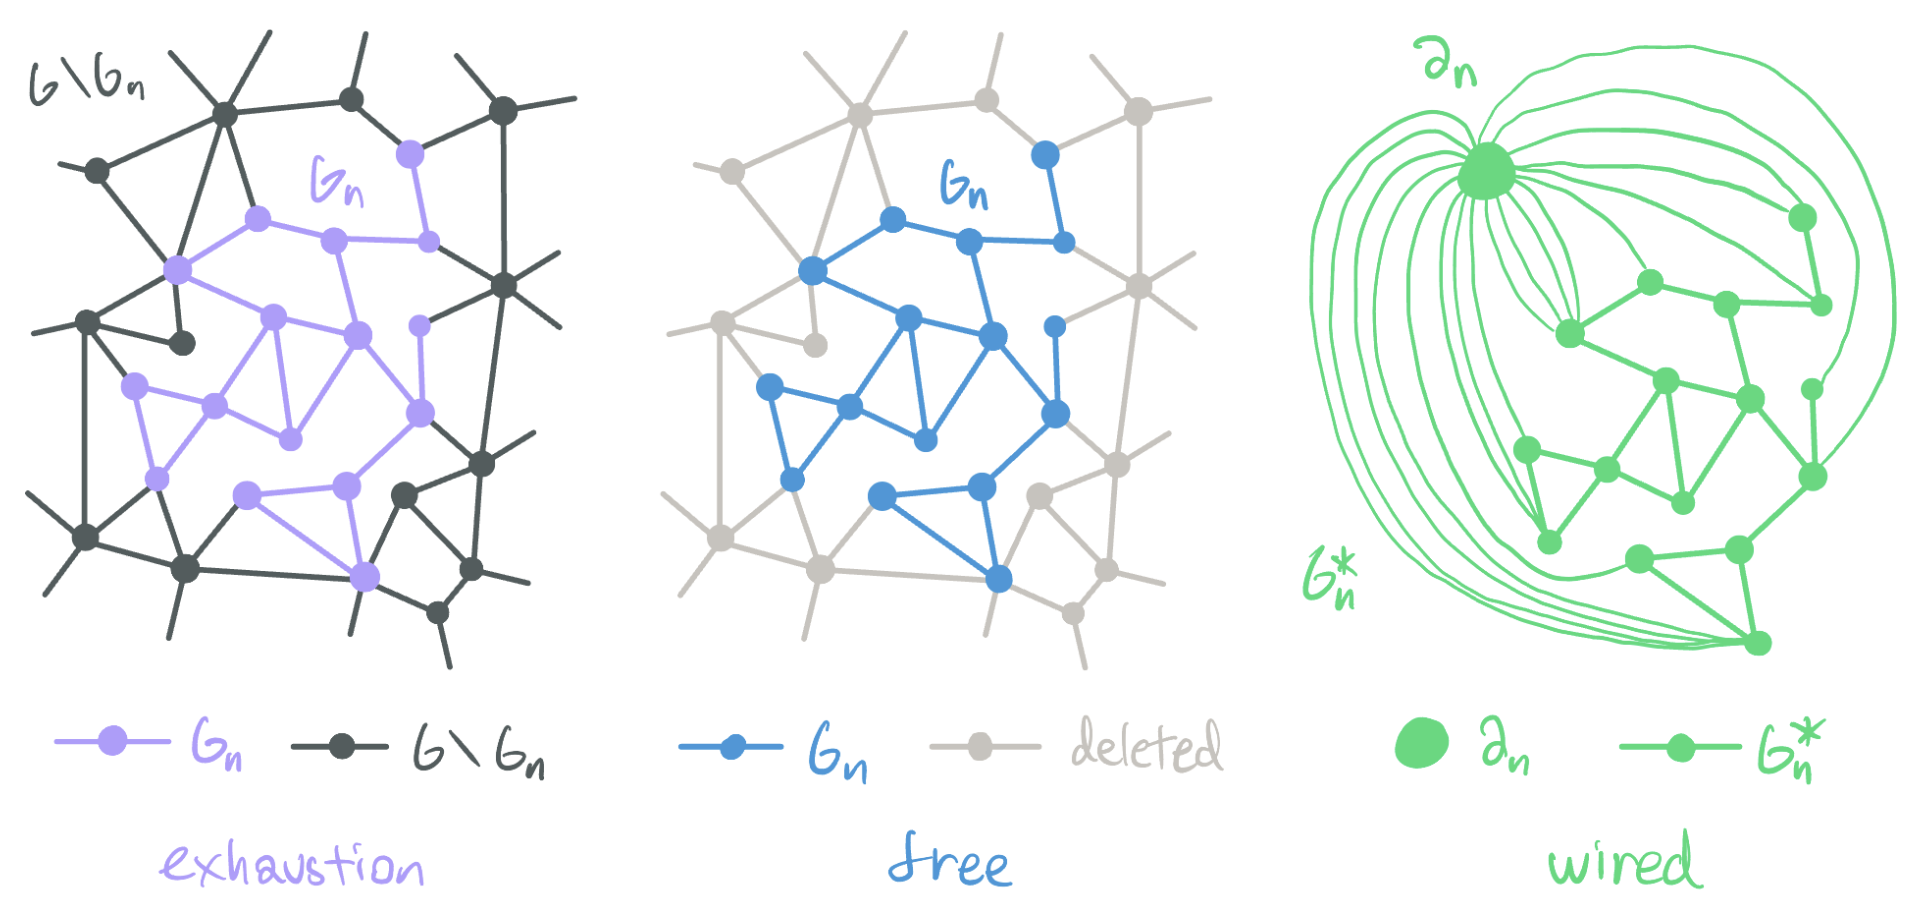
\includegraphics[width=.9\linewidth]{media/exhaustions.png}
    \caption{An illustration of the differences between the free and wired exhaustions. On the left, a subgraph (purple) is shown among a portion of an infinite graph $G$ (black). In the center, the corresponding free exhaustion $G_n$ (blue) is shown among the deleted parts of $G$ (grey). On the right, the corresponding wired exhaustion $G_n^*$ and its wired supernode $\partial_n$ are shown (green).}
    \label{fig:exhaustions}
\end{figure}

\paragraph{Free and wired exhaustions} At a particular step in the exhaustion, when we have vertex set $V_n\subseteq V$, there are two ways we can handle the rest of the graph that is not included in the subgraph $G_n$ induced by $V_n$. The first method is known as the free exhaustion, where all of $G\setminus G_n$ is deleted. The second is known as the wired exhaustion, because all of $G\setminus G_n$ is ``wired" together with the resulting self loops deleted, into a single supernode $\partial_n$. The key difference is that free exhaustions essentially destroy the boundary, because of the deletion of everything outside $G_n$, while wired exhaustions preserve the boundary edges in the form of connections to $\partial_n$ \cite{Benjamini_Lyons_Peres_Schramm_2001}.

\paragraph{Why does this matter?} Note that our study in \cref{ch:atrds} is essentially a rather degenerate case of this idea, as we only had a single node, and thus our subgraph was essentially just the single node. However, we incorporated the boundary information by way of including all incoming and outgoing flights. In this sense, the wired version was far more representative than the free version, because otherwise we would have just had nothing going on at our single node. Although most cases will not be as extreme, and even though there are reasons for going with the free method, such as simplifying the model, boundary behavior is an important consideration that we must make if we are going to be distorting our network to primarily focus on certain areas.

\section{Summary}

In this chapter, we first introduced some relevant background to help us define failures and quantify their potential severity in the stochastic setting. We covered risk preferences, then a basic formulation of risk measures, and their associated properties. Then, we covered closed-form and empirical versions of two commonly used quantile-based risk measures, VaR and TVaR, and used them to motivate the idea of distortion functions. We then covered distortion functions as a way to define spectral risk measures to generalize some of the ideas we had previously introduced. After all this, we moved on to multivariate extensions, and discussed different ways of dealing with the spatial and temporal axes. We also discussed a pattern of combining aggregation and distortion in the context of dimensionality reduction of high dimensional risk measure values. Finally, we drew some connections between those ideas and electrical networks, to motivate potential areas for future work.
\chapter{Geometry and Shrinkage}
\label{app:shrinkage}

Sometimes, it may be advantageous to incorporate ``indirect evidence'', that is, data that does not seem to be directly related to the question at hand, in order to achieve a better estimate. As a classic unintuitive example, let us briefly discuss James-Stein estimation. Suppose that over the course of the part of a season, we have gathered data on the batting averages of baseball players, and would like to predict their performance in the rest of the season. At first glance, it would seem that from the data alone, our best shot is to estimate each player's average independently, since the players themselves should perform independently of each other. However, the statistical world in 1955 received a shocking result from Charles Stein: he proved that by ``shrinking'' each individual average toward the grand mean, it is possible to obtain a lower total squared error in higher dimensional scenarios \cite{Stein_1956}. Although our focus is not quite the same thing as this particular estimation problem, we will see that the idea of shrinkage is a rather natural way to view what we were trying to do in \cref{ch:atrds}, especially once we consider a more geometric interpretation of points along a statistical manifold.

\section{Geometric Interpretation}

Back in \cref{ch:atrds}, at one step, we separately learned many different posterior distributions for each day in our dataset, and essentially combined all of this information together by learning a mapping from a label generated from contextual information and observed outcome, to a common representative posterior for a particular group of labels. This can naturally be broken up into two steps: first, clustering our many candidate distributions into meaningful groups, and second, using these groupings in combination to learn something useful together. We will call these the clustering step and combination step in the rest of this chapter, though we note that they do not necessarily have to be done separately, as we did them together earlier. However, the process that we derived was rather complicated and involved. Fortunately, in this section, and the rest of the chapter, we will introduce a more interpretable formulation. We will use it as a canvas for further directions of study, although we will not be going into as much technical detail, and will instead focus on discussing ideas.

\subsection{Natural Statistical Manifold}

To simplify the problem a bit for now, we will treat all of our contextual information, including weather, under a single $y$ variable, and include all of our observation information under a single $x$ variable. Then, we can associate each point $c=(x,y)$ in our dataset, each corresponding to a day of flights, to a learned posterior distribution for $z$, which we will call $\qvd{z;c}$. In this way, we can define a statistical manifold parameterized by $c=(x,y)$, in which each point is associated with its own probability distribution \cite{Matsuzoe_2010}, as seen in \cref{fig:example-statistical-manifold}.

\begin{figure}[htb!]
    \centering
    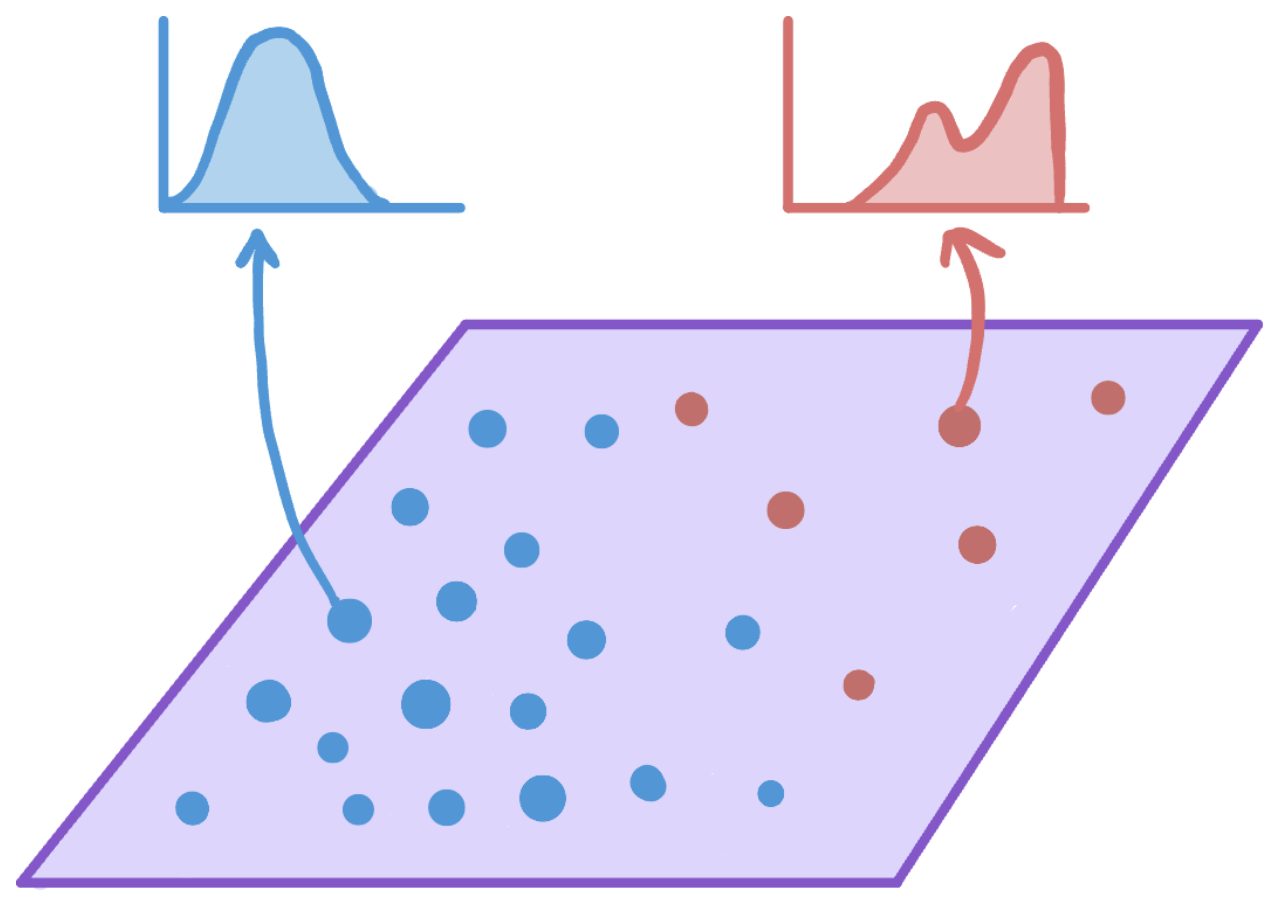
\includegraphics[width=0.5\linewidth]{media/example-statistical-manifold.png}
    \caption{An example of a statistical manifold.}
    \label{fig:example-statistical-manifold}
\end{figure}


This sort of interpretation is useful for working under an information geometric perspective. In particular, if we adopt the Fisher information metric, log-likelihood as we used earlier can be considered as a differentiable map \cite{Murray_Rice_1993}. The choice of metric is flexible, however, and depending on application, we may also want use other options such as the Wasserstein metric, which is related to optimal transport \cite{bigot2019statisticaldataanalysiswasserstein}. Note that we do not actually have access to the entire manifold. Instead, we just have observations corresponding to points on it, along with an approximated learned distribution, and we make the assumption that the latent underlying manifold is smooth. It is also useful for visualization purposes, as it can be easier to think about what we are doing with points on an object when thinking about the clustering and combination steps, than trying to directly reason with the actual mathematical objects. 

\section{Self-regularization as Shrinkage}

In this section, we will assume that we have the clustering step already taken care of, so that our data is already neatly separated into groups that we now want to work with. We have already seen a sort of self-regularization in our guiding case study in \cref{ch:atrds}, but now, we will adopt and extend an existing framework to cover our previous use case and more. In particular, we will also attempt to provide a shrinkage based reinterpretation.

\subsection{Calibrated Normalizing Flows}

First, we briefly recap the problem formulation and method as presented in the \CALNF{} work in \cite{dawson2025rare}. Rare event modeling is formulated as a data-constrained Bayesian inverse problem, where the goal is to infer the posterior distribution of latent variables $z$ from observations $\rx\sim \pld{x\given z;y}$, where $y$ are known context variables. 

\begin{example}[\CALNF{} Problem Formulation]
    We have nominal observations $\Data_0 = \{x_0^{(i)}, y_0^{(i)}\}_{i=1}^{N_0}$ and much fewer target observations $\Data_t = \{x_t^{(i)}, y_t^{(i)}\}_{i=1}^{N_t}$ available, where $N_t \ll N_0$. We wish to learn an approximation for the posterior distribution of $z$ for the target (anomaly or failure) data:
    \begin{equation}
        \qvd{z} \approx \pld{z\given \Data_t} = \pld{z\given \{x_t^{(i)}, y_t^{(i)}\}_{i=1}^{N_t}}.
    \end{equation}
\end{example}

Specifically, we use variational inference, and aim to maximize the evidence lower bound (ELBO) given by
\begin{equation}
    \elbo{}{\phi, \theta, \Data} = \EX{(x,y)\in \Data}{ \EX{z\sim \qvd{z}}{\log\pld{x,z;y}-\log\qvd{z}} }
\end{equation}
To deal with the limited target data available, \CALNF{} then adopts a bootstrapping inspired approach, where the target data $\Data_t$ is resampled into $K$ subsets $\Data_t^{(1)},\ldots,\Data_t^{(K)}$, and instead aims to learn a conditional normalizing flow $\qvd{z;c}$ where one-hot labels $c=\vone_i$ correspond to each of the target subset $\Data_t^{(i)}$, zero label $c=\vzero_K$ corresponds to the nominal data $\Data_0$, and $c^*$ is a desired optimal label representing the best mixture of the various $\qvd{z;\vone_i}$ to approximate $\qvd{z;c^*}\approx \pld{z\given \Data_t}$. 

\begin{proposition}[\CALNF{} Objective]
    The optimization problem is given by $\phi^*, c^* = \argmin_{\phi, c} L(\phi, c)$, where the loss is
    \begin{equation}
        \label{eq:calnf-loss}
        \underbrace{\beta\sum_{i\ne j} \DKL{\qvd{\cdot;\vone_i}}{\qvd{\cdot;\vone_j}}}_{\substack{\mathstrut\text{TSSO}\mathstrut\\\text{(Target Subset Similarity)}}}
        -\underbrace{\frac1K \sum_{i=1}^K \elbo{}{\phi,\theta,\Data_t^{(i)};\vone_i}}_{\substack{\mathstrut\text{TSMO}\mathstrut\\\text{(Target Subset Matching)}}}
        -\underbrace{\elbo{}{\phi,\theta,\Data_0;\vzero_K}}_{\substack{\mathstrut\text{NMO}\mathstrut\\\text{(Nominal Matching)}}}
        -\underbrace{\elbo{}{\phi,\theta,\Data_t;c}}_{\substack{\mathstrut\text{TMO}\mathstrut\\\text{(Target Matching)}}}
    \end{equation}
    where we write the mixture label $c$-specific ELBO as
    \begin{equation}
        \elbo{}{\phi, \theta, \Data; c} = \EX{(x,y)\in \Data}{ \EX{z\sim \qvd{z;c}}{\log\pld{x,z;y}-\log\qvd{z;c}} }.
    \end{equation}
\end{proposition}

\subsection{Split Likelihood Objectives}

We can see how each goal is incorporated into the overall objective $L(\phi,c)$. The last three terms in \cref{eq:calnf-loss} are the target subset matching objective (TSMO), nominal matching objective (NMO), and the target matching objective (TMO), which aim to maximize the ELBO on each target subset with labels $\vone_i$, the nominal data with label $\vzero_K$, and target data with label $c^*$, respectively. The first term is the target subset similarity objective (TSSO), which encourages similarity between the target subset posteriors, in the sense of small total pairwise KL-divergence. It is also shown that learning the mapping from labels $c$ to the candidate distributions for the posterior approximation implicitly regularizes the Wasserstein distance between the learned nominal and calibrated target posteriors.

However, although the influence of hyperparameter tuning is lessened compared to standard prior regularization methods, empirical results also showed that this learning process can be sensitive to $\beta$ in the TSSO. Specifically, empirical results showed that when the failure dataset was very small, larger values of $\beta$ which encourage similarity perform better, and when the failure dataset was larger, smaller values of $\beta$ which allow for more diversity perform better. Additionally, there are also essentially hyperparameters for the weights of the TSMO, NMO, and TMO, which are fixed at one, but this may not always be entirely appropriate.

One way we might be able to eliminate these hyperparameters entirely is by developing a principled way to specify how related the nominal data with label, target data, and target subsets, should be to each other. As we will discuss in a later section, when additional contextual information for the latent parameters is available, it can be the source of informing these similarities, though it may also be worth considering ways to do so with the current setting, such as by attempting to formalize the empirical relationship between optimal $\beta$ and relative failure and nominal dataset size.

\subsection{Generalized Calibrated Normalizing Flows}

Before we address these challenges, we will briefly consider a generalization of the \CALNF{} setup to work with multiple possibly related regimes, instead of just a simple nominal and target split. This will be relevant to our air traffic problem, as we may have many different failures modes and even different nominal modes. Therefore, consider the following generalized formulation.

\begin{example}[Generalized \CALNF{} Problem Formulation]
    We have observations $\Data_k = \{x_k^{(i)}, y_k^{(i)}\}_{i=1}^{N_k}$ for $m$ different regimes enumerated from $1$ to $k$. We wish to learn an approximation for the posterior distribution of $z$ under each regime:
    \begin{equation}
        \qvd{z} \approx \pld{z\given \Data_k} = \pld{z\given \{x_k^{(i)}, y_k^{(i)}\}_{i=1}^{N_k}}, \qquad k=1,2,\ldots,m.
    \end{equation}
\end{example}

Note that the original formulation also falls under this, as we assumed we already had sufficient data to approximate the posterior for $\Data_0$ on its own. Additionally, we could have considered each of the resampled subsets as datasets from very similar regimes, though we knew it should have been the same since they were all from the same target distribution. 

This time, we will assign labels $c_k$ to each dataset, which do not necessarily have to be the one-hot target and zero nominal encoding from before. Now, we can build the loss again, step-by-step. First, we have a direct analogue for all of the matching objectives, TSMO, NMO, and TMO, as simply the mixture label $c_k$-specific ELBO for each dataset, with an appropriate weight applied. Tackling the similarity objective, TSSO, is a bit more complicated, because may no longer be appropriate to place equal weight on the similarity for all pairs. For now, we will leave these as hyperparameters, and show how we might select them in a way that makes sense.

\begin{proposition}[Generalized \CALNF{} Objective]
    The optimization problem is given by $\phi^*, c^* = \argmin_{\phi, c} L(\phi, c)$, where the loss is
    \begin{equation}
        \label{eq:gen-calnf-loss}
        L(\phi, c) =
        \underbrace{\sum_{i\ne j} s_{i,j}\cdot \DKL{\qvd{\cdot;i}}{\qvd{\cdot;c_j}}}_{\substack{\mathstrut\text{RSO}\mathstrut\\\text{(Regime Similarity)}}}
        -\underbrace{\sum_{k=1}^m m_k\cdot \elbo{}{\phi,\theta;c_k}}_{\substack{\mathstrut\text{RMO}\mathstrut\\\text{(Regime Matching)}}}
    \end{equation}
    and we write the regime $k$-specific ELBO as
    \begin{equation}
        \elbo{}{\phi, \theta; k} = \EX{(x,y)\in \Data_k}{ \EX{z\sim \qvd{z;c_k}}{\log\pld{x,z;y}-\log\qvd{z;c_k}} }.
    \end{equation}
    Here, $s_{i,j}$ and $m_k$ are weights applied to each term in their respective objective.
\end{proposition}

Of course, one simple way to choose weights, as before, is to set all $m_k=1$ and all $s_{i,j}=\beta$. For an appropriate choice of $\beta$, or a very small value, this won't even necessarily perform abysmally, because the Regime Matching Objective (RMO) can do much of the heavy lifting if needed and if we aren't totally lacking in data for all sets. When we are lacking data, we can also still use the bootstrapping-inspired approach from the original formulation, as we can take the objectives corresponding to a target subset and split them up like before. We do have to be careful, however, about adding too many, as we may run into computational efficiency issues from having to run calculations for so many more pairings and subsets.

\begin{example}[Generalized \CALNF{} Objective with Target Subsets]
    Without loss of generality, suppose that $1,2,\ldots, l$ are target subsets that we wish to apply the resample approach to. Then, directly adding in the relevant objectives yields
    \begin{align}
        \label{eq:gen-calnf-loss-one-target}
        &\phantom{+}
        \underbrace{\sum_{i\ne j} s_{i,j}\cdot \DKL{\qvd{\cdot;c_i,\vzero_K}}{\qvd{\cdot;c_j,\vzero_K}}}_{\substack{\mathstrut\text{RSO}\mathstrut\\\text{(Regime Similarity)}}}
        -\underbrace{\sum_{k=1}^m m_k\cdot \elbo{}{\phi,\theta;k,0}}_{\substack{\mathstrut\text{RMO}\mathstrut\\\text{(Regime Matching)}}} \\
        &+ \underbrace{\sum_{k=1}^l\beta_k \spars*{
        \sum_{i\ne j} \DKL{\qvd{\cdot;c_k,\vone_i}}{\qvd{\cdot;c_k,\vone_j}}}}_{\substack{\mathstrut\text{RTSSO}\mathstrut\\\text{(Regime Target Subset Similarity)}}}
        -\underbrace{\sum_{k=1}^l \spars*{\frac{m_k}K \sum_{i=1}^K \elbo{}{\phi,\theta;k,i}} }_{\substack{\mathstrut\text{RTSMO}\mathstrut\\\text{(Regime Target Subset Matching)}}}.
    \end{align}
\end{example}

Here, we extend each label by length $K$ to augment the regime label $c_k$ with a subset label $\vone_i$ or a nominal $\vzero_K$, and adjust the granular ELBO $\elbo{}{\cdot}$ definition accordingly.

\subsection{Shrinkage Perspective}

First, going back to the original \CALNF{} formulation, the idea of prior regularization using the nominal distribution can be viewed as shrinking the learned target distribution toward the learned nominal distribution, or essentially moving to a closer point on the statistical manifold. Similarly, the resampled target subsets also experience shrinking toward each other through the similarity objective. Our generalization follows a similar idea, as we are now concerned with how much we should be shrinking each point toward each other, as controlled by the $m_k$ and $s_{i,j}$ weights.

\section{Identifying Related Failures}

In the previous section, we mainly focused on the combination step, and introduced some generalizations that required setting some hyperparameters related to similarity of different pairs of failure modes, or regimes, and of their relative influence individually. 

One case is when we already have prior distributions on the latent parameters $z$ specified. In this case, we can use the similarities of these distributions to inform what our similarity pair weights $s_{i,j}$ should be. For example, if our prior belief is that we expect regimes $i$ and $j$ to be more similar, which may be expressed by similar prior distributions for both of them, we should place a higher weight on their similarity terms. Similarly, the confidence expressed by the priors can also help inform the choice of individual influence weights $m_k$. Prior distributions that are less dispersed represent greater confidence in the belief, and so it would make sense to place a higher weight on the corresponding matching term. In our guiding case study, we had already looked into specifying prior distributions, so this was something that was sort of implicitly done during the process, albeit a bit differently.

In the remainder of this shorter section, we will also briefly discuss some ideas for when we do not immediately have this information available, and may need to work with the data only. As such, we will also focus more on the clustering step at first, since figuring out how to split our data into groups that likely come from similar distributions will help in our understanding of this problem.

\subsection{Clustering Learned Posteriors}

Let us return to our initial geometric formulation for a moment, where we have learned approximate posteriors $\qvd{z;c}$ for a collection of points $c=(x,y)$ on our statistical manifold. This is, in fact, a rather convenient representation, because as long as we have some notion of distance between two points $c_1$ and $c_2$, in a way that aligns with the similarity of their associated distributions, we can directly perform existing hierarchical clustering methods \cite{Ran_Xi_Lu_Wang_Lu_2023}. Note that our framework in \cref{ch:atrds} essentially implicitly clusters the individual per-day posteriors as part of its process, so this is something we have sort of already been doing. 

Because the structure of our data may be rather complicated, especially as we move from the single airport case to full network case, capturing the similarity between distributions may also become more difficult than before. In this case, it could also be worth applying Topological Data Analysis (TDA) methods, which attempt to extract this sort of information in a more robust manner, by studying the ``shape'' of data in a rigorous sense \cite{chazal2021introductiontopologicaldataanalysis}.

\subsection{Integrating Credibility Weighting}

One final idea we will discuss is again relevant for selecting the $m_k$ weights for our generalized \CALNF{} objective. As we mentioned earlier, the original authors found that encouraging similarity performed better for small target datasets, but for larger datasets, allowing diversity was preferable. One way we can attempt to formalize this idea and apply it to our individual influence weights is by using ideas from credibility theory. Roughly speaking, we can compare the variance of the expected values of a group, which we call the Variance of Hypothetical Mean (VHM), and the expected variance over all groups, which we call the Expected Value of the Process Variance (EVPV). Using these, we assign a credibility to the data from a group, which we can consider as analogous to our $m_k$ weights that are assigned to each dataset. Credibility decreases as EVPV increases, and increases as VHM increases. We will not go into much more detail here, as the main intent was to mention the idea of assigning importance based on the makeup of their contributions to the total variance, in terms of VHM and EVPV \cite{Buhlmann_1967}.

\section{Summary}

In this chapter, we introduced a more natural geometric interpretation of our original inference problem by viewing it as working with points on a statistical manifold. We then saw how this interpretation naturally lends itself to a shrinkage view in a generalized \CALNF{} framework for posterior approximation. Finally, we briefly discussed some clustering and credibility methods, which could be useful for setting up natural groups and weights for our generalized \CALNF{} objective.

%%% Bibliography  %%%%%%%%%%%%%%%%%%%%%%%%%%%%%%%%%%%%%%%%%%%%%%%%%%%%%%%%%%%%%%%%%%%%%%%%%%%%%%%%%

\singlespacing
\printbibliography[title={References},heading=bibintoc]

% biblatex also supports chapter-by-chapter bibliography, https://tex.stackexchange.com/a/296502/119566
% see the biblatex manual, section 3.14.3


%%%% Option for natbib %%%%%%%%%%%%%

%%   use an appropriate style (.bst) and your own .bib file[s]

%\bibliographystyle{plainnat}
%\bibliography{mitthesis-sample.bib}

\end{document} 
 